%This is the third chapter of the dissertation

%The following command starts your chapter. If you want different titles used in your ToC and at the top of the page throughout the chapter, you can specify those values here. Since Columbia doesn't want extra information in the headers and footers, the "Top of Page Title" value won't actually appear.

\pagestyle{cu}
\graphicspath{{./Chapter3/images/}}

\chapter[The First Dark Matter Search with XENON1T][The First Dark Matter Search with XENON1T]{The First Dark Matter Search with XENON1T}

XENON1T is the third generation detector of the XENON Dark Matter Collaboration.  With a fiducial mass of over 1,000 kg, it is expected to be the most sensitive detector in the world to WIMPs.  This chapter will focus on the XENON1T Dark Matter Experiment and the results from its first WIMP search.  The first section will focus on the design of the detector and its subsystems while the second section will focus on background considerations and estimation for the detector.  The following section will focus on the general calibration of the detector followed by a section on the calibration of the detector to nuclear recoils.  Finally, we will discuss the results of the first dark matter search and its implications.


\section{The XENON1T Detector}
\label{sec:xe1t_detector}

In this section we will focus on the XENON1T detector and its individual subsystems that are needed for it to operate according to the working principle discussed in \secref{sec:lxe_tpc}.  For more details on the design and construction of the detector, please refer to \citeref{aprile2017xenon1t}.

\subsection{ Laboratori Nazionali del Gran Sasso}

 Laboratori Nazionali del Gran Sasso (LNGS)  is an Italian national laboratory located underneath the Gran Sasso mountain range in central Italy.  In order to shield from cosmogenic backgrounds, dark matter detectors, and detectors for low background experiments in general, are placed deep underground.  Even deep underground, very high energy muons are still not completely shielded and are a dangerous background source for dark matter searches because they can produce fast neutrons in the rock that could recoil in the detector.  The flux of these neutrons at different laboratorias has been measured in \citeref{mei2006muon} and a plot of the fluxes is shown in \figref{fig:neutron_flux}.
 
 To shield against these cosmogenic neutrons, the TPC is inside the center of a cylinder filled with water that is roughly ten meters in diameter and ten meters tall.  This will be the focus of \secref{sec:muon_veto}. 
 
\begin{figure}[t]
	\centering
	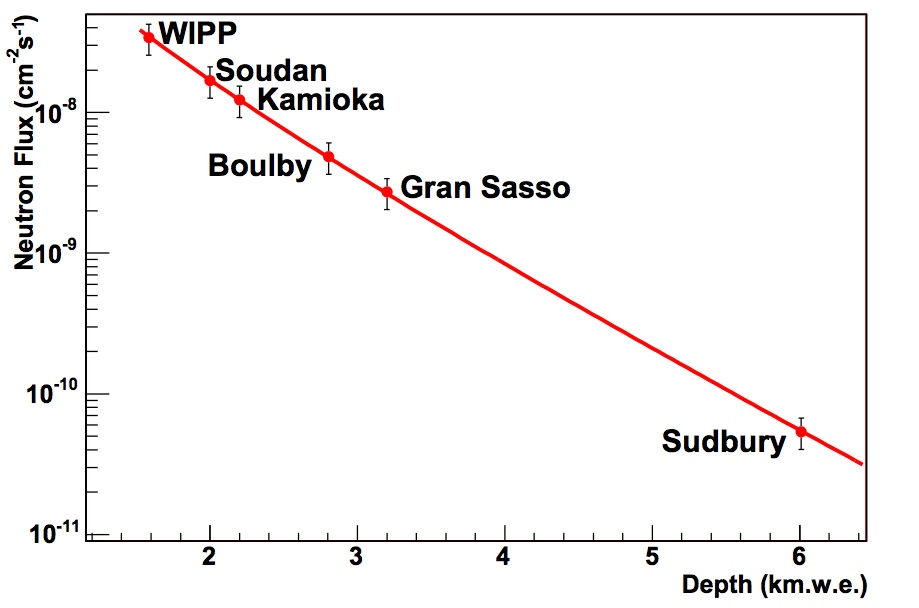
\includegraphics[width=0.8\textwidth]{neutron_flux}
	\caption{The neutron flux due to cosmogenic muons versus kilometers water equivalent depth for various underground laboratories.    Image Credit: \citeref{mei2006muon}.}
	\label{fig:neutron_flux}
\end{figure}
 
 
 \subsection{Muon Veto}
 \label{sec:muon_veto}
 
 As mentioned in the previous section, to shield against the potential cosmogenic neutron background, the TPC is placed inside of a very large water tank (~10 meter diameter and ~10 meter height).  This muon veto is outfitted with 84 8'' diameter Hamamatsu R5912ASSY high quantum efficiency PMTs to detect the light from interactions inside of the water tank and the DF2000MA reflective foil to maximize the potential measured signal \cite{aprile2014conceptual}.  A diagram showing the water tank and its PMT is shown in \figref{fig:cartoon_water_tank} and a photo of the interior of the water tank during filling is shown in \figref{fig:photo_water_tank}.  A detailed Geant4 simulation \cite{agostinelli2003geant4} of the muon events originating in the rock surrounding the laboratory shows that the efficiency of the veto is $99.78 \pm 0.05 \%$ for neutrons accompanied by the muon and $71.4 \pm 0.5 \%$ for neutrons without the initial muon.  Neutrons are accompanied by muons roughly $\sfrac{1}{3}$ of the time \cite{aprile2014conceptual}.  
 
 
 \begin{figure}[t]
	\centering
	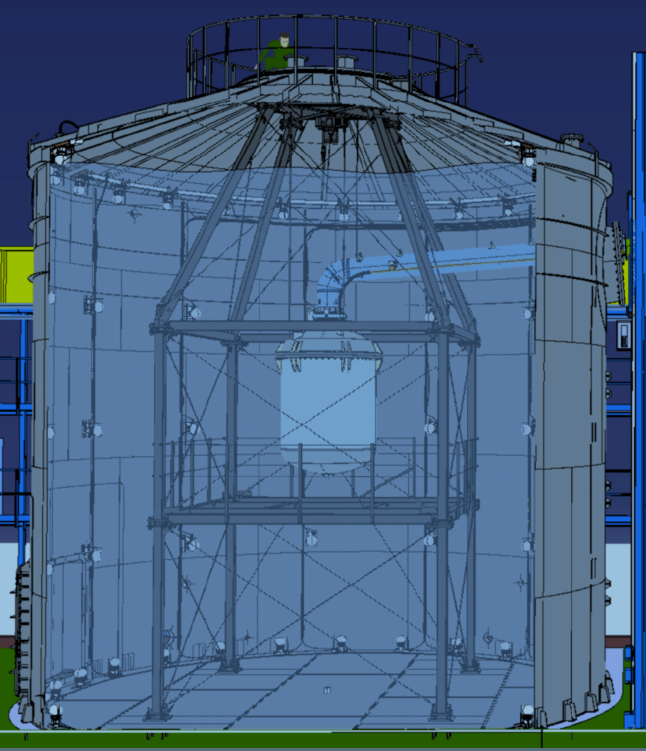
\includegraphics[width=0.6\textwidth]{cartoon_full_water_tank_muon_veto}
	\caption{A cartoon of the muon veto with the TPC centered inside the water tank.}
	\label{fig:cartoon_water_tank}
\end{figure}
 
 In addition to screening cosmogenic neutrons, the muon veto also acts as a shield to external gamma ray and neutron sources.  The neutrons mainly come from the spontaneous fission of \ce{^{238}Ur} and the \ce{^{232}Th} $(\alpha, \, n)$ reactions, both of which are found in small quantities in the surrounding rock and concrete.  Detailed Geant4 simulations \cite{agostinelli2003geant4} show that the external gamma ray background is reduced by approximately 7 orders of magnitude across 4 meters of water and the external neutron background is reduced by approximately 6 orders of magnitude per meter of water.  
 
 Given the expected fluxes for cosmogenic neutrons and radiogenic neutrons from the rock and concrete, $8.1 \cdot 10^{-10}$ above 1 MeV \cite{mei2006muon} and $8.7 \cdot 10^{-7}$ $\frac{n}{\textrm{cm}^2 \textrm{s}}$ above 1 keV, respectively, combined with the expected attenuation and cut efficiency result in a negligible external neutron background $< 0.01 \frac{\textrm{events}}{\textrm{y}}$ \cite{aprile2016physics}.
 
 
 \begin{figure}[t]
	\centering
	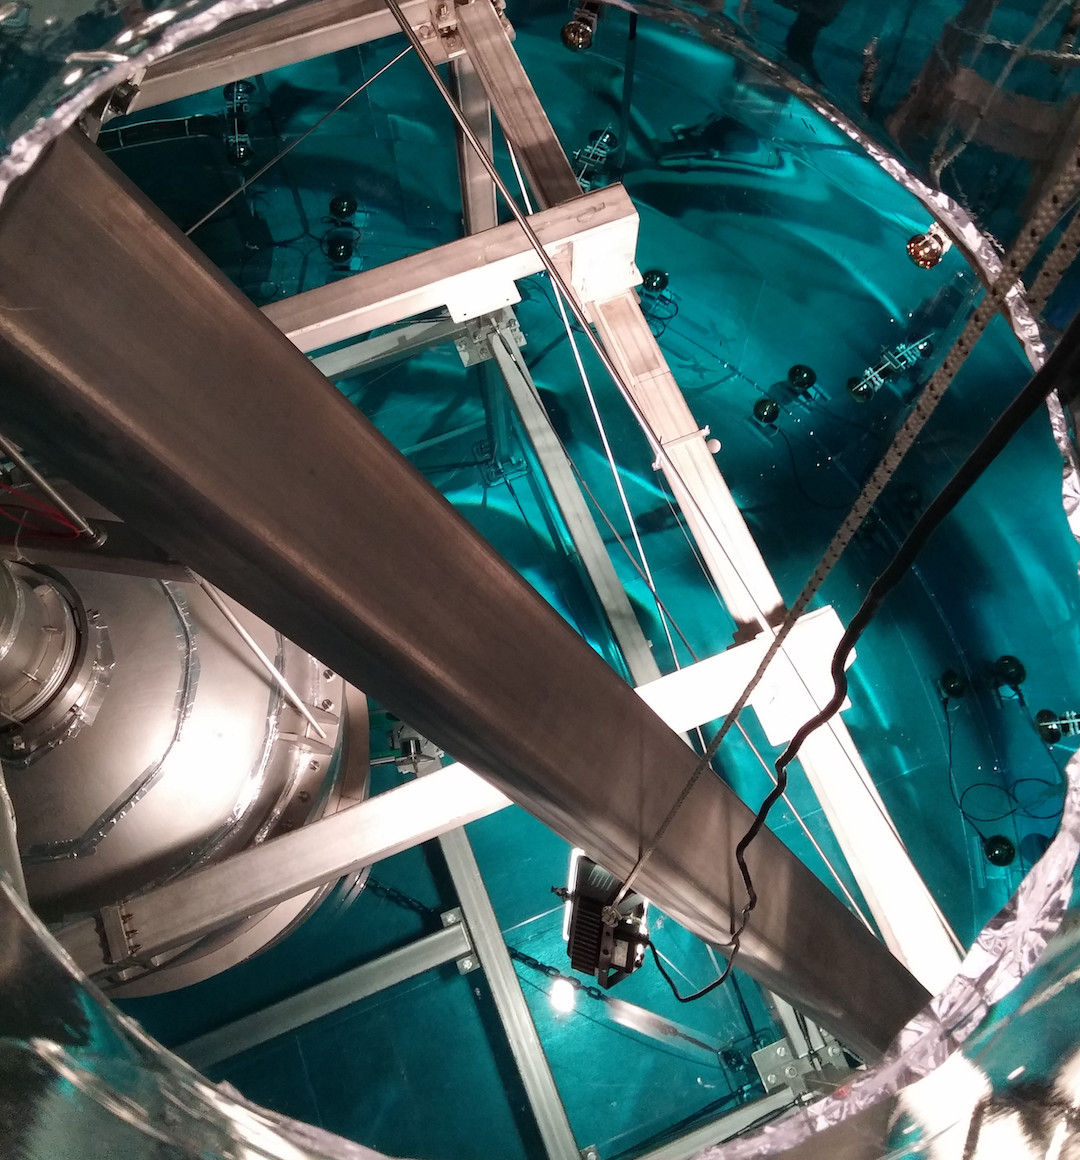
\includegraphics[width=0.6\textwidth]{water_tank_filling}
	\caption{A photo of the inside of the muon veto water tank.  The 8'' PMTs can be seen along the edges of the tank and the TPC can be seen in the center of the tank (left side of the photo).}
	\label{fig:photo_water_tank}
\end{figure}



 \subsection{Cryostat}
 \label{sec:cryostat}


In between the TPC itself and the water of the water tank is the cryostat.  The cryostat is a double-walled vacuum insulated vessel designed to contain the detector assembly and 3.5 tons of liquid xenon.  The cryostat itself is made of 5 mm thick, low radioactivity stainless steel.  The inner part of the cryostat, since it needs to house such a large amount of liquid xenon at roughly $-96^{\circ}$C, is covered in a blanket of aluminized mylar foil to minimize radiative heat transfer (shown in \figref{fig:xe1t_inner_cryostat}).  The outer cryostat is large enough to hold and support  XENON1T's inner vessel and TPC but also the inner vessel and TPC of XENONnT, a planned upgrade of XENON1T.  A diagram of the cryostat and the TPC is shown in \figref{fig:xe1t_cryostat_tpc}.

\begin{figure}[t]
	\centering
	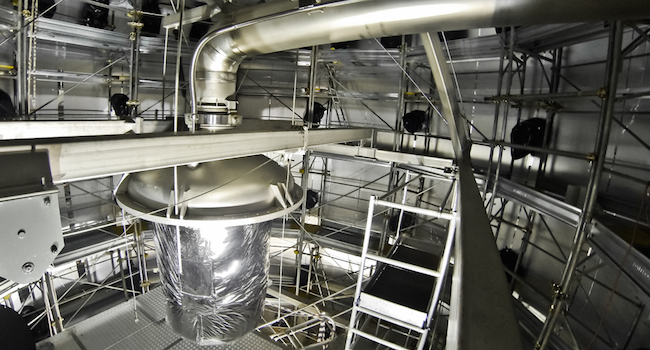
\includegraphics[width=0.99\textwidth]{xe1t_inner_cryostat}
	\caption{A photo from inside the watertank with the inner cryostat installed.  Note the mylar foil around the vessel for insulation against radiative heat transfer.}
	\label{fig:xe1t_inner_cryostat}
\end{figure}

\begin{figure}[p]
	\centering
	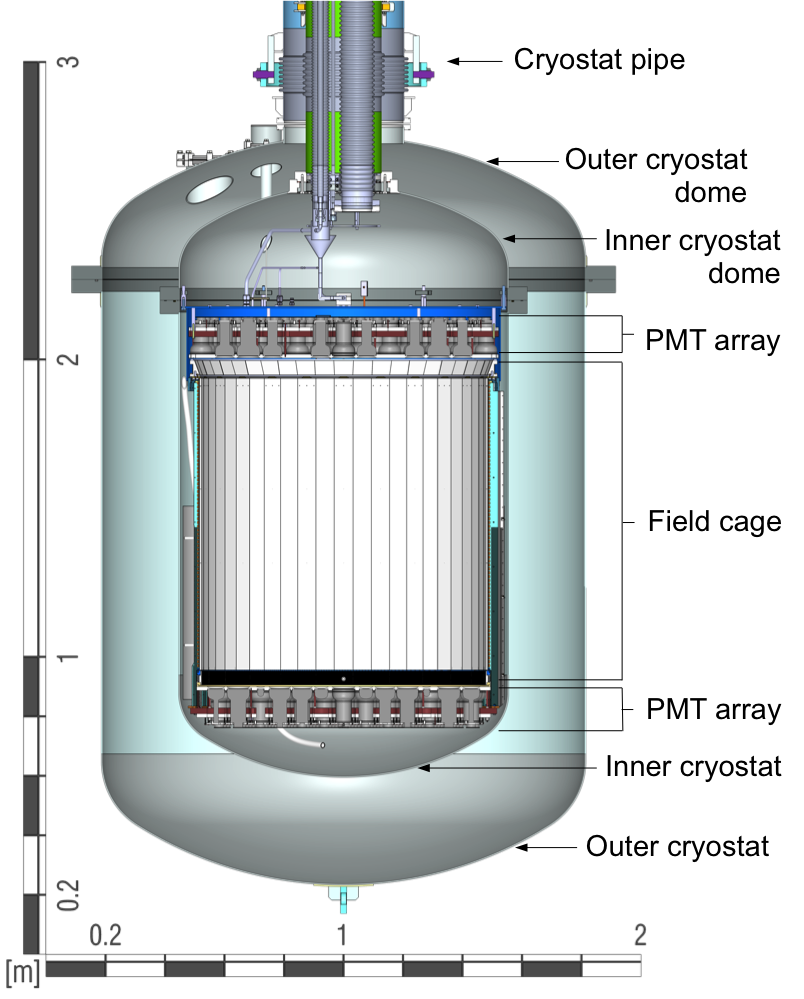
\includegraphics[width=0.99\textwidth]{xe1t_cryostat_tpc}
	\caption{A diagram of the cryostat, the TPC, and the subsystems of each.  Image Credit: \citeref{aprile2017material}.}
	\label{fig:xe1t_cryostat_tpc}
\end{figure}

The cryostat is connected to external systems such as the purification and cryogenic systems via a double-walled vacuum insulated pipe.  This pipe not only carries liquid xenon and gaseous xenon to and from the different systems but also houses the various cables that need to go into the detector (mainly signal and high voltage cables).  These cables are stored inside of a smaller pipe so that radon emanations lead away from the TPC.  One of the gaseous xenon lines is used to pressurize the xenon diving bell, which is used to set the liquid level in the detector.

The weight of the cryostat and TPC are supported by three stainless steel rods.  These rods are connected to several motion feedthroughs such that the level of the xenon in the TPC is approximately 100 $\mu$m.  These systems are also designed for XENON1T and XENONnT.

A schematic of the cryostat, TPC, and many of the subsystems that will be discussed is shown in \figref{fig:diagram_cryo_pur_sys}.


\begin{figure}[t]
	\centering
	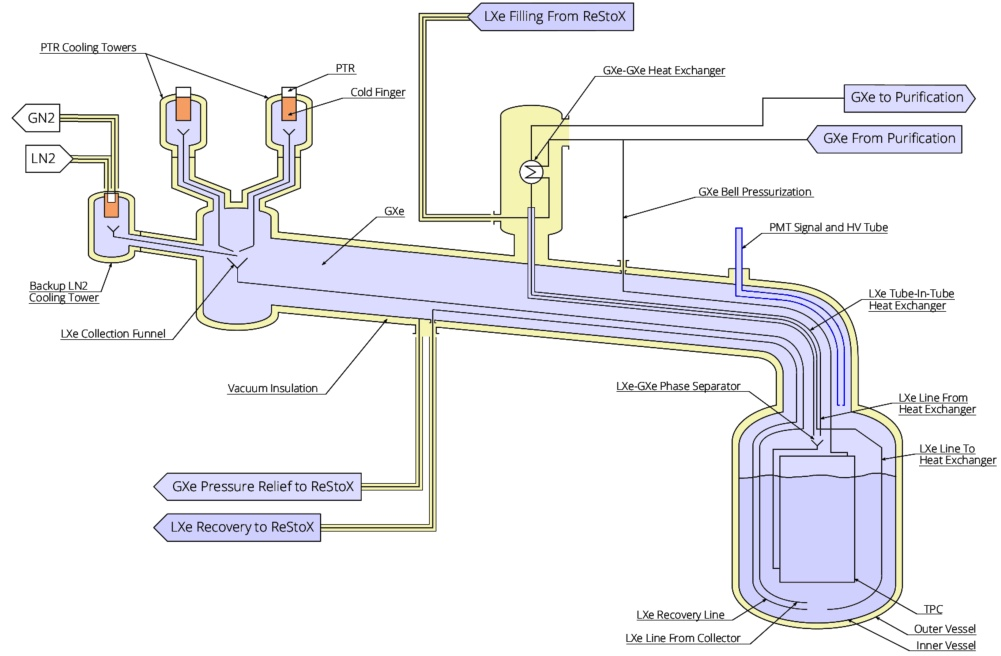
\includegraphics[width=0.99\textwidth]{diagram_cryo_pur_sys}
	\caption{A diagram of the cryostat, the cryogenics system, and the purification systems.  Image Credit: \citeref{aprile2017material}.}
	\label{fig:diagram_cryo_pur_sys}
\end{figure}


 \subsection{Cryogenics System}
 \label{sec:cryogenics_system}
 
 To keep the 3.5 tons of liquid xenon cool, two pulse tube refrigerators (Iwatani PC-150 PTRs) are used.  Each of the PTRs provides a cooling power of approximately 250 W while the estimated total heat load of the system (including the removal of electronegative impurities which will be discussed in \secref{sec:xe1t_pur_electronegative}) is less than 150 W.  Therefore, this system is doubly-redundant and designed such that a PTR can be removed and replaced during operation of the detector.  These PTRs are connected to copper cold fingers on which the gaseous xenon condensates and flows back into the detector.  The xenon pressure inside of the cryostat is controlled via resistive heaters thermally connected to the copper cold fingers.  These resistive heaters are  controlled by a proportional-integral-derivative (PID) controller that adjusts the power of the heaters to maintain a desired cold-finger temperature \cite{aprile2017xenon1t}.
 
 The photomultiplier tubes (which will be discussed in \secref{sec:photomultiplier_tubes}) are susceptible to damage if the pressure in the detector becomes too high.  For this reason, it is crucial to be able to keep the pressure stable even in the event of an emergency.  XENON1T was designed such that if there is a sudden increase in pressure, a cold finger that is cooled using liquid nitrogen is used in place of the PTRs.  To maintain normal operating conditions in the detector only ~100 liters per day are required (the tank containing liquid nitrogen can store up to 10 $\textrm{m}^3$) \cite{aprile2017xenon1t}.
 
 The three redundant cooling systems can be seen on the left side of \figref{fig:diagram_cryo_pur_sys}.  The gas in the pipe condenses on the cold fingers and then is fed back into the cryostat.

 
 \subsection{Purification Systems}
 \label{sec:xe1t_pur}
 
 There are two main purification systems in XENON1T: one for electronegative impurities and a second for the removal of \ce{^{85}Kr}.  
 
 \subsubsection{Electronegative Impurities}
 \label{sec:xe1t_pur_electronegative}
 
 As mentioned in \secref{sec:tpc_s2_sig}, electronegative impurities, mainly oxygen, enter the liquid xenon through the various materials used when constructing the detector.  These electronegative impurities can capture free electrons that are drifted to produce the secondary signal, the S2.  This causes a complete loss of signal in the case of high concentrations but will still causes large smearing effects at low levels of concentration (ppb levels of \ce{O_2} relative to xenon), reducing the discrimination power of liquid xenon for electronic and nuclear recoils.
 
Materials are cleaned before being installed in the detector however these electronegative impurities are constantly outgassing into the detector and therefore the xenon must be constantly cleaned.  To achieve high purity, a doubly redundant purification system that is connected to the cryostat is used (center of \figref{fig:diagram_cryo_pur_sys}).  This system includes two loops with a gas driving pump (CHART QDrive) and a high-termperature arare-gas purifier (SAES PS4-MT50-R getter) \cite{aprile2017xenon1t}.  The SAES getter is able to reduce the \ce{O_2}, \ce{H_2O}, \ce{CO}, \ce{CO_2}, \ce{H_2}, \ce{N_2}, and \ce{CH_4} concentrations to low ppb or below by having the impurities form irreveersible chemical bonds with the material inside of the getter.  One drawback of the getter is that it must be operated at high temperatures ($\sim 50^{\circ} \, \textrm{C}$).  However, this effect can be reduced by using heat exchangers between both the hot and cold liquid and gaseous xenon.  The gaseous heat exchanger can be seen in the center of  \figref{fig:diagram_cryo_pur_sys} and the liquid heat exchanger (tube-in-tube) can be seen on the right side of \figref{fig:diagram_cryo_pur_sys}.  These heat exchangers are approximately 96\% efficiency and significantly reduce the heat input of the getters to 0.39 $\sfrac{\textrm{W}}{\textrm{SLPM}}$ \cite{aprile2017xenon1t}.

% getter specs: http://www.saespuregas.com/Library/specifications-brochures/s110-233_a_521.pdf
 
 
 \subsubsection{\ce{^{85}Kr}}
  \label{sec:xe1t_pur_kr85}
 
 A cryogenic distillation column is used to reduce the natural krypton to xenon level to below 200 ppq (part per quadrillion).  The cryogenic distillation column leverages the different vapor pressures of the two elements around the xenon boiling point: the vapor pressure of krypton is roughly 10.8 times higher than the vapor pressure of xenon at 175 K and 2 bars.  For a dual-phase system in equilibrium, this implies that the gaseous phase will be enriched with krypton relative to the liquid by this factor of 10.8 --- this simple dual-phase system is referred to as a single distillation stage.  To improve this separation efficiency, one can put several of these distillation stages in series with each other.  This multi-stage distillation column can practically be achieved via a package material that replicates these additional stages when placed inside of a single stage.  The height of the material ultimately translates into the number of stages added \cite{fieguth2016distillation}.
 
 The concentration can be measured with an RGMS (residual gas mass spectrometer) or an RGA (residual gas analyzer).  A distillation column with 2.8 meters of the Sulzer EX package material was deployed for XENON1T and achieved natural krypton to xenon levels of $< 48$ ppq \cite{aprile2017removing}.  
 
 A similar distillation column was also built to test the possibility of radon removal.  Using 1 meter of package material, a radon reduction factor of $>$ 27 was achieved \cite{aprile2017online}.
 
 
  \subsection{Recovery and Storage}
 
 For small detectors, it sufficed to fill detectors via cooling the xenon stored in bottles and to empty the detector by evaporating the liquid xenon.  While simple, this method is inefficient and would require approximately 250 W of heating power over 2 months to fill the XENON1T detector \cite{aprile2017xenon1t}.  While an emergency situation is unlikely in XENON1T due to its many redundancies, this simple method would also make recovery of all of the xenon very difficult.
 
 Instead of storing unused xenon in bottles kept at room temperature, a new approach to recovery and storage of xenon was applied: a single 5 cubic meter vacuum-insulated stainless steel sphere rated for pressures up to 73 bar was built for this purpose, appropriately name RESToX (recovery and storage of xenon).  Similar to the detector's cryostat, several layers of aluminized mylar blanket the inner wall of this system such that the heat load on this system is only roughly 50 W.  RESToX is cooled using 16 liquid nitrogen lines that are welded to the outside of the inner wall.  To assure that the xenon inside of RESToX is kept at a precise temperature and pressure (to avoid freezing), a heating system has also been installed in the center of the vessel.
 
 RESToX is directly connected to the cryostat for filling and recuperation of the xenon gas as well as both purification systems such that the xenon stored can be kept clean and ready for use.  Xenon can be transferred into the cryostat via the pumps of the purification system (up to a maximum speed of 50 SLPM). Xenon is transferred from the cryostat to RESToX solely due to the pressure difference between the two systems.
 
 \begin{figure}[t]
	\centering
	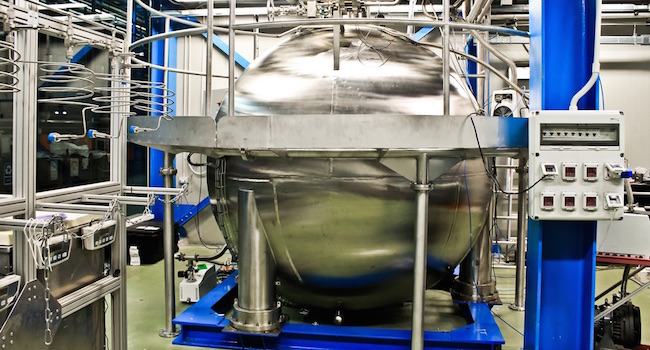
\includegraphics[width=0.99\textwidth]{xe1t_restox}
	\caption{A photograph of RESToX prior to instillation at LNGS.}
	\label{fig:xe1t_restox}
\end{figure}


  \subsection{Calibration Systems}
 \label{sec:xe1t_calibration_system}
 
While, like LUX \cite{akerib201783}, internal sources, such as \ce{^{83m}Kr}, can be injected through the purification system, a new method for introducing external sources needed to be developed due to the massive water tank surrounding the TPC.  The solution was the installation of two belts that could be used to move external sources around the bottom of the detector (the ``U-Belt'') and along the sides of the detector (the ``I-Belt'') and an additional mechanism to move the neutron generator vertically along the side of the TPC.  The main external sources used are \ce{^{228}Th} (which has several $\gamma$ lines between 511 -- 2,614 keV), \ce{^{137}Cs} (which has a single $\gamma$ line at 662 keV), and AmBe (which produces MeV energy neutrons).  The neutron generator (NSD Gradel Fusion NSD-35-DD-C-W-S) uses the deuterium-deuterium fusion process to create neutrons with energies between 2.2 and 2.7 MeV.  This generator has been specially designed to provide very low neutron rates ($\mathcal{O} \left(10 \, \sfrac{\textrm{n}}{\textrm{s}} \right)$) as well as high neutron rates ($\mathcal{O} \left(10^6 \, \sfrac{\textrm{n}}{\textrm{s}} \right)$).  These external source systems are shown in \figref{fig:xe1t_external_sources}.

Like previous generations of detectors, the PMTs are calibrated using pulsed blue light fed into the detector by fiber optic cables.  In XENON1T, four such fiber optic cables are fed into the detector at different heights and positions.


 \begin{figure}[t]
	\centering
	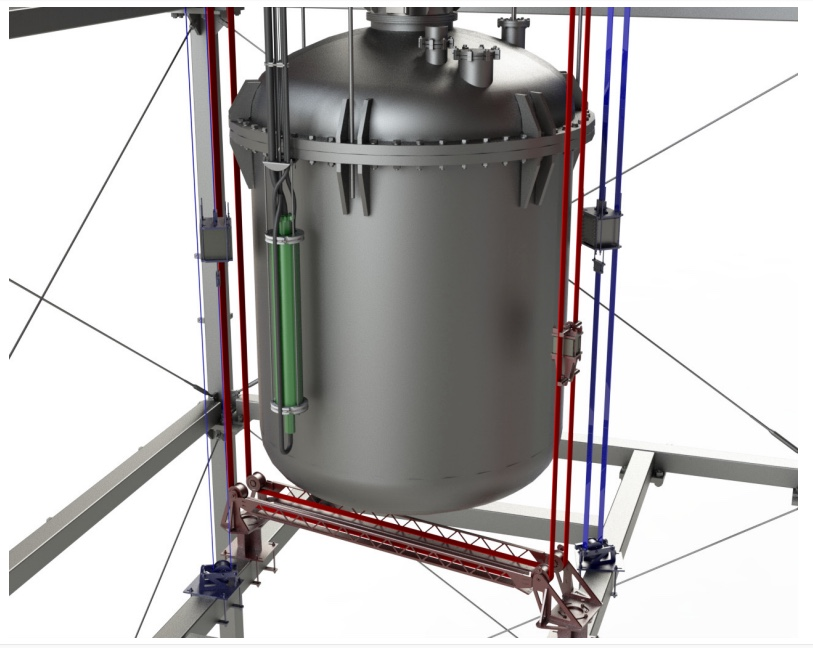
\includegraphics[width=0.7\textwidth]{xe1t_external_sources}
	\caption{A diagram showing the external calibration systems.  The ``U-Belt'', which allows for placement of external sources below the TPC, is shown in red while the ``I-Belt'', which allows for the placement of external sources at different heights along the side of the TPC, is shown in blue.  Shown in green is the neutron generator which can be raised an lowered along the side of the detector.}
	\label{fig:xe1t_external_sources}
\end{figure}
 
 
 \subsection{Photomultiplier Tubes}
 \label{sec:photomultiplier_tubes}
 
XENON1T utilizes a total of 248 high quantum efficiency  R11410-21 3 inch PMTs --- 127 of these PMTs are located in the top array and the remaining 121  are located in the bottom array.  The R11410-21 was specifically designed for XENON1T to have a high quantum efficiency, high collection efficiency, low radioactivity, and operate stably at liquid xenon temperatures.  

321 of the R11410-21 PMTs were tested for quantum efficiency, dark rate, stability, and single photoelectron response.  Of the 321 PMTs, 78 were rejected: 12 due to high or unstable dark count rate and 53 due to after-pulsing (44 of which were confirmed to have a leak).  The PMTs were found to have an average quantum efficiency of $34.5 \pm 2.8 \%$ at 178 nm and a collection efficiency of $90 - 95 \%$ \cite{barrow2017qualification}.  PMTs that were found to have a higher quantum efficiency and collection efficiency were placed in the center to maximize potential light collection as shown in \figref{fig:xe1t_pmt_qe}.  The bottom PMT array sees the majority ($\sim 90\%$) of the light for S1s due to the reflection of light at the liquid-gas interface --- therefore, the higher quantum efficiency PMTs were placed in the bottom array.

\begin{figure}[t]
	\centering
	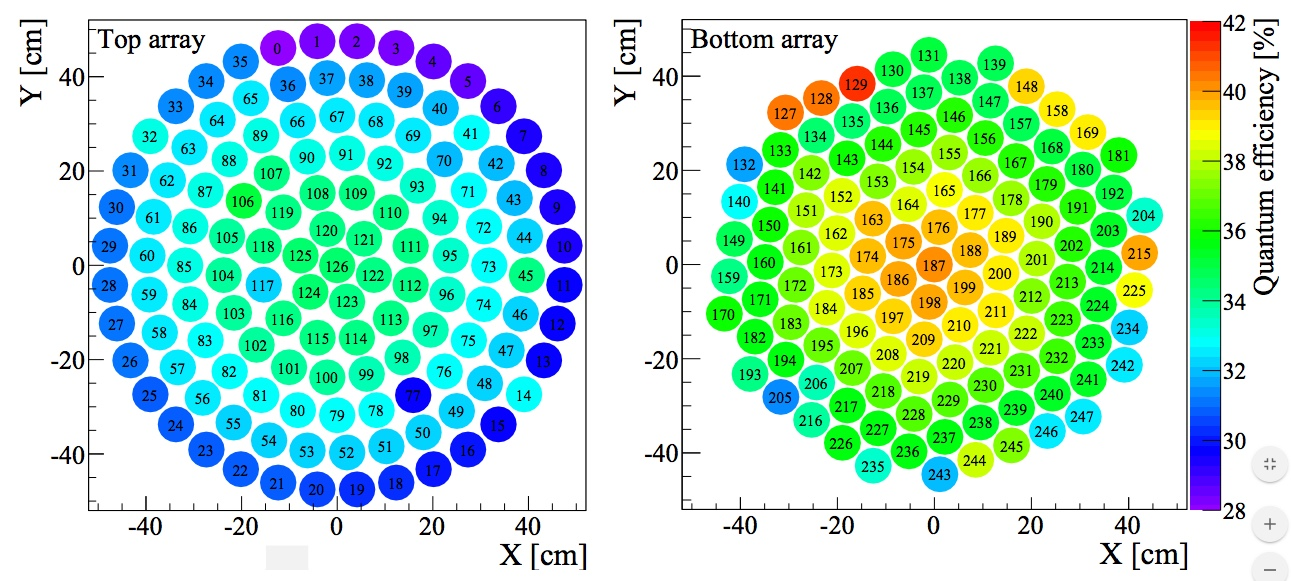
\includegraphics[width=0.99\textwidth]{xe1t_pmt_qe}
	\caption{The quantum efficiencies of the PMTs installed in the XENON1T PMT arrays.  Note that, with a few exceptions due to higher radioactivity levels, the highest quantum efficiency PMTs are placed towards the center to maximize light collection.  Also note that in general the PMTs used in the bottom array have a higher quantum efficiency than those in the top array since the much smaller S1 signal is mainly seen by the bottom array.  Image Credit: \citeref{aprile2017xenon1t}.}
	\label{fig:xe1t_pmt_qe}
\end{figure}
 
 Of the 248 PMTs installed, only 213 could be used for the first science run of XENON1T.  The reasons for omission in the final analysis varied from high levels of noise, frequent trips and flashing, and low single photoelectron acceptance at the trigger threshold.  The remaining PMTs were set such that they had a gain from $2- 5 \cdot 10^6 \, \textrm{e}^-$ and a resolution of approximately 30\%.  The gains of individual PMTs were stable over the course of data taking.
 
 % mention work on characterization of PMTs in later chapter
 
  \subsection{XENON1T TPC}
 \label{sec:xe1t_tpc}

The XENON1T has a cylindrical shape with a diameter of 96 cm and height of 97 cm at room temperature.  The TPC outer wall is made of PTFE (polytetrafluoroethylene), otherwise known as teflon.  Teflon is chosen for several reasons: it has a high reflectivity, it can be made such that it is highly radio-pure, it has low outgassing rates, it is chemically inert (so no special considerations need to be made for handling or storage), and it is an excellent insulator \cite{neves2017measurement}.  Teflon does have a high thermal coefficient of expansion resulting in a length contraction of approximately 1.4\% from room temperature to liquid xenon temperatures \cite{kirby1956thermal}.

Throughout this and second half of the previous chapter, it has been assumed that one can provide a uniform drift field in the TPC in order to extract the electrons from the interaction site to the liquid-gas interface and a uniform extraction field to extract the electrons from the liquid into the gas for amplification.  Ideally, one would use sets of parallel plates to create these uniform fields however this has the obvious drawback of not allowing for the detection of light.  Instead, the plates are replaced with ultrafine grids that can approximate a uniform field while keeping a high transparency ($\gtrapprox 90 \%$ from optical simulations).  The width of the wires used in the grids is $\mathcal{O}(0.2 \, \textrm{mm})$ and the size of the cells in the grid is $\mathcal{O}(5 \, \textrm{mm})$.  To create the two fields mentioned, the drift and extraction fields, we need three meshes: the cathode mesh ($\mathcal{O}(10-100 \, \textrm{kV})$), the gate mesh (ground), and the anode mesh ($\mathcal{O}(5 \, \textrm{kV})$).  To protect the PMTs from the high electric field, screening meshes kept at similar voltages to the PMTs ($\sim -1.5$ kV) are also installed.  To reduce edge effects and keep the field as uniform as possible out to the edge of the TPC, 74 field shaping rings made of oxygen-free high thermal conductivity copper are installed between the cathode and the anode via a chain of 5 G$\Omega$ resistors \cite{aprile2017xenon1t}.  Shown in \figref{fig:xe1t_sr0_field_sim} are the field simulations made using the final detector design and the voltages used during the first science run of XENON1T ($V_c = -12 \, \textrm{kV} \textrm{ and } V_a = 4 \, \textrm{kV}$).  

% cathode:12 kV in SR0
% anode: 4 kV
% screening: -1.55 kV (top and bottom)


\begin{figure}[t]
	\centering
	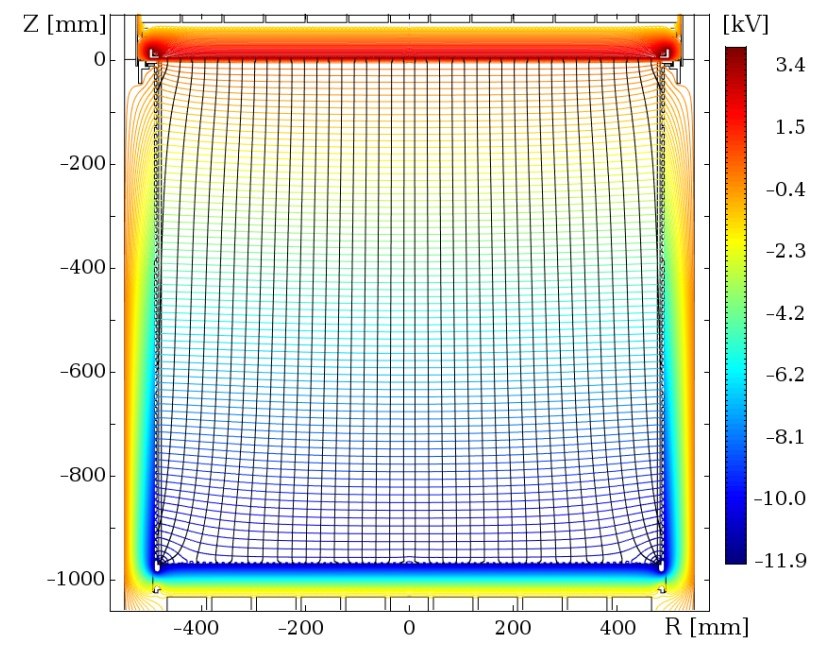
\includegraphics[width=0.99\textwidth]{xe1t_sr0_field_sim}
	\caption{The field simulations for the TPC during the first science run of XENON1T.  During this run, a cathode voltage of $-12$ kV was used and an anode voltage of $+4$ kV was used.  Image Credit: \citeref{aprile2017xenon1t}.}
	\label{fig:xe1t_sr0_field_sim}
\end{figure}


\subsection{Data Acquisition and Processing}
\label{sec:xe1t_daq_pax}

The final subsystem of XENON1T is the detector acquisition and processing system.  The signals from the 248 TPC PMTs and 84 muon veto PMTs, after being amplified by a factor of ten using a Phillips Scientific 776 Amplifier, are fed into V1724 flash ADCs.  These V1724 ADCs operate at 100 MHz (resulting in a time resolution of 10 ns), with 14 bit resolution, 40 MHz bandwidth, and a 2.25 or 0.5 V dynamic range.   Each ADC can handle eight channels simultaneously \cite{caen2017v1724}.  

The data acquisition does not have an external trigger --- instead, all pulses are digitized for each channel.  The pulses for each channel are then analyzed together to determine whether or not an event occurred and should be saved.  These events (saved as \textit{waveforms} that are just ADC counts versus time) can then be processed to extract relevant information, including, but not limited, to the size of S1 and S2 signal.  The processor, \textit{PAX} (Processor for Analyzing Xenon), was designed for XENON1T but is portable enough to be used for other dual-phase TPCs. %The efficiency of saving events using this method is found, via simulation, to be approximately 100\% after only two electrons are accelerated through the gaseous xenon given the anode voltage for the first science run.  % S1 efficiency 

Since the expected WIMP energy spectra (and most of the nuclear recoil background sources) exponentially decay with energy, it is crucially important to understand the efficiency with which events are saved and S1s and S2s are found in the events by the processor.  For the coincidence conditions, thresholds, and algorithms used in the first science run of XENON1T, it was found via simulation that S2s are identified with 100\% efficiency when produced with two or more electrons accelerated through the gaseous xenon.  This implies that even the smallest events are successfully saved.  However, given the threshold and algorithm choices of the first science run, it was found, again via simulation, that five or more photons are needed to correctly identify an S1 for an event with above an 80\% probability.  Therefore, even with the event saved, we may not be able to extract the necessary information since the processor cannot identify the S1 in the waveform.  These efficiencies will be discussed in more detail with respect to the nuclear recoil calibration of XENON1T.

\begin{figure}[t]
	\centering
	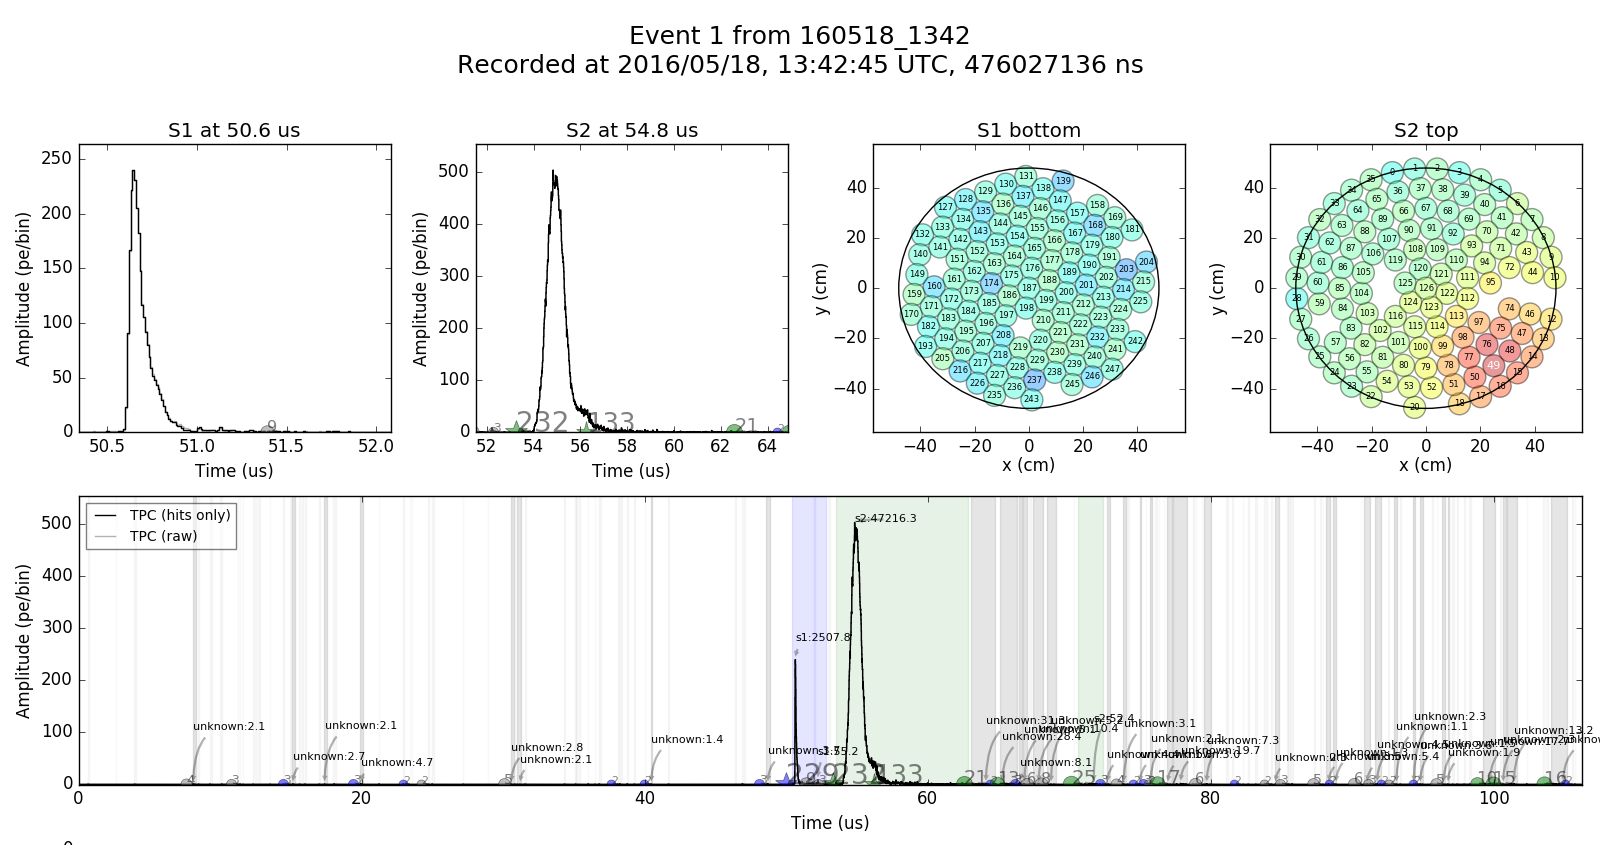
\includegraphics[width=0.99\textwidth]{xe1t_pax_output_first_waveform}
	\caption{The PAX output for the first waveform in XENON1T.  Shown in blue is the S1 and shown in green is the S2.  The grey highlighted areas represent unidentified peaks that are likely due to the high noise rate at this point in the detector operation.  Also shown are the timestamps of each signal, used to extract the depth of the interaction, and the PMT hit patterns of the top and bottom PMT arrays, which are used for position reconstruction.}
	\label{fig:xe1t_pax_output_first_waveform}
\end{figure}


\section{The Background for the XENON1T Detector}
\label{sec:xe1t_bkg}

Many of the potential sources of background were first discussed in the second chapter.  In this section we quantify the expected rate of each of these sources as a function of energy.  As mentioned previously, the higher the expected rate of background is in your region of interest, the harder it is to make a claim that excess events are due to WIMPs.  


\subsection{Background in XENON1T from Detector Materials}
\label{sec:xe1t_materials_bkg}

The first source of background that we will discuss is from the detector materials themselves.  The detector material background contributes to both the electronic and nuclear recoil background.  Even though incredible care is taken to select the most radiopure detector components for the detector, this background will prove to be non-negligible for XENON1T, as with all other dual-phase TPCs.

To quantify the background from the different detector components, materials were screened using a high-purity germanium detector and using mass spectrometry.  A detailed breakdown of the radioassay results of the various detector materials can be found in \citeref{aprile2017material}.  To estimate the background, the twelve largest background contributors and the eight most relevant backgrounds are considered \cite{aprile2016physics}.  We can simulate the background by assuming the contaminants are spread uniformly in the various detector materials and by requiring the interaction occur inside of a fiducial volume and with only a single scatter in the liquid xenon volume.  The resulting energy spectrum from the simulation for electronic recoils can be seen in \figref{fig:xe1t_er_bkg_all} and \figref{fig:xe1t_er_bkg_low} and the resulting energy spectrum from the simulation for nuclear recoils can be seen in \figref{fig:xe1t_nr_bkg}.  Each of these spectra can be integrated to determine the rate per kilogram of xenon in the fiducial volume per day.


\subsection{Electronic Recoil Background in XENON1T}
\label{sec:xe1t_er_bkg}

Even though electronic recoils can be rejected with high confidence due to their larger charge signal relative to nuclear recoils, they still pose a dangerous background for dark matter searches since the electronic recoil and nuclear recoil band overlap (as seen in \figref{fig:xe1t_disc}).  Putting aside the possibility that dark matter may interact with atomic electrons, in which case this is our most relevant background, a higher  overall rate of electronic recoils in our detectora translates to a higher probability of an electronic recoil mimicking a nuclear recoil (simply from statistical fluctuations).

The full electronic recoil background energy spectrum can be seen in \figref{fig:xe1t_er_bkg_all} and \figref{fig:xe1t_er_bkg_low}.  It is important to recall that since electronic recoils efficiently convert energy into observables, only electronic recoils under 15 keV are relevant to the WIMP search.  We will briefly discuss each component of the background in the remainder of this section with the exception of the materials background, which is discussed in \secref{sec:xe1t_materials_bkg}.

%\begin{figure}[t]
%	\centering
%	\subfloat{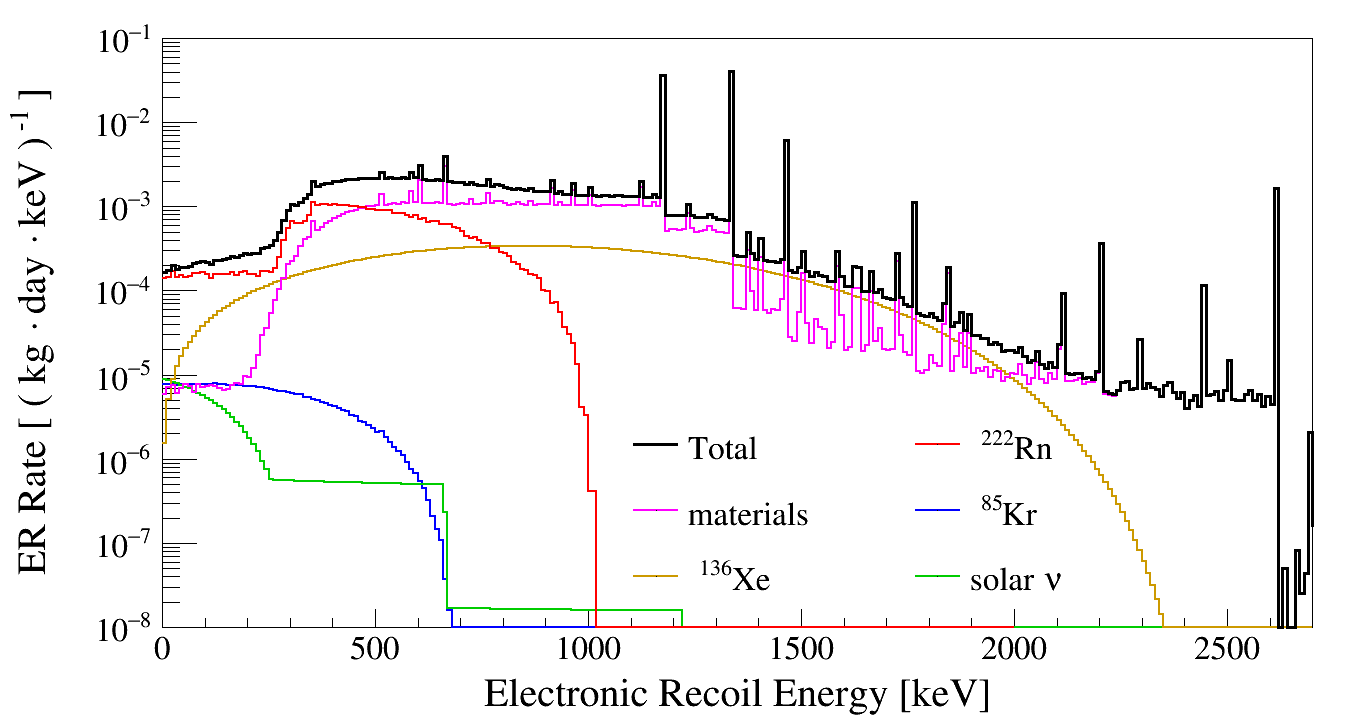
\includegraphics[width=0.5\textwidth]{xe1t_all_energy_er_bkg}} \hfill
%	\subfloat{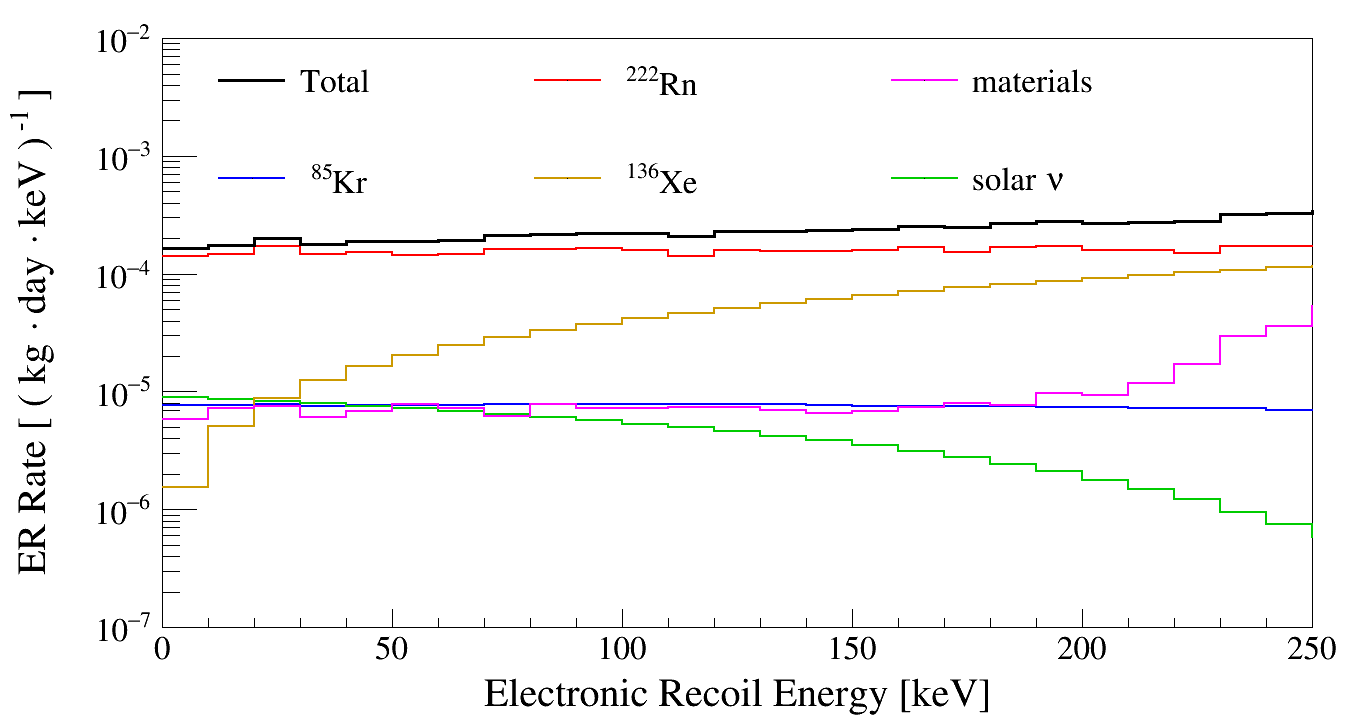
\includegraphics[width=0.5\textwidth]{xe1t_low_energy_er_bkg}}
%	\caption{.  Image Credit: \citeref{aprile2016physics}.}
%	\label{fig:xe1t_pax_output_first_waveform}
%\end{figure}


\begin{figure}[p]
	\centering
	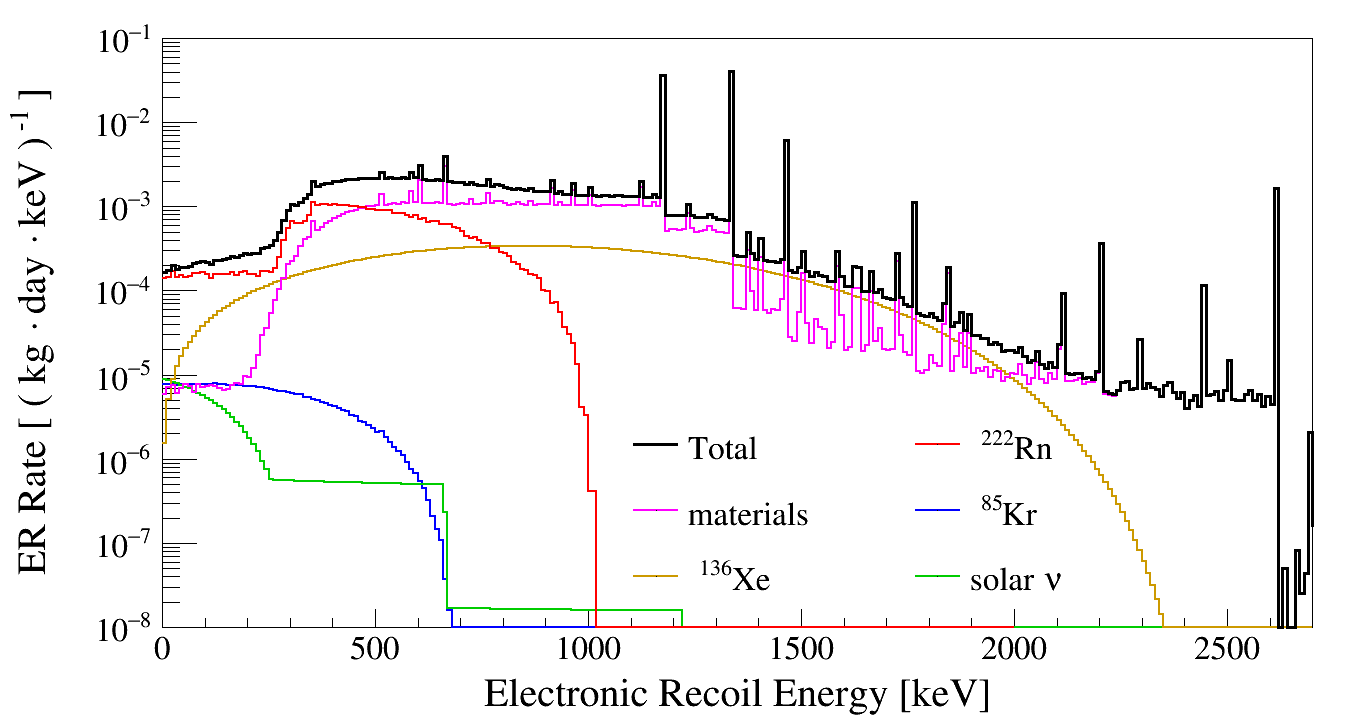
\includegraphics[width=0.95\textwidth]{xe1t_all_energy_er_bkg}
	\caption{The electronic recoil energy spectrum expected from major background sources.  While radiation from materials and the double beta decay of \ce{^{136}Xe} dominate at high energies, \ce{^{222}Rn} dominates at the lowest energies as can be seen here and in \figref{fig:xe1t_er_bkg_low}.  This low energy region is of the most concern for dark matter searches.  Image Credit: \citeref{aprile2016physics}.}
	\label{fig:xe1t_er_bkg_all}

        \vspace{\floatsep}

	\centering
	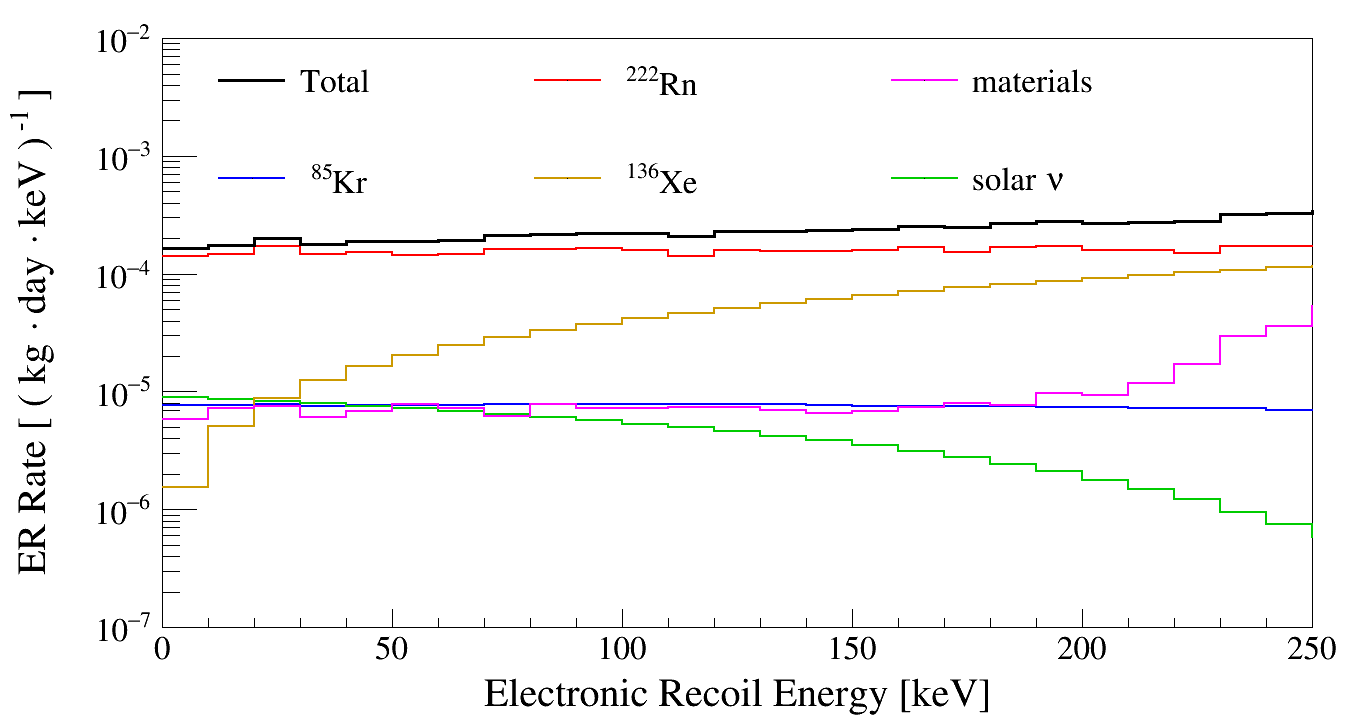
\includegraphics[width=0.95\textwidth]{xe1t_low_energy_er_bkg}
	\caption{The electronic recoil energy spectrum from background at low energies.  Note that under 15 keV, the upper threshold for electronic recoils relevant to the dark matter search, \radon{} is the dominant source of electronic recoils.  Image Credit: \citeref{aprile2016physics}.}
	\label{fig:xe1t_er_bkg_low}
\end{figure}


\subsubsection{\ce{^{222}Rn}}
\label{sec:xe1t_er_rn222}

Radon, unlike all of the other noble gasses, has no stable isotope.  Therefore, ``natural'' radon is the result of the $\alpha$ decays of \ce{^{226}Ra} into \radon{} and \ce{^{224}Ra} into \ce{^{220}Rn}.  These maternal isotopes are part of primordial \ce{^{238}U} and \ce{^{232}Th} chains, respectively, that are shown in \figref{fig:xe1t_rn_decay_chains}.  

However similar these two chains might seem, they prove to have drastically different effects for dark matter detectors.  Both \uranium{} and \thorium{}, and therefore their daughter isotopes, are found in trace quantities in almost all materials, including the ones used for the construction of XENON1T.  When either chain reaches the decay of radium into radon, the recoiling radon isotope has a chance of emanating from the surface that it is found on, for example from the inside of a stainless steel pipe into the gaseous xenon.  This is where the difference in the two chains materializes itself.  First, notice that the \uranium{} chain essentially ends at \ce{^{210}Pb} because of its long half-life.  Second, notice that with the exception of \ce{^{214}Pb} and \ce{^{212}Pb} all decays are either $\alpha$ decays or $\beta$ decays in close coincidence with an $\alpha$ decay such that events can be tagged and cut.  These two isotopes of lead both beta decay with continuous energy spectra down to zero energy, making them both potentially dangerous background.  However, the decays leading to and the decay of \ce{^{212}Pb} are relatively quick (55 seconds, 0.14 seconds, and 10.6 minutes) --- this implies that the \ce{^{212}Pb} will still be almost entirely concentrated at the edge of the detector and easily removed via a fiducial volume cut (much like the materials background).  This is clearly seen in Fig. 5 of \citeref{aprile2017results}.  On the other hand, the decays leading up to and the decay of \ce{^{214}Pb} are relatively slow (3.8 days, 3.1 minutes, and 26.8 minutes) implying that the impurity has plenty of time to spread throughout the entirety of the detector.  There is a small possibility of tagging these \ce{^{214}Pb} using the coincidence of \ce{^{214}Bi}--\ce{^{214}Po} but the 20 minute half-life of \ce{^{214}Bi} makes this very difficult.  This is why \radon{} is considered to be an intrinsic and unremovable background.

At the same time, \ce{^{220}Rn} turns out to be a very useful calibration source \cite{aprile2017results}.  Because \ce{^{212}Bi} has a half-life of approximately an hour, it has time to spread throughout the entire fiducial volume.  Additionally, the $\beta$ decay of \ce{^{212}Bi} is followed by the very fast $\alpha$ decay of \ce{^{212}Po} making these so-called \textit{BiPo} events very easy to identify.  This makes \ce{^{220}Rn} one of the most desirable electronic recoil calibration sources available with the exception perhaps of tritiated methane \cite{akerib2016tritium, aprile2017tritium}.


\begin{figure}[t]
	\centering
	\subfloat{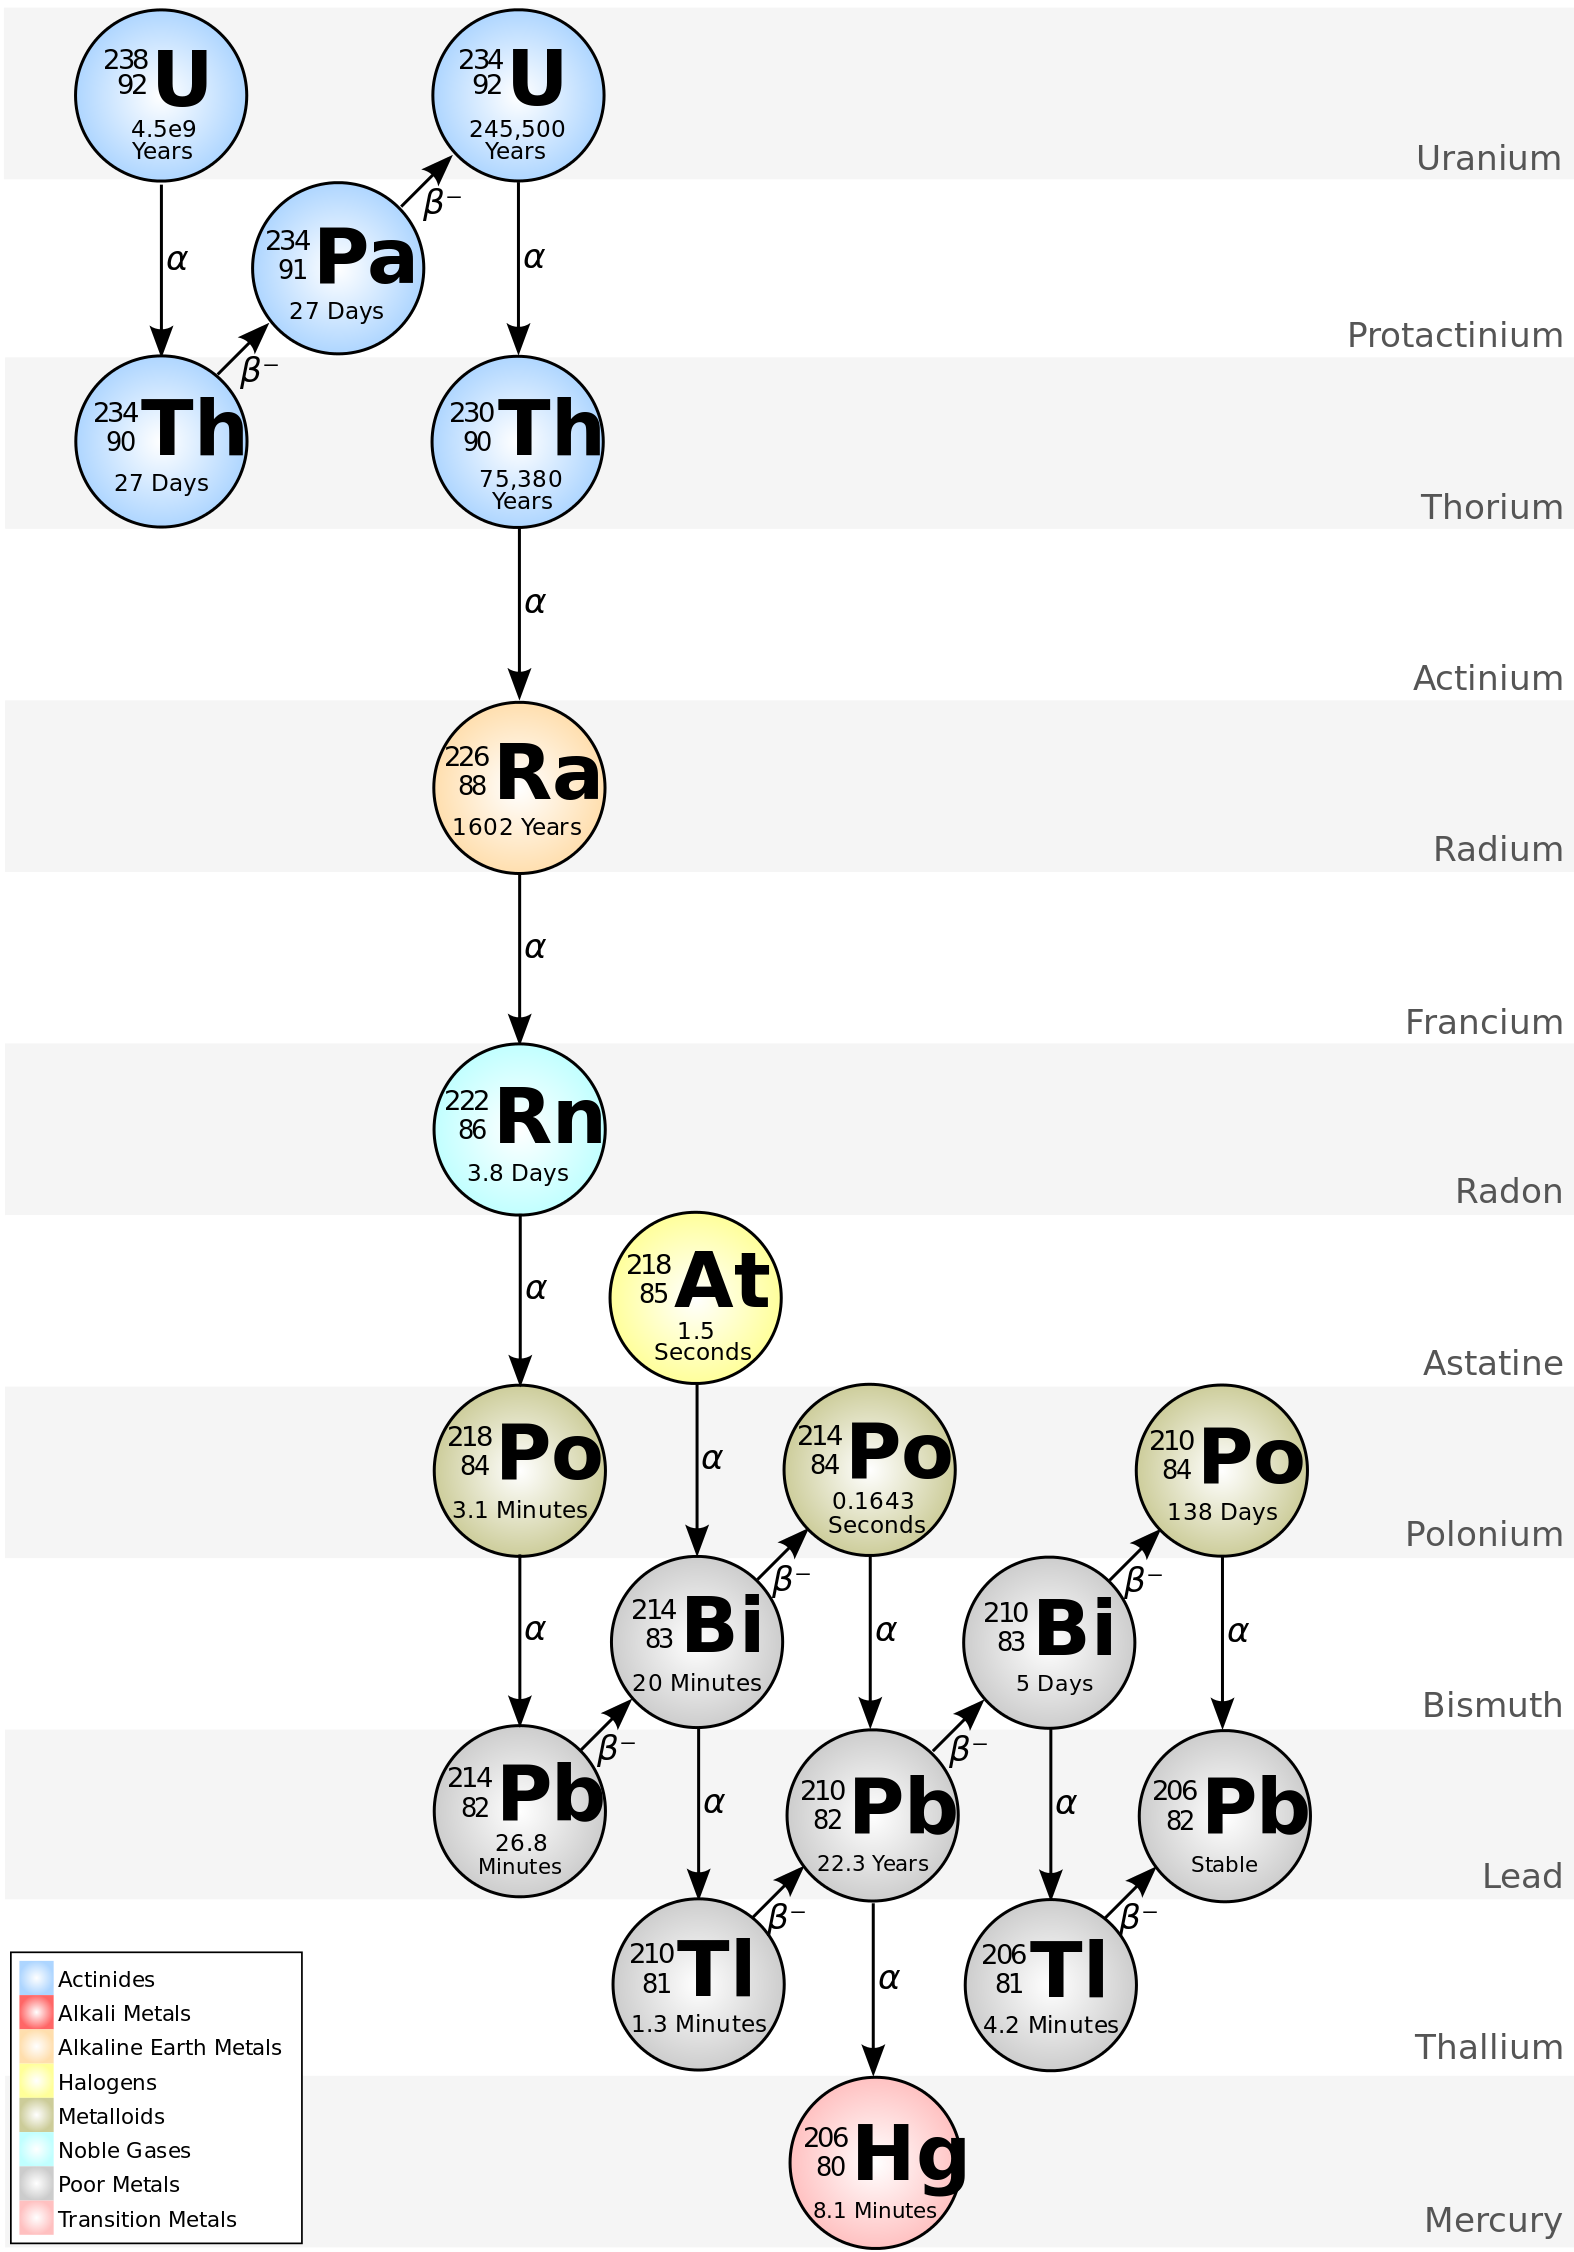
\includegraphics[width=0.5275\textwidth]{u238_chain}} \hfill
	\subfloat{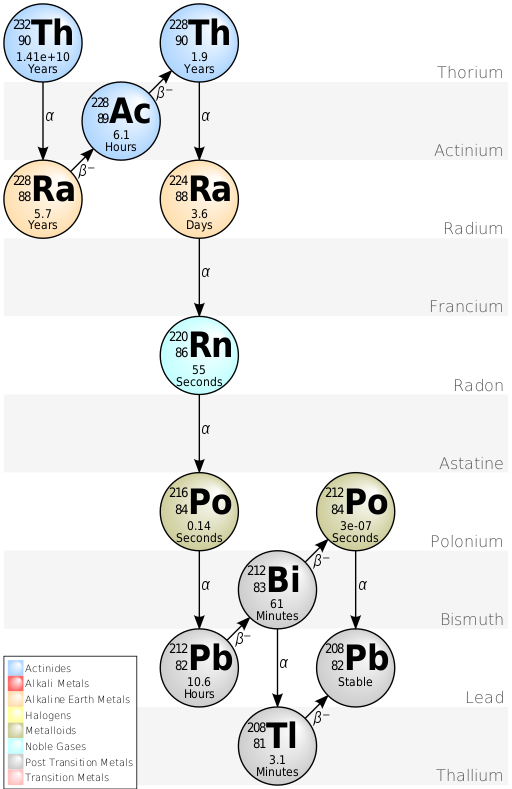
\includegraphics[width=0.4725\textwidth]{th232_chain}}
	\caption{The \uranium{} (left) and \thorium{} (right) decay chains.  The \uranium{} chain ultimately produces an intrinsic and the largest background source of electronic recoils in XENON1T while the \thorium{} chain results in a very useful electronic recoil calibration source.  Image Credit: Berkely Nuclear Forensics Group.}
	\label{fig:xe1t_rn_decay_chains}
\end{figure}


\subsubsection{\krypton{}}
\label{sec:xe1t_er_kr85}

\krypton{} is the other major internal source of background in liquid xenon based experiments.  While \krypton{} has a short half-life on a terrestrial scale (10.8 years), it is produced as the byproduct of nuclear fuel reprocessing and weapons tests.  \krypton{} $\beta$ decays with a maximum energy 687 keV with the spectrum decreasing steadily down to zero energy (as seen in \figref{fig:kr85_beta_decay}).  Commercial xenon will retain ppm to ppb levels of natural krypton (which contains \krypton{} at $2 \cdot 10^{-11}$ levels \cite{du2004atom}) as a result of the distillation process used to extract the xenon.  Due to its decay energy spectra, which allows for low energy electronic recoils, and relatively long half-life, which allows the \krypton{} due to disperse uniformly in the detector, \krypton{} is also considered to be one of the most dangerous backgrounds in XENON1T.  

Of course, ideally one would like to lower the krypton to xenon levels to as low levels as possible but the design goal of XENON1T was 0.2 ppt which translates to approximately 30 low energy electronic recoils per year in a 1 ton fiducial volume.  Using the krypton distillation column discussed in \secref{sec:xe1t_pur_kr85}, krypton to xenon levels of $0.36 \pm 0.06$ ppt were reached for the first science run putting XENON1T within a factor of two of the ultimate goal \cite{aprile2017xenon1t}.


\subsubsection{Solar Neutrinos}
\label{sec:xe1t_er_bkg_neutrinos}

Due to the mass difference between electrons and nucleons, significantly lower energy neutrinos are required for electronic recoils versus nuclear recoils.  This implies neutrinos from the sun, \textit{solar neutrinos}, will be the dominant source of neutrinos for electronic recoil background.  The energy spectra of solar neutrinos is shown in \figref{fig:solar_neutrino_flux}.  

Like electronic recoils from beta decays, the kinetic energy of the recoiling electron will follow a spectrum where only very low energies are relevant.  Unlike most of the other sources of electronic recoils, the solar neutrino background cannot be reduced and will scale with the size of the detector used.


\subsubsection{\radioxenon}

One source of background that has been mentioned in passing is the only radioisotope of natural xenon, \radioxenon{}.  \radioxenon{} was shown to decay via a \doublebeta{} decay with a half-life of $2.2 \cdot 10^{21}$ y \cite{barros2014double}.  The \doublebeta{} decay energy spectrum from \radioxenon{} is shown in \figref{fig:xe1t_er_bkg_all} and \figref{fig:xe1t_er_bkg_low} -- fortunately, unlike the beta decays resulting from the \radon{} chain and \krypton{} decay, the spectrum of \radioxenon{} decreases rapidly as electron momentum approaches zero \cite{ponkratenko2000event}.

While at the current sizes of xenon detectors this background is subdominant, it will eventually become a large source of irreducible background. 

% since radon and krypton dominated sr0 used a flat background spectrum in energy ROI

\subsection{Nuclear Recoil Background in XENON1T}
\label{sec:xe1t_nr_bkg}

Since WIMPs are expected to interact with xenon via nuclear recoils, any source of background that could cause a nuclear recoil in xenon is particularly troubling.  Care must be taken to make sure that all potenital sources of nuclear recoils are understood and accounted for --- otherwise an experiment would be susceptible to artificially strong limits or potential false discoveries.

The three major sources of nuclear recoil background are the detector materials themselves, which was discussed in \secref{sec:xe1t_materials_bkg}, neutrinos, and neutrons produced by high energy muons.  Each of these sources of background is shown in the full nuclear recoil background energy spectrum found in \figref{fig:xe1t_nr_bkg}.  

\begin{figure}[t]
	\centering
	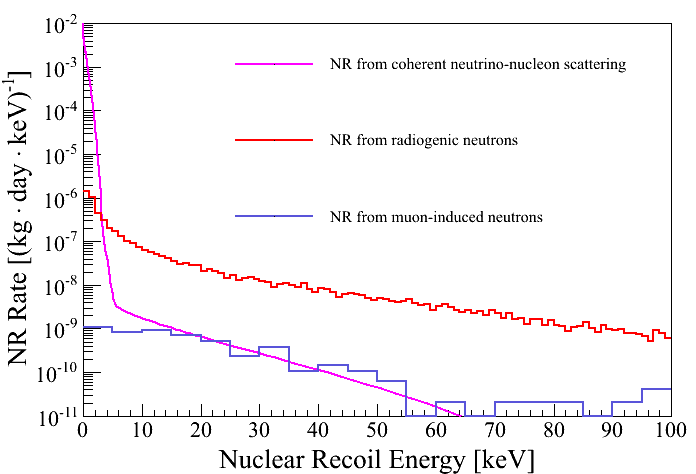
\includegraphics[width=0.95\textwidth]{xe1t_low_energy_nr_bkg}
	\caption{The energy spectra of the different sources of nuclear recoil background.  Image Credit: \citeref{aprile2016physics}.}
	\label{fig:xe1t_nr_bkg}
\end{figure}



\subsubsection{Coherent Neutrino-Nucleon Scattering}

Neutrinos can interact with both electrons, as discussed in \secref{sec:lxe_er} and \secref{sec:xe1t_er_bkg_neutrinos}, and atomic nuclei, via coherent neutrino-nucleon scattering (CNNS).  The maximum energy of a recoiling nucleus is given by $E_{\textrm{r}}^{\textrm{max}} = \frac{2 E_{\nu}^2}{m_N + 2 E_{\nu}}$, where $m_N$ is the mass of the nucleus and $E_{\nu}$ is the energy of the neutrino.  This implies that neutrinos must have energies on the order of 10 MeV to cause nuclear recoils on the order of 1 keV.  Therefore, high energy neutrino sources like \ce{^{8}B} in the sun as well as neutrinos from supernovae and the atmosphere will contribute the most to the CNNS background in dark matter experiments.

Unlike radiogenic nuclear recoils from radiogenic neutrons and muon-induced neutrons, this background cannot be shielded and cannot be reduced, in any reasonable sense, by a fiducial volume cut.  Therefore, as dark matter detectors become more and more sensitive this will constitute an irreducible background.

\subsubsection{Nuclear Recoils from muon-induced neutrons}

We discussed the possibility of a neutron background as the result of high-energy cosmogenic muons interacting in the rock and concrete surrounding the laboratory and the detector in \secref{sec:muon_veto}.  Given the efficiency of the muon veto and the low flux of muons expected because of the rock above the laboratory, the expected rate of nuclear recoils from muon-induced neutrinos is extremely low, as can be seen in \figref{fig:xe1t_nr_bkg}.



\section{The Calibration and Characterization of XENON1T for the First Science Run}
\label{sec:xe1t_calibrations}

In this section we will discuss the most important calibrations needed for the first science run of XENON1T.  We will also briefly discuss the basic cuts made during the first science run and their acceptance.  All of these cuts and calibrations are necessary for the discussions of the following two sessions regarding the calibration of XENON1T to nuclear recoils (performed by the author) and the first dark matter search.


% SPE
% position correction

\subsection{PMT Characterization}
\label{sec:xe1t_pmt}

One of the most basic tasks in TPCs of any size is to characterize the response of PMTs (\secref{sec:photomultiplier_tubes}) to photons that create a single photoelectron (SPE).  While the ideal case is that we completely understand the shape of the response function of the PMT (essentially the probability distribution function of how large the output signal will be given a single photoelectron), most experiments settle for understanding only the mean and variance of the distribution.  The reason for this practical compromise is that the single photoelectron response of a PMT is roughly normal and that when dealing with a large number of photoelectrons ($\gtrapprox 20$ PE), by the central limit theorem, the response will appear to be a normal distribution defined by only the mean and the variance of the single photoelectron response.  Therefore, an understanding of the full photoelectron response will never be necessary for S2s, even for the smallest signals.  However, a full understanding of the response of a PMT to a single photoelectron could be beneficial in understanding very small S1 signals.

Two methods were used to characterize the response of the PMTs for XENON1T during the first science run.  Both involved using low levels of blue light to illuminate the PMTs such that the probability distribution of photons detected is approximately Possonian.  The first method involves assuming a distribution for the background distribution (no light detected) and the SPE response and using these assumptions to fit the low light spectrum.  In XENON1T, it was assumed that the background distribution is Gaussian with an exponential component and that the single photoelectron response, before convolution with the background, is Gaussian.  A sample fit with the labeled components is shown in \figref{fig:xe1t_spe_gaussian}.



\begin{figure}[t]
	\centering
	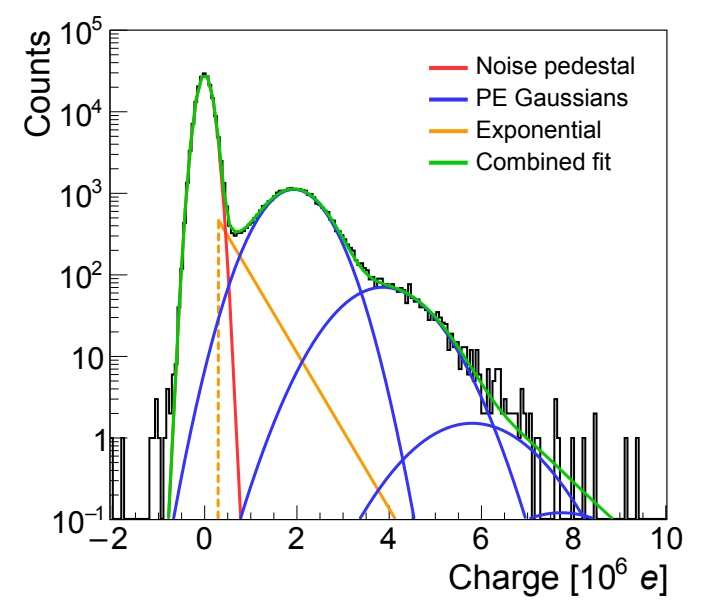
\includegraphics[width=0.8\textwidth]{xe1t_spe_gaussian}
	\caption{A fit of the low light response of one of the XENON1T PMTs in order to characterize the single photoelectron response.  Image Credit: \citeref{barrow2017qualification}.}
	\label{fig:xe1t_spe_gaussian}
\end{figure}


The second method used to calibrate the charge response of single photoelectrons in a completely statistical and model-independent way.  While this method requires a background measurement that is completely compatible with the measurement at low light levels (for example, the electronics of the light source causing additional background would be an example of incompatability), one can extract the mean and variance of the single photoelectron response very easily and without assumptions \cite{saldanha2017model}.

PMT characterization will be discussed in much further detail in the next chapter where we will describe a method that the author developed for the non-analytical characterization of PMTs using the cascade model.




\subsection{Position Reconstruction}
\label{sec:xe1t_pos_rec}

It has been mentioned several times that TPCs have the unique capability of reconstructing the three-dimensional position of an interaction within a detector.  We will now discuss how the interaction vertex was found during the first science run of XENON1T.

As was discussed in \secref{sec:xe_pos_rec}, in a dense medium such as xenon with a large uniform electric field across it, one would expect that free electrons are quickly accelerated to their drift velocity and stay at this velocity until reaching the liquid-gas interface.  Therefore, if one knows the drift velocity at the given electric field then one can measure the depth of the event from the drift time (very closely estimated by the time difference between the S1 and S2 of a given event).  Measuring the drift velocity is very simple --- the distance between the cathode and the gate (which is just below the liquid-gas interface) is known so by looking at the maximum drift time (the time it takes to travel from the cathode to the gate) one can approximate the drift velocity at the given field.  The maximum drift time can be found using a spectrum like the one shown in \figref{fig:xe1t_drift_time_vs_width}.  For the first science run of XENON1T, the maximum drift time to cover the 96.9 cm at approximately 12 \sfrac{kV}{cm} was 673 $\mu$s which gives a drift velocity of 1.43 \sfrac{mm}{$\mu$s}.


\begin{figure}[t]
	\centering
	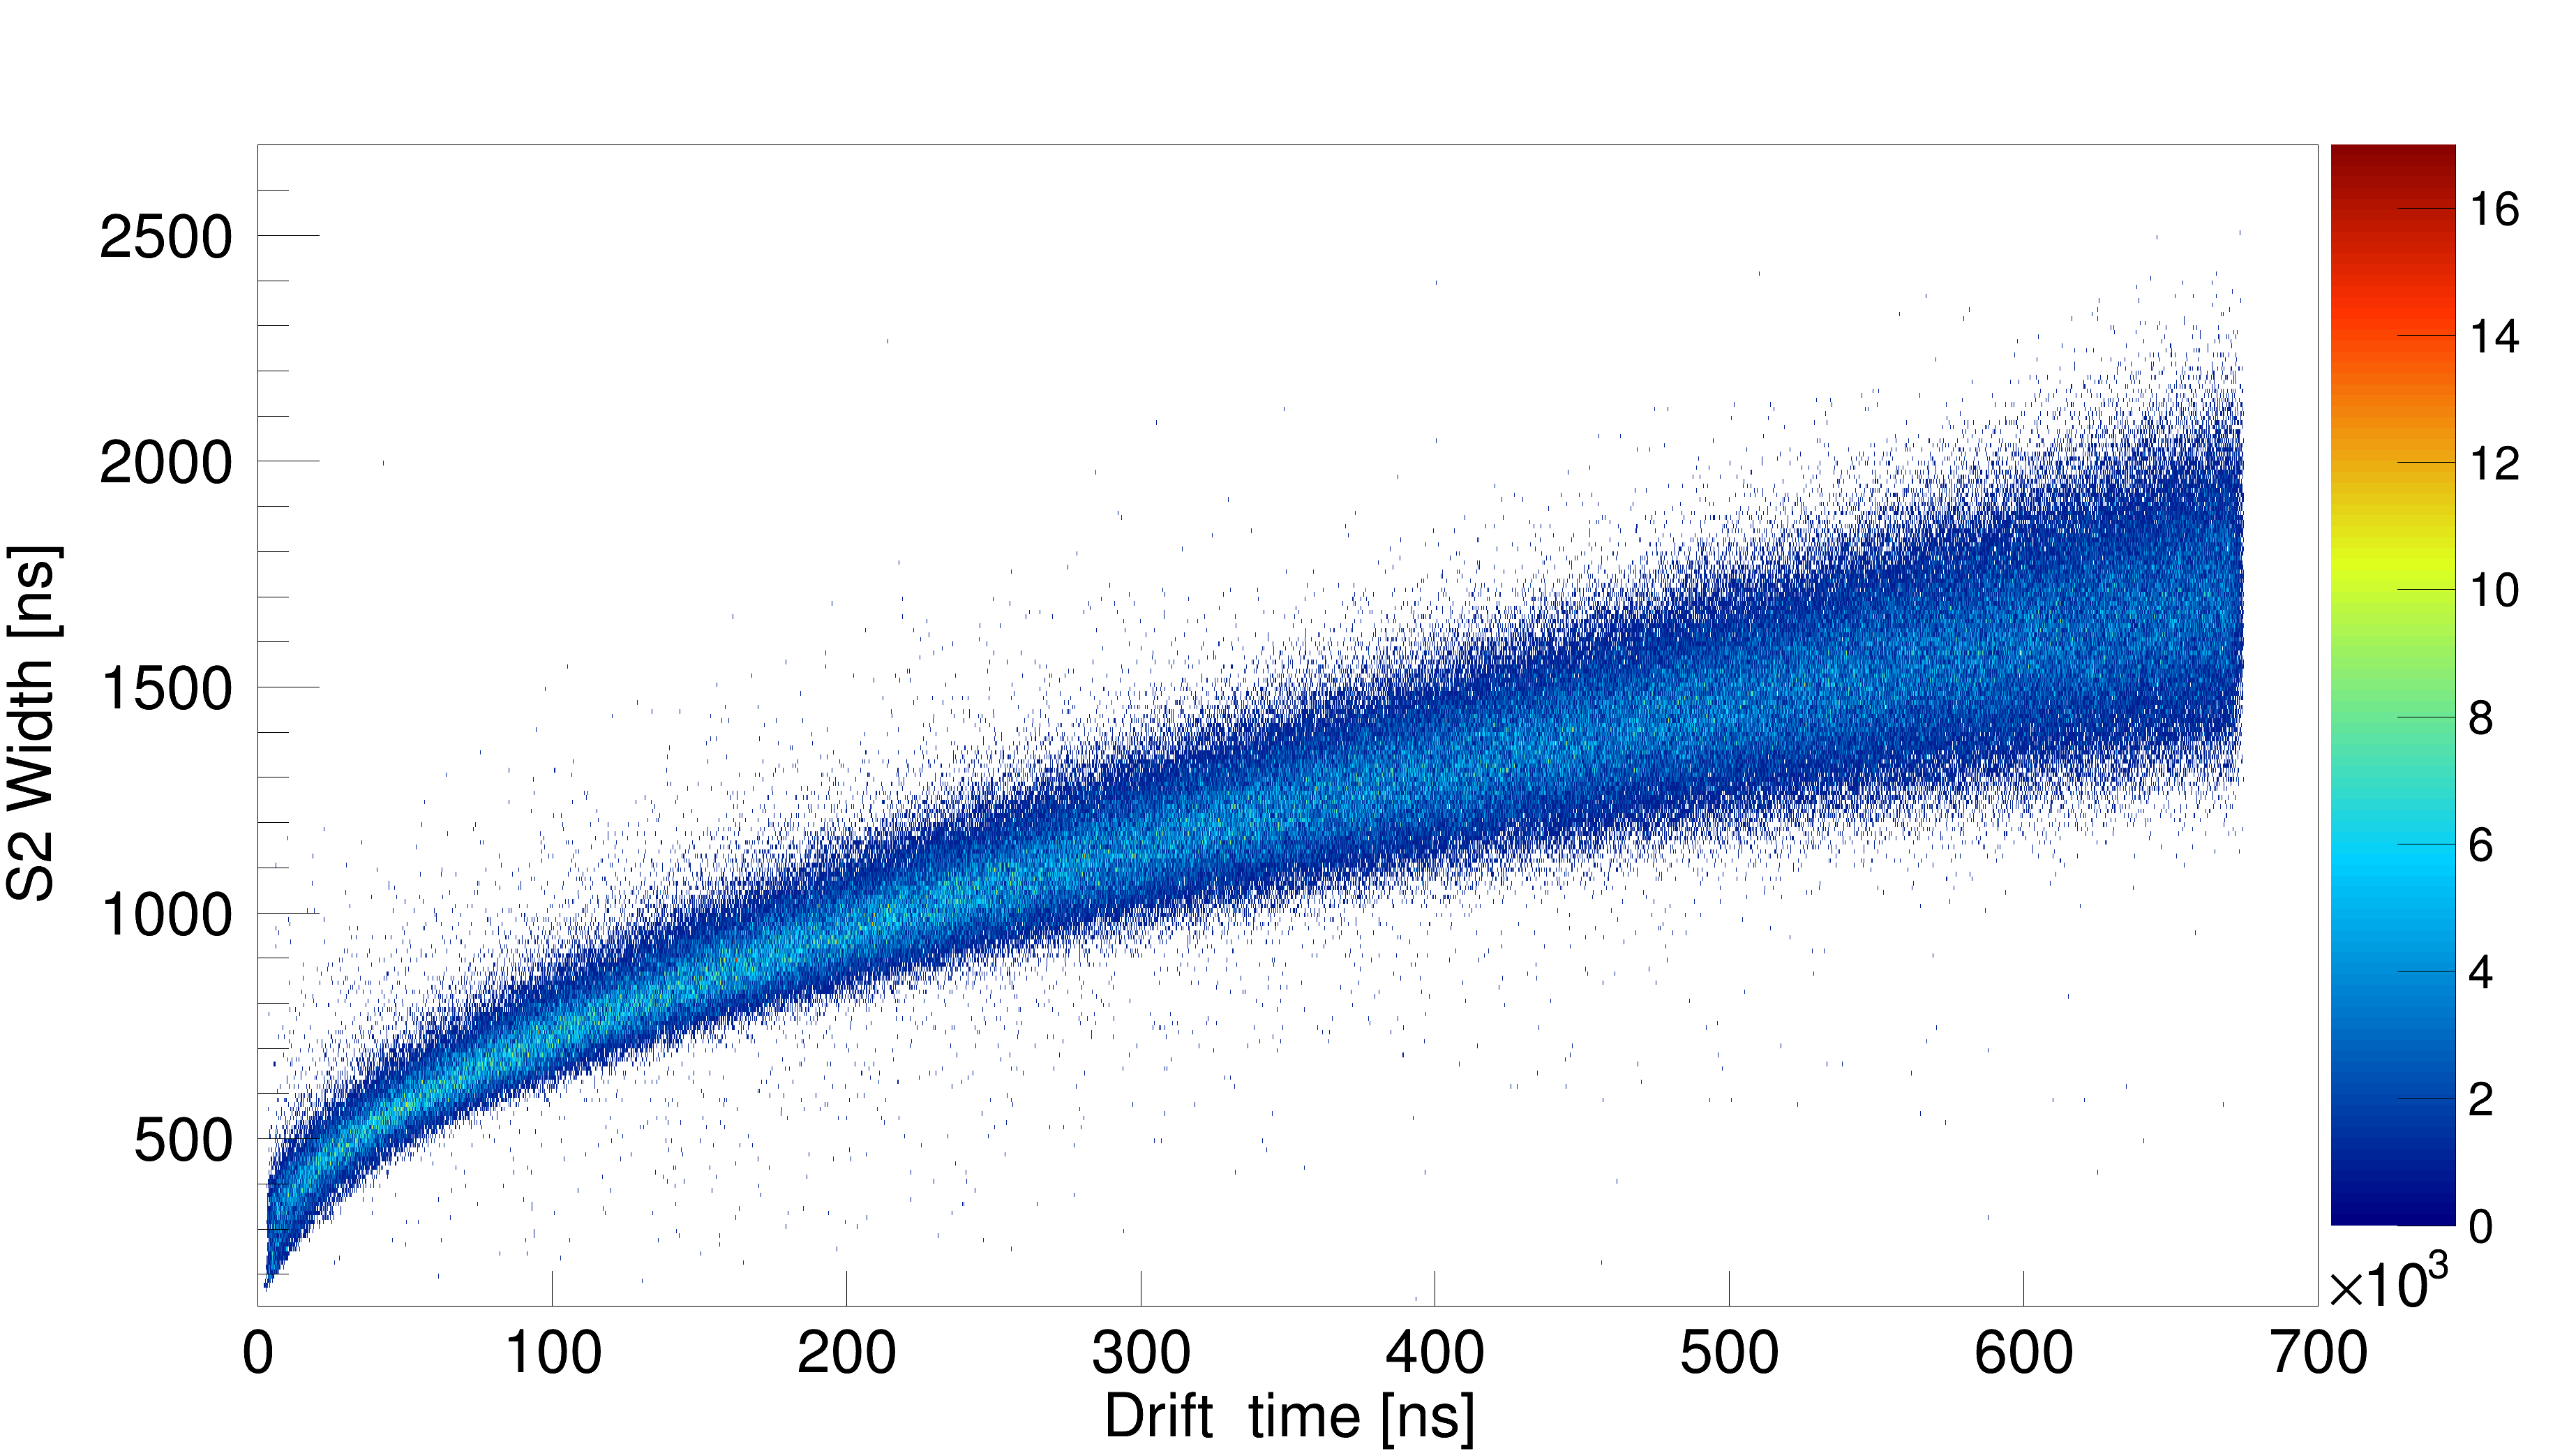
\includegraphics[width=0.99\textwidth]{xe1t_drift_time_vs_width}
	\caption{A plot of the width of an S2 versus the drift time for 32 keV events from \ce{^{83m}Kr}.  Note that at a certain drift time, no more events are seen.  This cut-off in events represents the location of the cathode since interactions below it will not produce an S2.}
	\label{fig:xe1t_drift_time_vs_width}
\end{figure}


Finding the location of electron extraction (a good proxy for the position given the field uniformity in the detector) for an event can be done by looking at the light pattern resulting from a given S2.  While this might seem relatively simple, consistently reconstructing the position within 2 cm of its actual location is a very complicated task due to detector effects.  Current methods of position reconstruction are reliant on simulation to produce either training data for a neural network or light collection efficiency maps for each of the top PMTs.  

While using multiple algorithms for position reconstruction is useful for consistency checks, ultimately only one algorithm can be used.  In the first science run of XENON1T, the algorithm used the simulated light collection efficiency maps for each PMT as part of likelihood function to find the position in the highest agreement with the measured pattern.  This method resulted in a less than 2 cm mean reconstruction error for simulated data with a signal size above the trigger threshold.  This error continuously decreases as the size of the S2 signal increases.  The more important test, though, is how the algorithm reconstructed the position of real events in the detector.  While we cannot compare positions event-by-event, we can look at the overall distribution of positions for a given source and compare that to our expectations.  \figref{fig:xe1t_pos_rec_kr} shows the distribution of positions in all dimensions for 32 keV events from \ce{^{83m}Kr}, which should be uniformly distributed inside of the detector.


\begin{figure}[t]
	\centering
	\subfloat{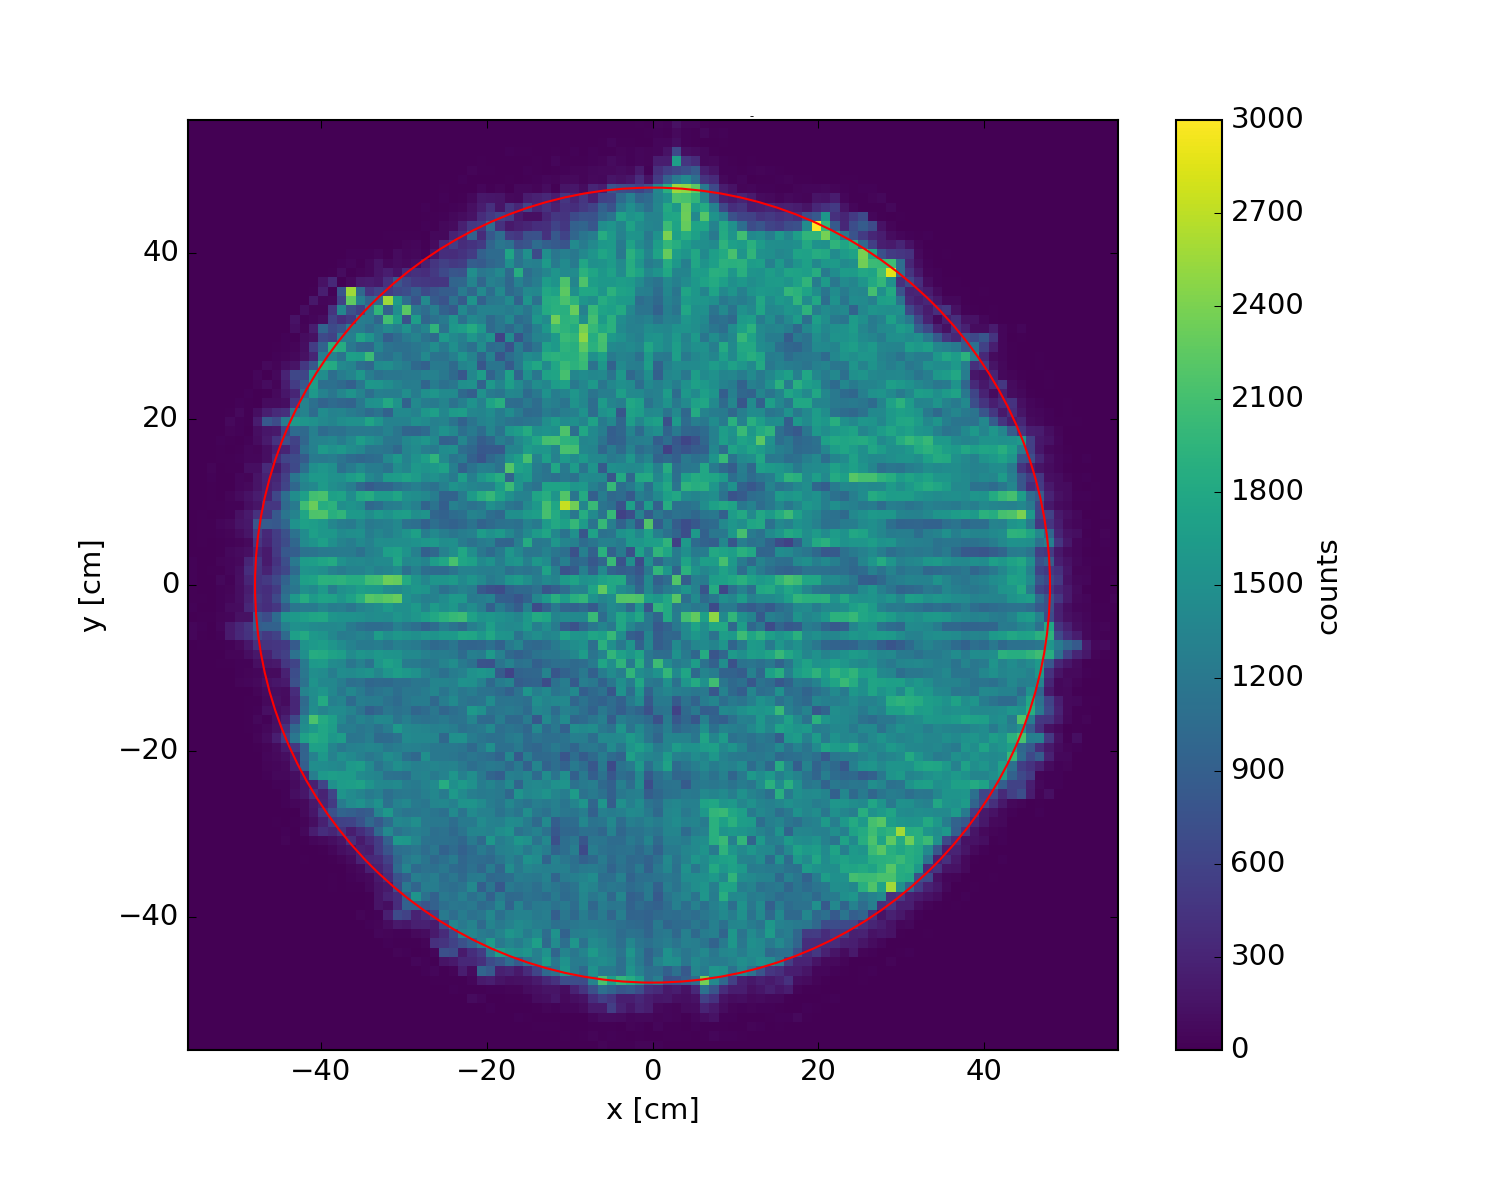
\includegraphics[width=0.555\textwidth]{xe1t_pos_rec_xy_kr}} \hfill
	\subfloat{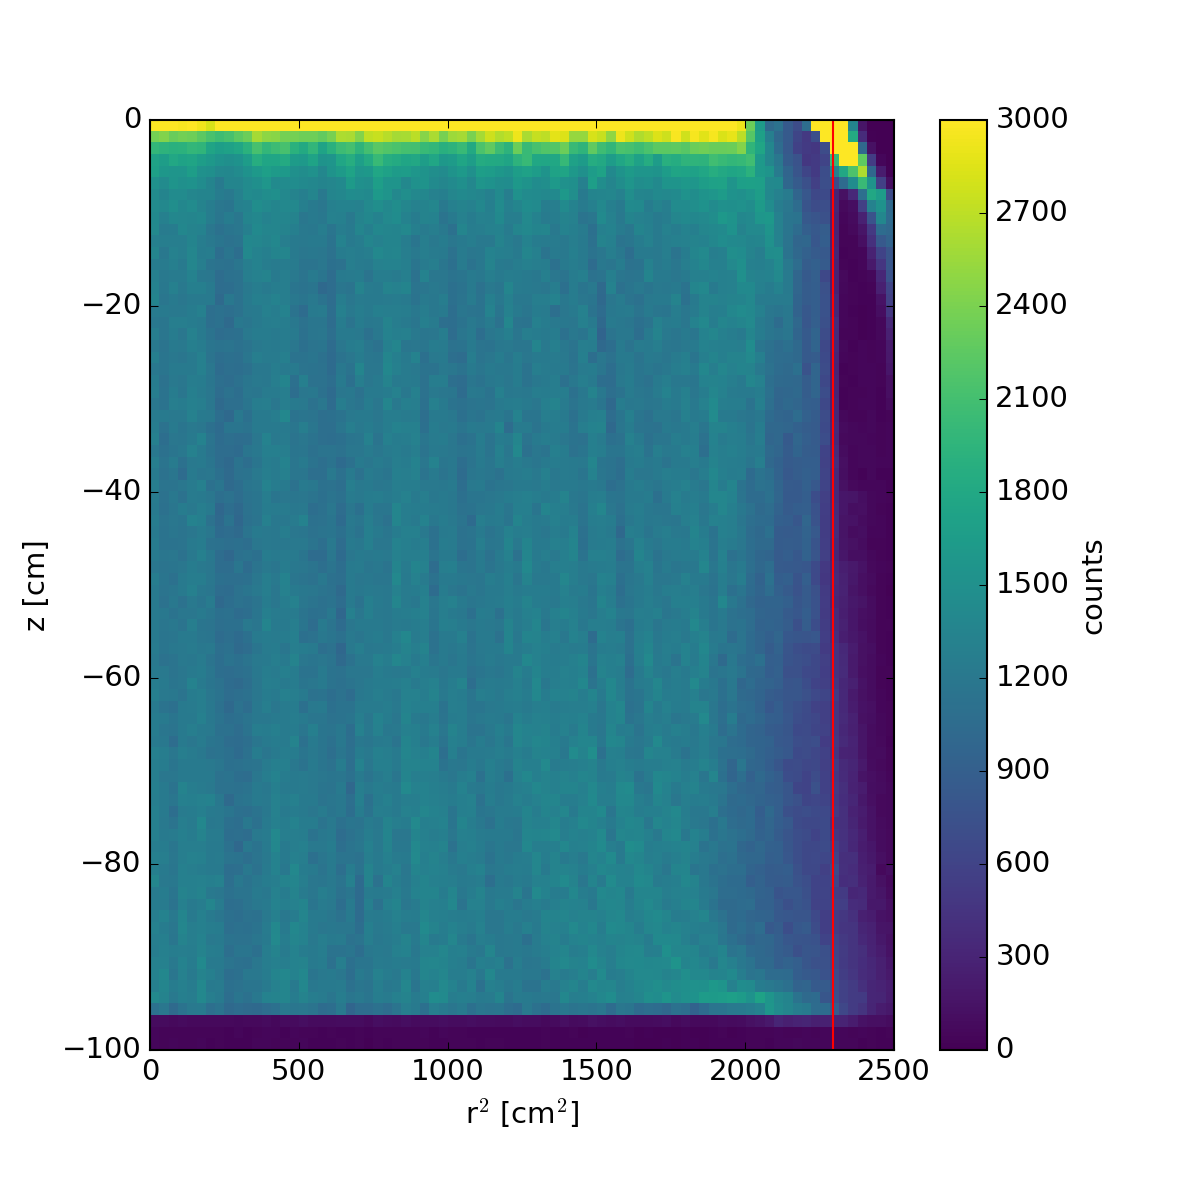
\includegraphics[width=0.445\textwidth]{xe1t_pos_rec_zr2_kr}}
	\caption{The distribution of positions of 32 keV events from \ce{^{83m}Kr} during the first science run of XENON1T.}
	\label{fig:xe1t_pos_rec_kr}
\end{figure}


\subsection{Position Dependent Corrections}
\label{sec:xe1t_pos_dependent_corrections}

\subsubsection{S1 Position Correction}
\label{sec:xe1t_lce_pos_correction}

One subtle, but critical, detector effect is the fact that the position of an event will affect the size of the S1 seen.  Understanding these losses as a function of position are critical to improve the resolution of the detector.  Fortunately, this S1 position dependence can be measured in a very simple way.  By introducing a source that will distribute throughout the entire detector and give a monoenergetic recoil, we can measure the difference in light yield for given positions.  Uniform sources are very useful this type of measurement but they are not necessary, especially for small detectors.

In XENON1T, the 32 keV emission of \ce{^{83m}Kr} was used to find the S1 correction map, which is shown in \figref{fig:xe1t_s1_correction_map}.  The decay of \ce{^{83m}Kr} not only creates a 32 keV electronic recoil but actually is followed by a second decay with a lifetime of 154 ns and energy of 9.4 keV.  This close time coincidence can be used to further confirm that only 32 keV events are being kept for the analysis.  This correction map, which shows the light yield at a given position relative to the average light yield in the detector, can then be used to correct recoils of all energies and types to improve the detector resolution.  While the correction map could be in three dimensions, since the TPC is cylindrically symmetric, we only correct in radial and depth coordinates.


\begin{figure}[t]
	\centering
	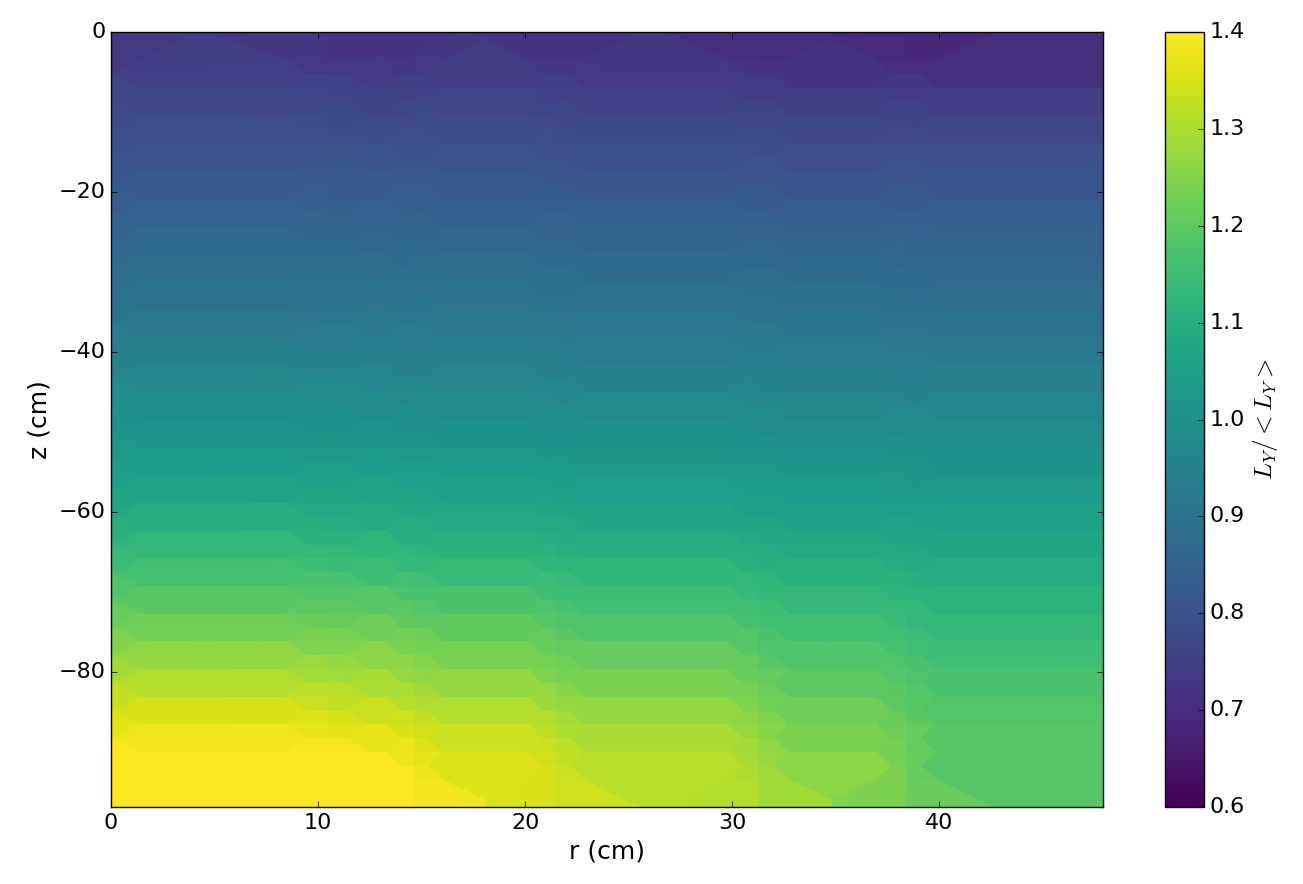
\includegraphics[width=0.99\textwidth]{xe1t_s1_correction_map}
	\caption{The S1 correction map of XENON1T.  This correction map shows the relative light yield of events at specific positions relative to the average light yield of the detector for monoenergetic events.  One can see the clear trend that events closer to the bottom PMT array have higher light yields than those closer to the liquid-gas interface.}
	\label{fig:xe1t_s1_correction_map}
\end{figure}


A clear trend can be seen in \figref{fig:xe1t_s1_correction_map}: the closer to the bottom PMT array an event is, the higher the light yield will be.  To a lesser extent, the closer the event is to the center of the detector, the higher the light yield will be.  This trend is related to the longer path length and larger number of reflections events towards the top and edge of the detector will have versus events very close to the bottom PMT array.

In theory, the position dependence of S1 could also be simulated but given the many factors that need to be understood and fed into the simulation, such as the absorption length and the Rayleigh scattering length in liquid xenon for 178 nm photons in liquid xenon, the reflectivity of the different materials, and the optical transparency of the meshes, this is impractical (especially given the simplicity of a direct measurement.


\subsubsection{S2 Transverse Position Correction}

In almost the same way that we can find the S1 correction map, we find S2 transverse position correction map.  However, instead of only using the 32 keV signal, we used the S2 of both the 32 keV and 9 keV decays (since they can only be resolved in S1 and not S2).  The correction maps for the top and bottom PMT arrays are shown in \figref{fig:xe1t_s2_correction_map_xy}.


\begin{figure}[t]
	\centering
	\subfloat{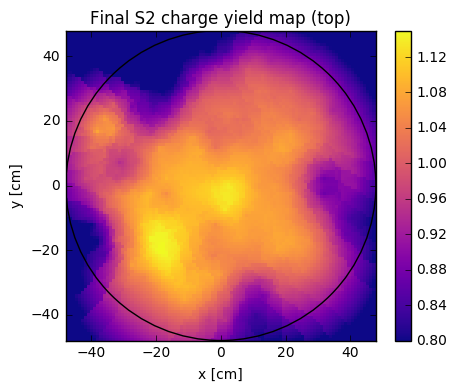
\includegraphics[width=0.5\textwidth]{xe1t_s2_correction_map_xy_top}} \hfill
	\subfloat{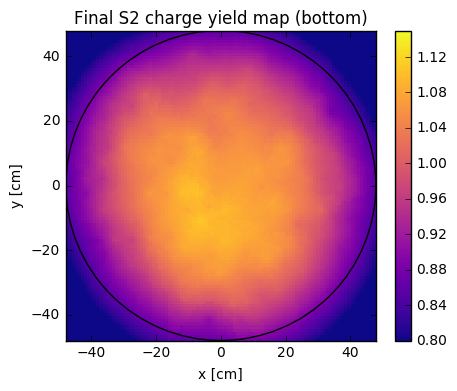
\includegraphics[width=0.5\textwidth]{xe1t_s2_correction_map_xy_bottom}}
	\caption{The S2 transverse position correction map of XENON1T.  This correction map shows the relative charge yield of events at specific positions relative to the average charge yield of the detector for monoenergetic events.  One can see the trend for the bottom PMT array that events closer to the center of the detector have higher charge yields than events closer to the edges.}
	\label{fig:xe1t_s2_correction_map_xy}
\end{figure}

As one can see, the correction maps look quite different.  This is mainly due to the close proximity of the S2 light to the top PMT array such that non-functional PMTs cause features in the map.  The S2 transverse position correction map for the bottom PMT array, on the other hand, is very smooth because the light must travel further and is less dependent on single PMT.  Ultimately, in the first science run, it was decided that only the bottom PMT array would be used for calculating signal sizes so only the smoother bottom PMT map was needed.

In the bottom PMT map, one can again see the trend that events towards the center of the detector have higher charge yields than events closer to the edge of the TPC.  This effect is believed to be from charge collecting on the teflon, edge effects for the electric field produced by the anode and the gate, and again from the longer path lengths and larger number of reflections for photons originating closer to the edge of the detector.


\subsubsection{S2 Depth Correction Correction: Electron Lifetime}

As mentioned in \secref{sec:tpc_s2_sig}, the free electrons extracted from the interaction site by the drift field can be absorbed by electronegative impurities contaminating the liquid xenon.  These impurities, mostly oxygen, will therefore decrease the size of the S2 signal measured.  It turns out that the probability that an electron successfully reaches the liquid-gas interface is well described by the fairly simply relationship shown in \eqnref{eqn:xe1t_electron_lifetime}.

\begin{equation}
        \label{eqn:xe1t_electron_lifetime}
        p_{\textrm{EL}}(z) = \frac{1}{\tau_{e^-}} e^{-\frac{z}{v_d \tau_{e}}}
\end{equation} 

Since the S2 signal size is directly proportional to the number of electrons accelerated through the gaseous xenon, \eqnref{eqn:xe1t_electron_lifetime} should manifest itself as an exponential decrease in the S2 size as a function of depth.  A plot of this effect can be seen in \figref{fig:xe1t_electron_lifetime}.


\begin{figure}[p]
	\centering
	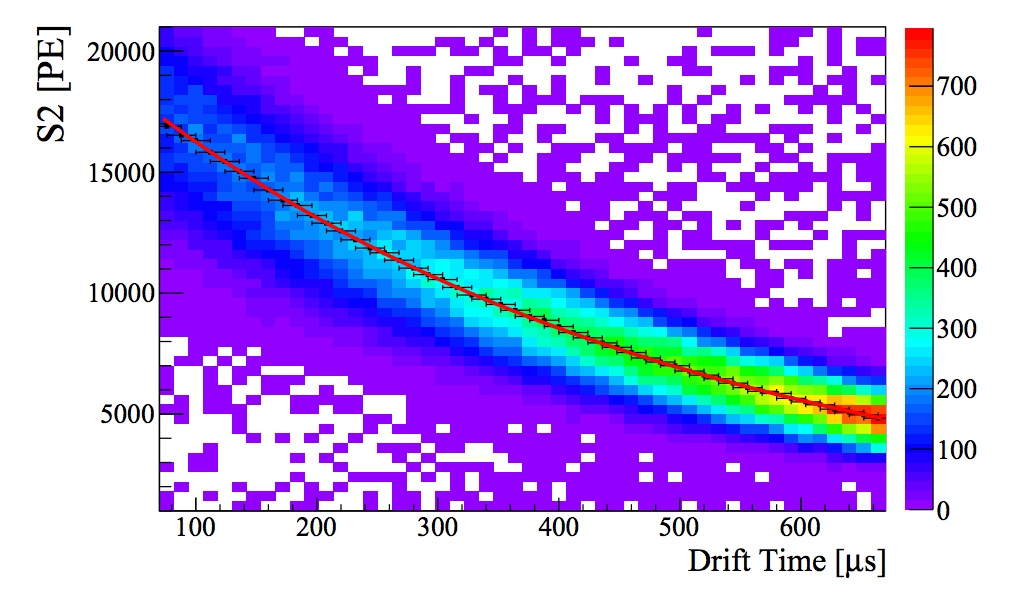
\includegraphics[width=0.99\textwidth]{../../Chapter2/images/tpc_electron_lifetime.jpeg}
	\caption{An example of an electron lifetime analysis from XENON1T.  In this analysis, the 41 keV \ce{^{83m}Kr} electronic recoil is used and the decay's S2 signal size is plotted versus drift time (a proxy for depth).  Image Credit: \citeref{aprile2017xenon1t}.}
	\label{fig:xe1t_electron_lifetime}
	
	\centering
	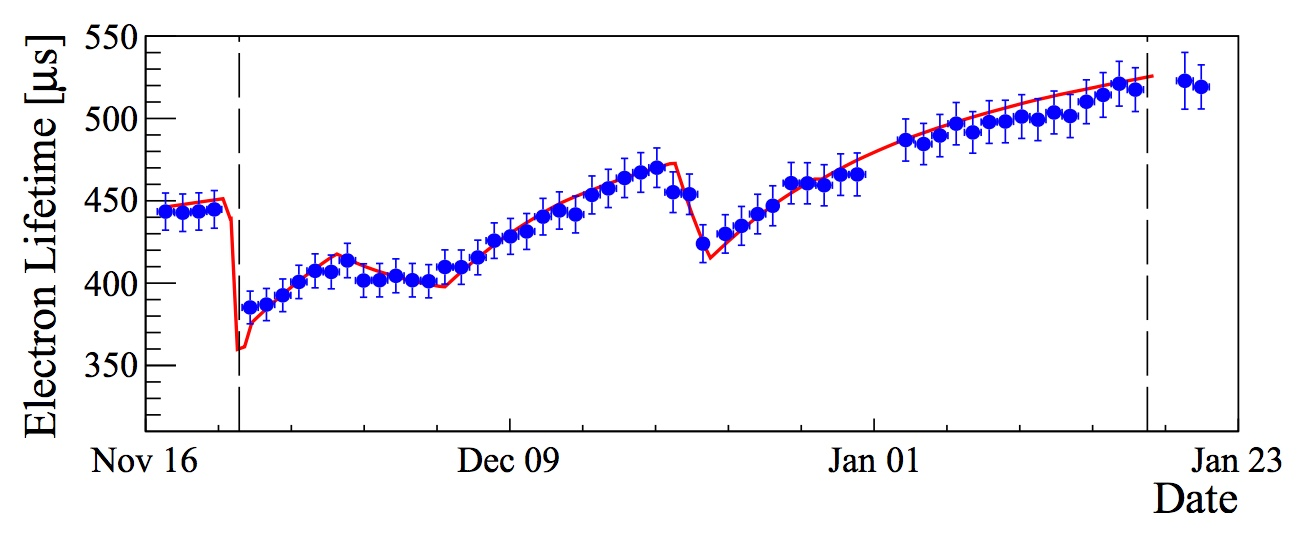
\includegraphics[width=0.99\textwidth]{xe1t_electron_lifetime_sr0}
	\caption{The electron lifetime over the course of the first science run of XENON1T.  Notice the two drops in the electron lifetime corresponding to periods when the purification system was not operating.  Shown in red is a prediction of the electron lifetime given the detector operating parameters and outgassing estimates from materials.  Image Credit: \citeref{aprile2017xenon1t}.}
	\label{fig:xe1t_electron_lifetime_sr0}
\end{figure}


Electronegative impurities emanate from the materials used to construct the detector and therefore are constantly introduced into the system.  Therefore, these impurities must constantly be cleaned out.  This cleaning also does not remove all impurities instantaneously --- the electron lifetime must be measured routinely in order to monitor its day-to-day changes.  These effects can be seen in \figref{fig:xe1t_electron_lifetime_sr0} which shows both drops from when the purification went offline and the steady increase in purity from continuous cleaning.


In XENON1T, this cleaning is done by the purification system described in \secref{sec:xe1t_pur_electronegative}.  Because the a low electron lifetime has an adverse impact on the S2 resolution (and hence energy resolution and discrimination power), significant effort has gone into and will continue to go into improving electronegative purification for large scale detectors.  


\subsection{Single Electron Gain}
\label{sec:xe1t_gas_gain}

The single electron gain, also referred to as \textit{gas gain}, is used to quantify the number of photons detected per electron extracted from the liquid into the gas phase.  While both the production of scintillation light from electrons exciting gaseous xenon atoms and the detection of scintillation photons are both well approximated by Poisson processes.  However, due to detector effects, such as the per PMT detection efficiency and variations in the field in the gaseous xenon, will cause further smearing of the number of photons detected from a single electron.  If we assume that this smearing is Gaussian, then we can actually fit the number of photons detected with a Poisson convolved with a Gaussian to determine the final probability mass function.  

An example of a fit of the gas gain is shown in \figref{fig:xe1t_single_electron_gain} where hits are found by looking at voltage excursions over threshold on a per-PMT basis in a time window defined by the waveform summed across all PMTs.

\begin{figure}[t]
	\centering
	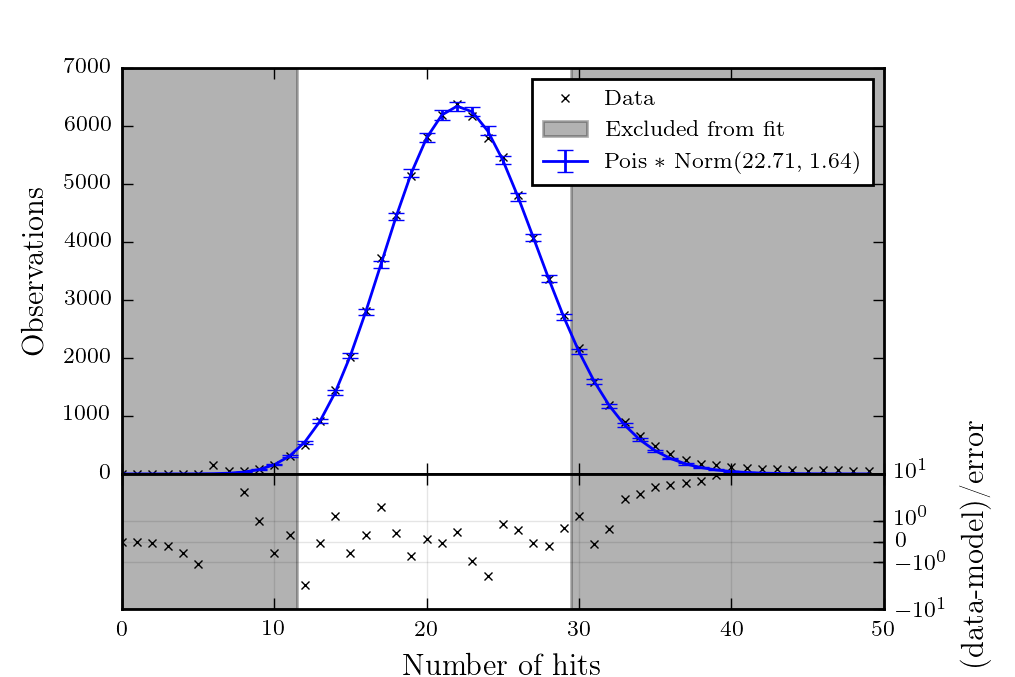
\includegraphics[width=0.99\textwidth]{xe1t_single_electron_gain}
	\caption{The fit single electron gain from the first science run of XENON1T.  Hits are defined as excursions above threshold for individual PMTs in a time window defined by the waveform summed across all PMTs.}
	\label{fig:xe1t_single_electron_gain}
\end{figure}


Since it is expected that the gas gain is sensitive to the electric field in the gas phase, the gas gain is susceptible to change with small changes in the liquid level.  Therefore, the gas gain is constantly monitored throughout data taking to ensure that it is stable.


\subsection{Average Light Collection Efficiency and Extraction Efficiency}
\label{sec:xe1t_anticorrelation}


In \secref{sec:lxe_er_observables}, we discussed the observables production process for electronic recoils and found a relationship between the energy of electron recoils and the number of photons and free electrons produced because of the lack of quenching factors in the observables production mechanism.  This relationship is shown in \eqnref{eqn:xe1t_anticorrelation} where $N_q$ is the number of quanta, $\textrm{E}_{\textrm{ER}}$ is the energy of the electronic recoil, $W$ is the average energy required to produce an exciton or electron-ion pair ($13.7 \pm 0.2$ eV \cite{dahl_thesis}), $N_{\gamma}$ is the number of photons produced in the electronic recoil, and $N_e$ is the number of free electrons extracted from the interaction site.

\begin{equation}
        \label{eqn:xe1t_anticorrelation}
        N_q = \frac{\textrm{E}_{\textrm{ER}}}{W} = N_{\gamma} + N_{e}
\end{equation}

While \eqnref{eqn:xe1t_anticorrelation} looks very simple, it actually proves to be very valuable when measuring two otherwise very difficult to measure/simulate detector parameters: the average light collection efficiency of photons and the extraction efficiency of electrons from the liquid into the gas.  

We can easily convert the number of photons and free electrons from the interaction into the observables measured by our detector, S1 and S2.  Since S1 is the number of photons detected, we say that $\textrm{S1} = N_{\gamma} \cdot g_1$, where $g_1$ is the average light collection efficiency.  The S2 signal is directly proportional to the number of electrons extracted from the liquid into the gaseous xenon.  Therefore, we can say that $\textrm{S2} = N_e g_2 = N_e \cdot G_e \eta$ where $G_e$ is the single electron gain (see \secref{sec:xe1t_gas_gain}) and $\eta$ is the efficiency of extracting electrons from the liquid into the gaseous xenon (often referred to as the \textit{extraction efficiency}).

  This allows us to put \eqnref{eqn:xe1t_anticorrelation} into terms of measured parameters.
  
\begin{equation}
        \label{eqn:xe1t_anticorrelation_s1_s2}
        \frac{\textrm{E}_{\textrm{ER}}}{W} = \frac{\textrm{S1}}{g_1} + \frac{\textrm{S2}}{G_e \eta}
\end{equation}
 
  \begin{figure}[t]
	\centering
	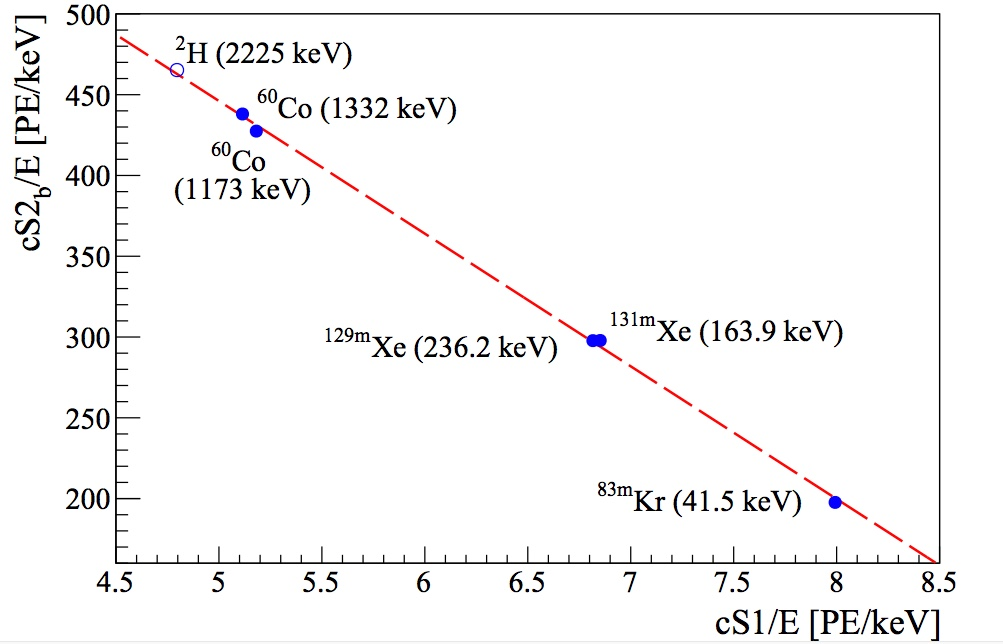
\includegraphics[width=0.95\textwidth]{xe1t_doke_plot}
	\caption{The Doke plot for XENON1T along with the best fit.  Note that only the bottom PMT array is used for the S2 signal and that we use the position corrected values of S1 and S2.  While the de-excitation from neutron captures in water is shown (\ce{^{2}H} with an de-excitation energy of 2.225 MeV), it is not used for the fit.}
	\label{fig:xe1t_doke_plot}
\end{figure}

 
We can now look at multiple monoenergetic peaks or the same monoenergetic peak at different electric fields (or multiple monoenergetic peaks at multiple electric fields).  A simple rearrangement of \eqnref{eqn:xe1t_anticorrelation_s1_s2} shows us that the S1 and S2 values of these peaks should fall along a line defined by $g_1$, $\eta$, and $G_e$.

 \begin{equation}
        \label{eqn:xe1t_anticorrelation_line}
        \frac{\textrm{S2}}{\textrm{E}_{\textrm{ER}}} = \frac{G_e \eta}{g_1} \frac{\textrm{S1}}{\textrm{E}_{\textrm{ER}}} - \frac{G_e \eta}{W}
\end{equation}
 
 We can fit what is colloquially referred to as a \textit{Doke plot} (after Tadayoshi Doke) with the mean S1 and S2s of various monoenergetic electronic recoils (potentially at different fields) using \eqnref{eqn:xe1t_anticorrelation_line} in order to extract $g_1$ and $eta$.  Note that $eta$ can only be extracted if one independently measures the single electron gain since otherwise the two parameters will be completely correlated.  The fit of multiple monoenergetic electronic recoils to find the extraction efficiency and the average light collection efficiency of XENON1T is shown in \figref{fig:xe1t_doke_plot}. 
 
 

\subsection{Cut Acceptance}
\label{sec:xe1t_cut_acceptance}

\begin{figure}[t]
	\centering
	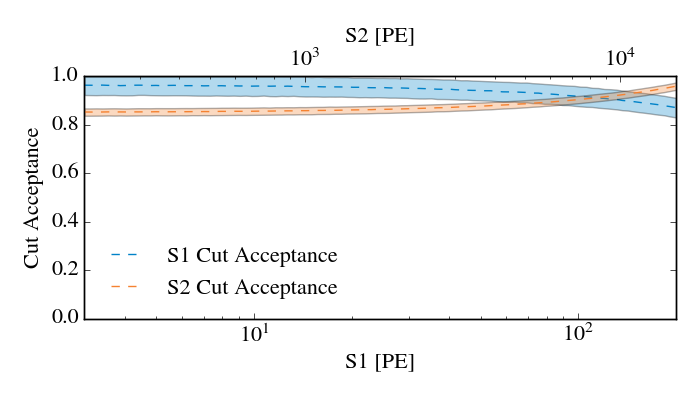
\includegraphics[width=0.99\textwidth]{xe1t_cut_acceptances}
	\caption{The estimated cut acceptances in S1 and S2 for the first science run of XENON1T.}
	\label{fig:xe1t_cut_acceptances}
\end{figure}


Cuts in XENON1T are used to eliminate background sources, like the fiducial volume cut and the single scatter cuts, or to remove events that show non-standard behavior, such as the S2 width cut that uses the diffusion model to define appropriate widths given a drift time (this relationship between drift time and width can actually be seen in \figref{fig:xe1t_drift_time_vs_width}).  Once the cuts are in place, it is important to understand the population of good events that are removed as a function of signal size --- this is referred to as the \textit{cut acceptance}.  

To define the cut acceptance, we use the ``N-1'' approximation.  The N-1 approximation calls for applying all but a single one of the cuts to define the control sample which is then compared to the sample after applying the final cut.  It is important to note that this does not account for potential correlations between cuts.  Using the N-1 approximation for each of the cuts and combining the individual acceptances, we can find the overall cut acceptance of the first science run of XENON1T as a function of S1 and S2 (shown in \figref{fig:xe1t_cut_acceptances}).

It is important to note that, with a sufficiently trust-worthy physics and detector simulator, one could estimate the cut acceptances using simulation. 




\section{Electronic and Nuclear Recoil Characterization of XENON1T}
\label{sec:xe1t_er_nr_calibration}

The electronic and nuclear recoil calibrations are two of the most important studies required for a liquid xenon TPC.  For the first time in xenon detectors, these calibrations were performed such that a realistic approximation of the microphysics process was accounted for alongside the detector effects discussed.  This was only made possible with the use of a fast Monte Carlo (MC) framework that was developed by the author and discussed in the next chapter that leveraged graphical processing units (GPUs) for dramatic increases in speed (two to three orders of magnitudes).

While these calibrations can (and in future science runs will be) performed together due to the large number of shared parameters, in the first science run of XENON1T they were performed separately.  


\subsection{Significance of the Calibrations}

Before discussing the details of the calibrations, it is helpful to understand why these calibrations are of such high importance.  Ultimately, the goal of each science run is to search for a WIMP signal in the detector.  While this can be done in a purely statistical fashion (as discussed in \secref{sec:dm_direct_detection}), more sophisticated methods have been developed that drastically improve the sensitivity of TPCs to WIMPs.  

Since the background in XENON1T is thoroughly understood, as outlined in \secref{sec:xe1t_er_bkg} and \secref{sec:xe1t_er_bkg}, we can actually create a probability distribution function (PDF) in our signal space (S1 and S2 space or some variation of this) \textit{if} our calibration captures the various processes between energy deposition all the way to signal extraction by the processor.  This probability distribution function can be made with WIMPs (or other dark matter candidates) to determine whether or not the data agrees with a WIMP of a given mass and cross section.  Determining how well WIMPs of given masses and cross sections agree with the data ultimately determines the limit set (if all WIMPs below a given cross section agree with the data) or whether a discovery was made (if the data favors a particular mass and cross section more than all others).

\begin{figure}
        \centering
	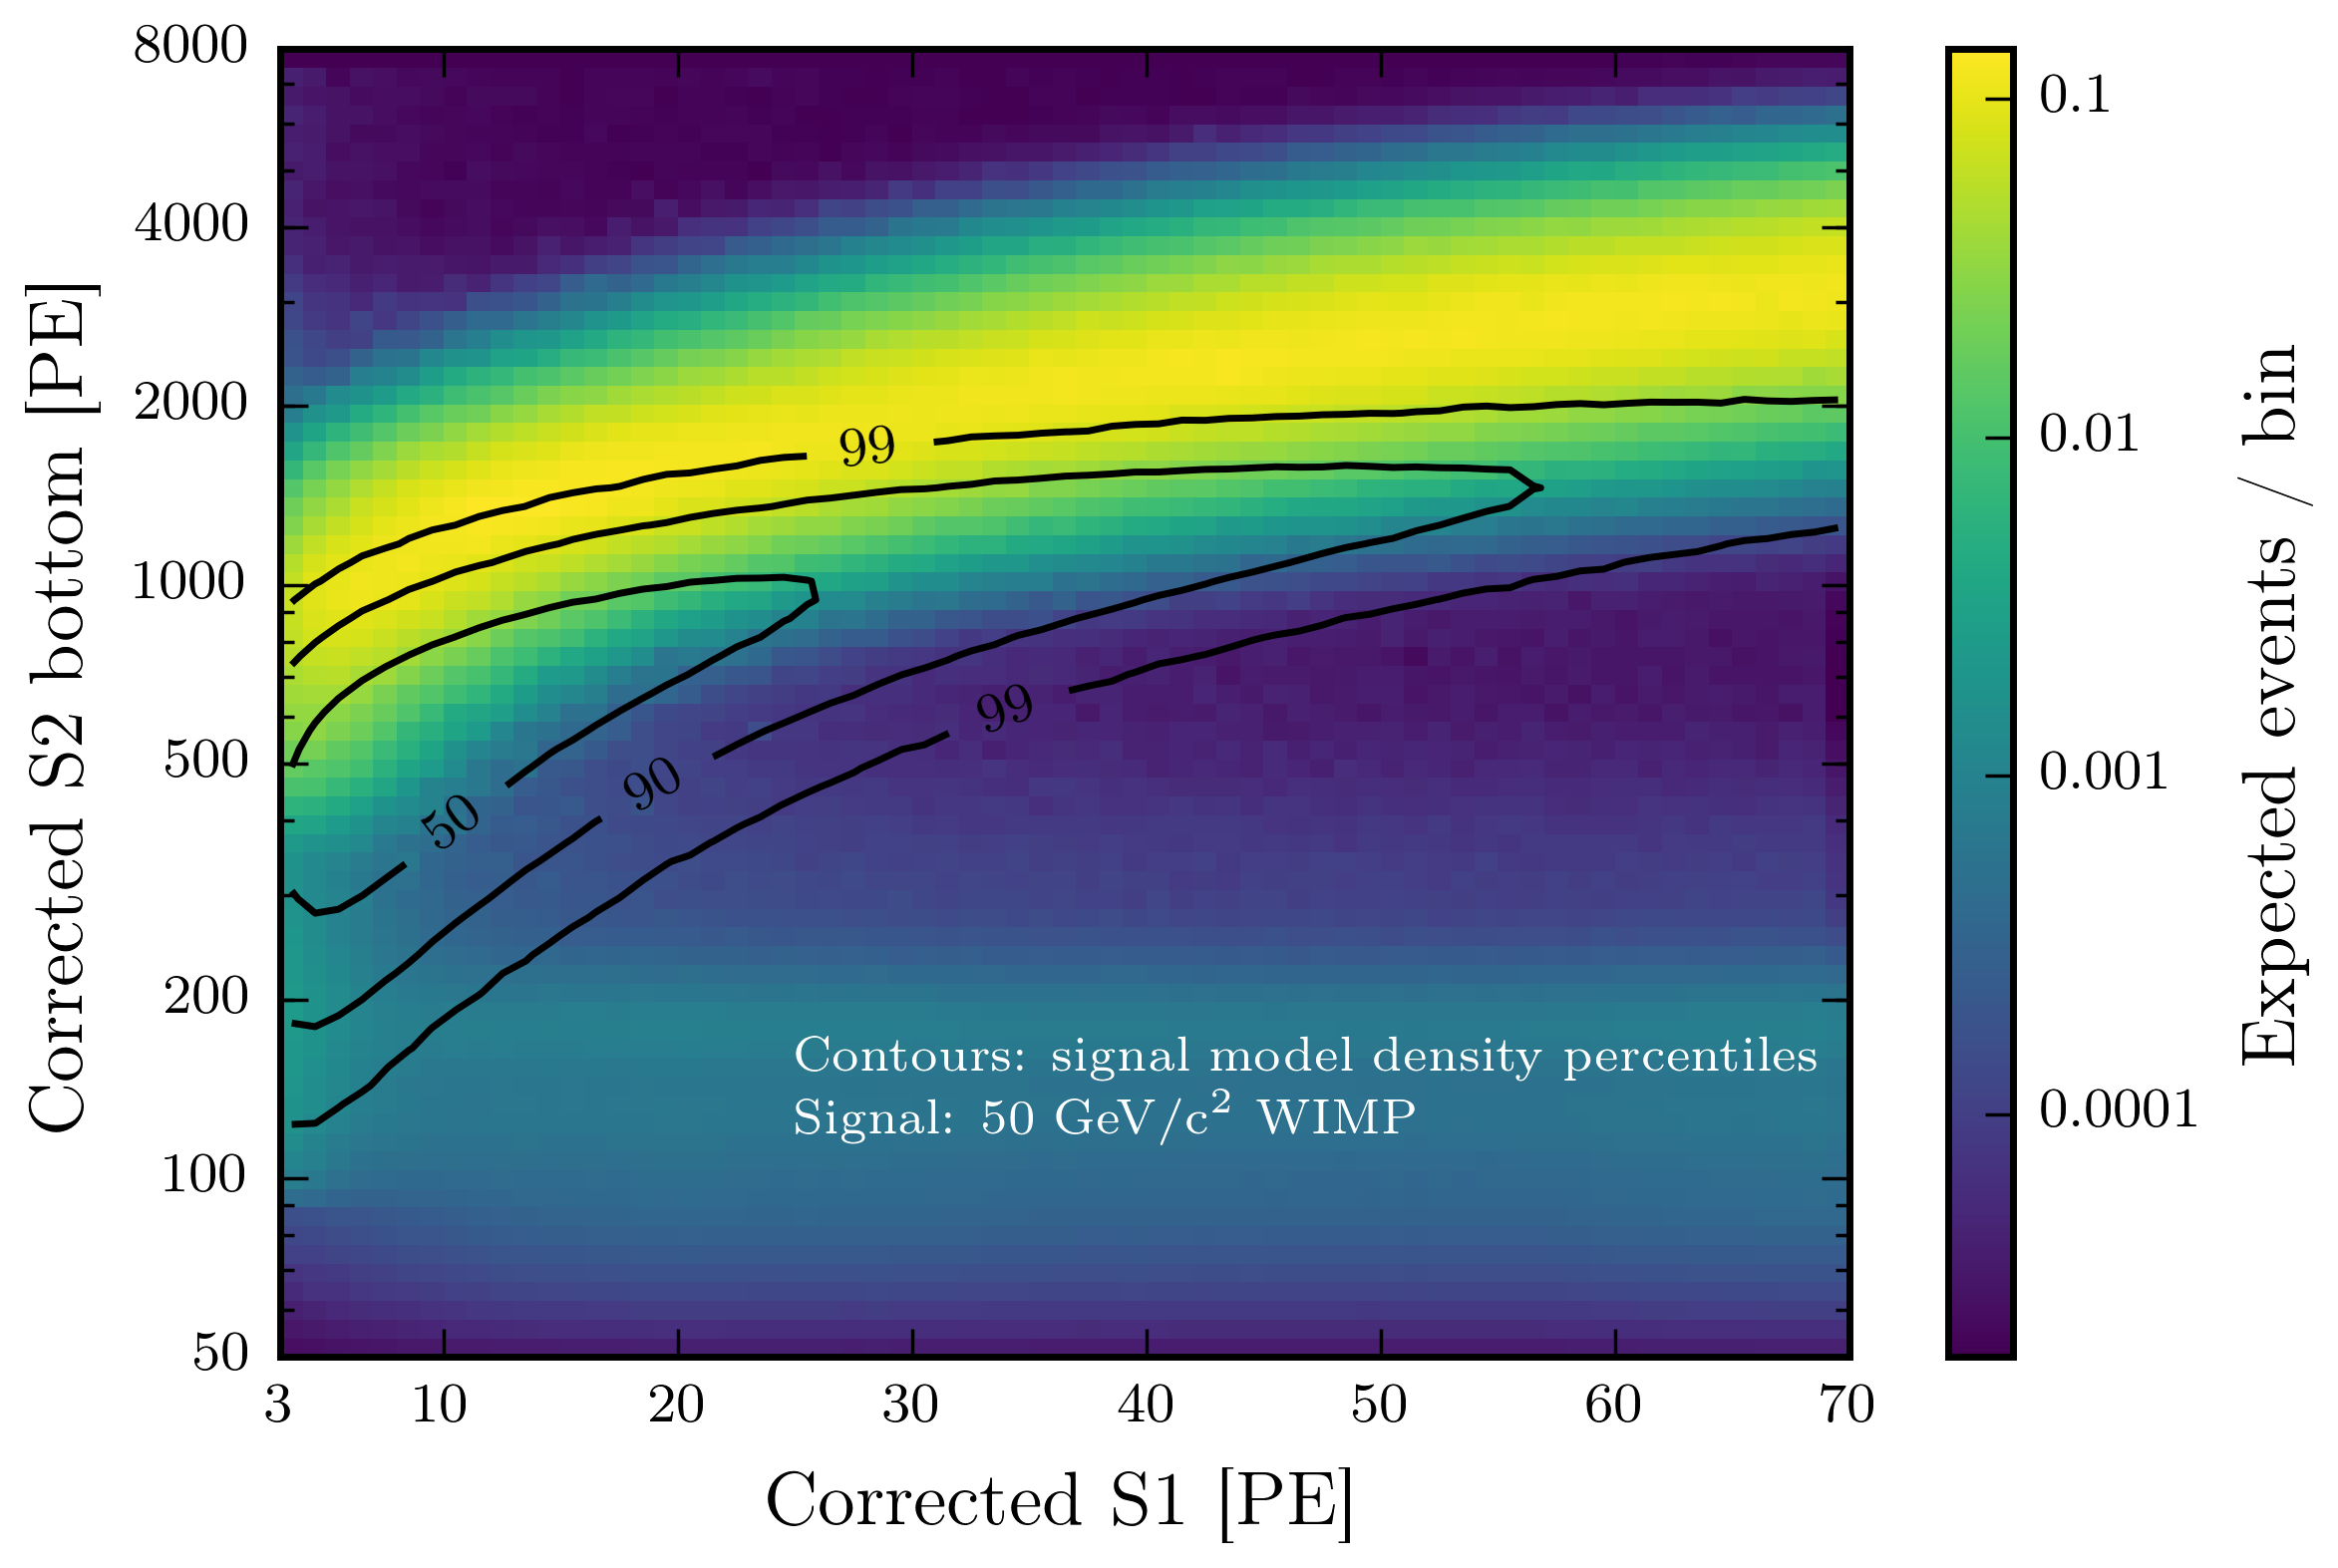
\includegraphics[width=0.99\textwidth]{xe1t_background_pdf}
	\caption{The probability distribution function for the first science run of XENON1T plotted with the cumulative density contours of a 50 $\sfrac{\textrm{GeV}}{\textrm{c}^2}$ WIMP.  The combined signal and  background PDF is used to either set a limit on the WIMP mass and cross section or claim a discovery.}
	\label{fig:xe1t_background_pdf}
\end{figure}

\figref{fig:xe1t_background_pdf} shows the PDF of the background distribution for the first science run with the cumulative density contours of a 50 $\sfrac{\textrm{GeV}}{\textrm{c}^2}$ WIMP.  These PDF and contours were made using the signal production models that were measured via the electronic and nuclear recoil calibrations.



\subsection{Parameter Estimation via Monte Carlo}


\begin{figure}
        \centering
	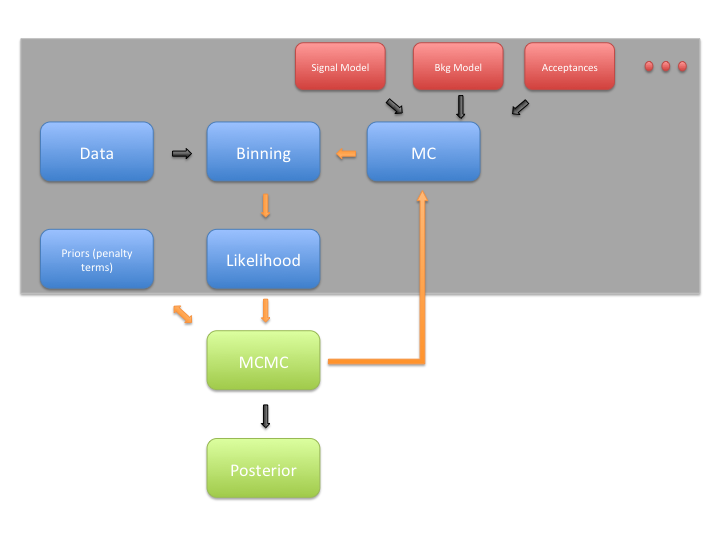
\includegraphics[width=0.99\textwidth]{xe1t_fast_mc_flowchart}
	\caption{A flowchart summarizing how a fast Monte Carlo is used to estimate the parameters in the signal production model.  Orange steps are done in each iteration of the parameter estimation where as black arrows represent steps that are only done a single time.}
	\label{fig:xe1t_fast_mc_flowchart}
\end{figure}


\figref{fig:xe1t_fast_mc_flowchart} shows a flowchart that summarizes how the calibration of electronic and nuclear recoils is performed.  The main idea is that a detailed Monte Carlo is used to estimate the expected distribution of events in signal space (S1 and S2 for XENON1T), which can then be compared to the actual measured distribution of events to determine what values for the parameter model cause the highest level of agreement. 

In more technical terms, the Monte Carlo is used to create a PDF which is then compared with data which results in a likelihood.  This likelihood can be combined with prior distributions of the model parameters (from previous measurements or calibrations).  As you vary the parameters in the signal production model, you would expect this likelihood to increase and decrease.  One can then use different algorithms to find either the set of parameters best in agreement with the data (via a minimizer) or the posterior distribution of the parameters (via a Markov Chain Monte Carlo or MCMC).

The benefit to using a Monte Carlo to define a likelihood for parameter estimation is that your signal production model can be arbitrarily complex.  The downside of using a MC to estimate your likelihood is that it is extremely inefficient, typically rendering this approach impractical.  However, using graphical processing units, the author was able to develop an analysis framework that made this type of analysis feasible.  The details of the framework will be discussed in detail in the next chapter.

The details of Monte Carlo event production will be discussed in \secref{sec:xe1t_mc_observables_production_er}, \secref{sec:xe1t_mc_observables_production_nr}, and \secref{sec:xe1t_mc_detector}.  These Monte Carlo events are used to fill a histogram that is compared with a histogram filled with data via a binned likelihood, which will be discussed in \secref{sec:xe1t_mc_likelihood}.  In this way we can quantify how well a given set of parameters agrees with what we have measured.  The set of parameters to be tested is chosen in this analysis by a Markov Chain Monte Carlo (MCMC) but realistically could be done with most parameter estimation algorithms --- we will briefly discuss how the posterior probability space of the parameters was calculated in \secref{sec:xe1t_mcmc}.
 

\subsubsection{Light and Charge Production for Electronic Recoils}
\label{sec:xe1t_mc_observables_production_er}

The details of the light and charge production model for electronic recoils are very similar to the details from the calibration discussed in \citeref{aprile2017tritium}.  

Given an electronic recoil of a known energy, the first quantity of interest is the number of quanta produced in the interaction.  For electronic recoils, this is approximated as a Fano process as shown in \eqnref{eqn:xe1t_er_fano}.

\begin{equation}
        \label{eqn:xe1t_er_fano}
        N_q \sim N \left( \mu = \frac{E}{W}, \sigma^2 = \frac{F E}{W} \right) 
\end{equation}

The Fano factor in liquid xenon is estimated to be 0.059 eV \cite{doke1976estimation} and was fixed during parameter estiamtion.  Since little quenching is expected for electronic recoils in liquid xenon, these quanta can take the form of only excitons and electron-ion pairs.   To simulate the individual number of excitons and ions, we use a binomial process with a probability defined by the \textit{exciton-to-ion} ratio.


\begin{equation}
        \label{eqn:xe1t_er_exciton_ion}
        N_{\textrm{ion}} \sim B \left( N=N_q, p = \frac{1}{1 + \frac{N_{\textrm{ex}}}{N_{\textrm{ion}}}} \right) , \, \, \, N_{\textrm{ex}} = N_q - N_{\textrm{ion}}
\end{equation}


We now must consider the possibility of electron-ion pairs recombining to form excitons, resulting in a single photon rather an electron extracted from the site.  The recombination fraction $r$ depends on the energy and field present in the liquid and it has a non-negligible intrinsic recombination fluctuation $\Delta r$ \cite{akerib2016tritium, aprile2017tritium}.  It is assumed that the recombination is normally distributed as shown in \eqnref{eqn:xe1t_recombination_fluc}

\begin{equation}
        \label{eqn:xe1t_recombination_fluc}
        r \sim N(\mu = \left< r \right>, \sigma^2 = (\Delta r)^2)
\end{equation}

We then approximate the recombination of electron-ion pairs as a binomial process as shown in \eqnref{eqn:xe1t_recombination}.

\begin{equation}
        \label{eqn:xe1t_recombination}
        \begin{gathered}
                N_{\textrm{rec}} \sim B(N = N_{\textrm{ion}}, p = r), \\ 
                N_{\textrm{ion}} \leftarrow N_{\textrm{ion}} - N_{\textrm{rec}}, \, \, \,  N_{\textrm{ex}} \leftarrow N_{\textrm{ex}} + N_{\textrm{rec}}
        \end{gathered}
\end{equation}


Recombination was only considered above a certain energy threshold $E_t$.  

In total, eight free parameters were included in the observables production model: five from the fourth-order polynomial used to describe the light yield relative to a reference curve, one from the energy threshold for recombination (below which recombination no longer is considered), and two for the parameterization of the recombination fluctuation ($\Delta r = A \cdot (1 - e^{\sfrac{E}{\tau_r}})$).  A normal prior was assumed for $W$ with a mean of 13.7 eV and width of 0.2 eV while a uniform prior between 0.06 to 0.20 \cite{takahashi1975average, aprile2007observation} was assumed for the exciton-to-ion ratio due to the discrepancy between measured values.  

%, and a final parameter to describe a flat background in $\textrm{log}_{10} \left( \frac{\textrm{S2}}{\textrm{S1}} \right)$ versus S1 space.  


Since the electronic recoil calibration was performed with \ce{^{220}Rn}, a flat energy spectrum between 0--30 keV was used to draw the input energy for each Monte Carlo iteration.  Additionally, it was assumed that events occurred uniformly throughout the detector.



\subsubsection{Light and Charge Production for Nuclear Recoils}
\label{sec:xe1t_mc_observables_production_nr}

If you recall from \secref{sec:xe_nr_observables}, unlike electronic recoils, nuclear recoils will also lose energy due to atomic motion that can ultimately not be detected in a liquid xenon TPC.  We model this loss using Lindhard theory, which gives the energy lost to atomic motion as a function of energy.  This is shown in \eqnref{eqn:xe1t_lindhard} in terms of the dimensionless energy $\epsilon$.

\begin{equation}
        \label{eqn:xe1t_lindhard}
        \begin{gathered}
                \epsilon = 11.5 \left( \frac{E}{\textrm{keV}} \right) Z^{\sfrac{-7}{3}}, \\
                L(\epsilon) = \frac{k g(\epsilon)}{1 + k g(\epsilon)}, \, \, \, g(\epsilon) = 3 \epsilon^{0.15} + 0.7 \epsilon^{0.6} + \epsilon
        \end{gathered}
\end{equation}

The Lindhard factor, $L$, is then used to approximate the number of quanta as shown in \eqnref{eqn:xe1t_nr_quanta}.

\begin{equation}
        \label{eqn:xe1t_nr_quanta}
        N_q \sim P \left( \mu = \frac{E \cdot L}{W} \right)
\end{equation}

Note that the choice of the Poisson distribution is an approximation and not derived from first principles.  The actual distribution is likely more complicated due to complex track structure of nuclear recoils in liquid xenon.

Once we have the number of quanta, we can find the number of excitons and electron-ion pairs in the same way that we did for electronic recoils.

\begin{equation}
        \label{eqn:xe1t_nr_exciton_ion}
        N_{\textrm{ion}} \sim B \left( N=N_q, p = \frac{1}{1 + \frac{N_{\textrm{ex}}}{N_{\textrm{ion}}}} \right) , \, \, \, N_{\textrm{ex}} = N_q - N_{\textrm{ion}}
\end{equation}


We also must consider the recombination of electron-ion pairs for nuclear recoils.  Unlike electronic recoils, though, recombination fluctuations have not been observed for nuclear recoils.

\begin{equation}
        \label{eqn:xe1t_nr_recombination}
        \begin{gathered}
                N_{\textrm{rec}} \sim B(N = N_{\textrm{ion}}, p = r), \\ 
                N_{\textrm{ion}} \leftarrow N_{\textrm{ion}} - N_{\textrm{rec}}, \, \, \,  N_{\textrm{ex}} \leftarrow N_{\textrm{ex}} + N_{\textrm{rec}}
        \end{gathered}
\end{equation}

Given the small track size of nuclear recoils, we approximate that the recombination is described by the Thomas-Imel model \cite{thomas1987recombination} as defined in \eqnref{eqn:xe1t_ti_model}.


\begin{equation}
        \label{eqn:xe1t_ti_model}
        r = 1 - \frac{\textrm{ln}(1 + N_{\textrm{ion}} \sigma)}{N_{\textrm{ion}} \sigma}
\end{equation}


Finally, we must consider biexcitonic quenching, which results from the collision of two excitons.  This quenching is typically parameterized using the quenching term from Birks' saturation law, as shown in \eqnref{eqn:birks_quenching}, since one would expect that the density of excitons in a track to be proportional to the electronic stopping power \cite{mei2008model, tretyak2010semi, bezrukov2011interplay}. 

\begin{equation}
        \label{eqn:birks_quenching}
        f_B = \frac{1}{1 + a \frac{dE}{dx}} = \frac{1}{1 + \eta \epsilon^{- \lambda}}
\end{equation}


We then approximate that the number of excitons quenched is given by \eqnref{eqn:xe1t_biexcitonic_quenching}.

\begin{equation}
        \label{eqn:xe1t_biexcitonic_quenching}
        \begin{gathered}
                N_{\textrm{bq}} = B(N=N_{\textrm{ex}}, p = f_B), \\
                N_{\textrm{ex}} \leftarrow N_{\textrm{ex}} - N_{\textrm{bq}}
        \end{gathered}
\end{equation}


Note that we are assuming that the biexcitonic quenching process is binomial and that this is not from first principles.  There is also no requirement that excitons are quenched in pairs.  However, this quenching only is relevant at high energies so the effect from this approximation will be small\footnote{At high energies ($> 50$ keV) we will expect hundreds to thousands of excitons after recombination meaning the effect will be sub-1\%}.

\begin{figure}[t]
        \centering
	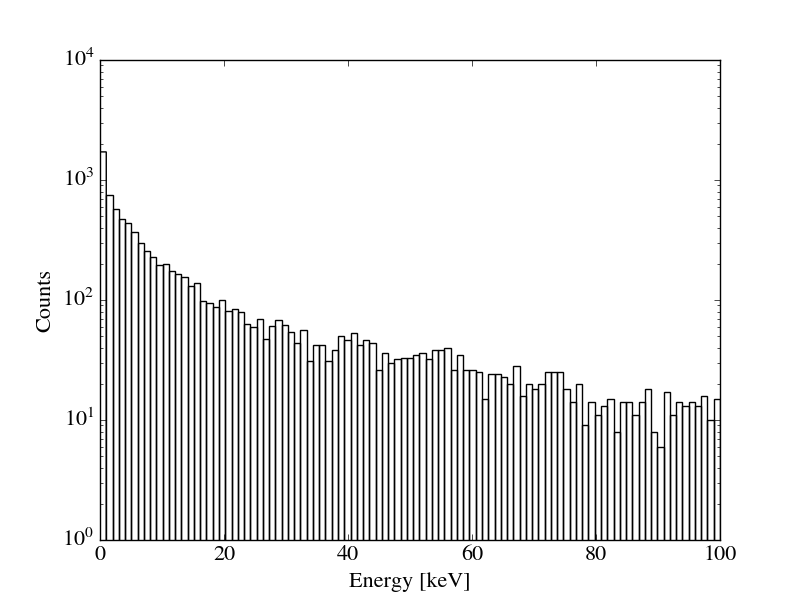
\includegraphics[width=0.99\textwidth]{xe1t_nr_energy_spec}
	\caption{The energy spectrum of single scatter and unresolvable multiple scatter nuclear recoils from the americium-beryllium (AmBe) source located in the water tank as predicted by Geant4.}
	\label{fig:xe1t_nr_energy_spec}
\end{figure}


The nuclear recoil data that was used for the calibration was from an americium-beryllium (AmBe) source, which produces neutrons of energies below 11 MeV.  The expected energy spectrum of single scatters in the medium (or multiple scatters that cannot be resolved in XENON1T due to their close proximity) from AmBe is shown in \figref{fig:xe1t_nr_energy_spec}.  Unlike the electronic recoil calibration, the expected distribution of positions of nuclear recoils in the detector is not expected to be uniform since the AmBe source produces neutrons outside the TPC.  The expected maps of location of nuclear recoils are shown in \figref{fig:xe1t_nr_positions}.  The energy spectra and interaction positions were extracted from a detailed Monte Carlo simulation produced in Geant4 \cite{agostinelli2003geant4}.



\begin{figure}[t]
        \centering
	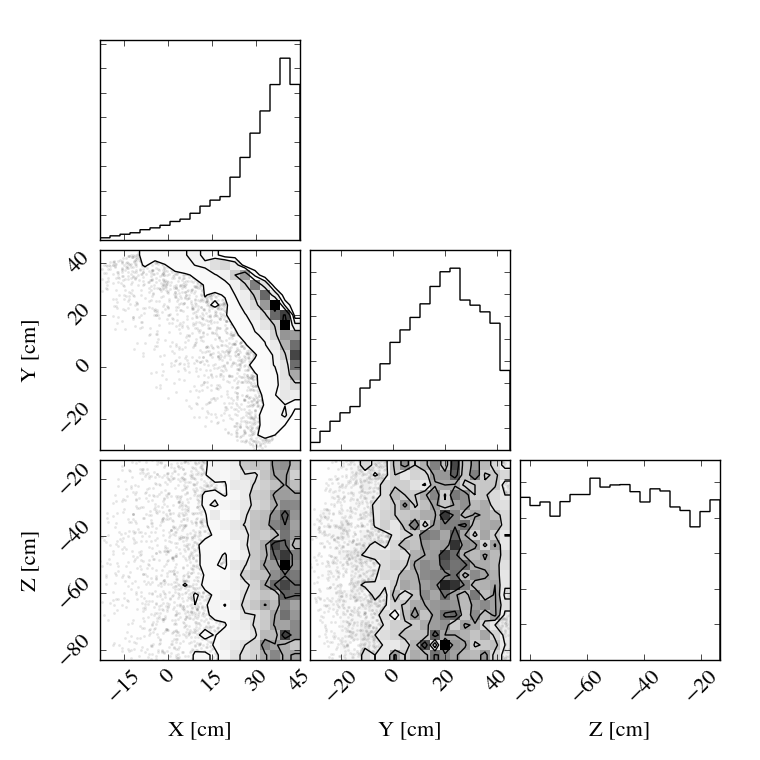
\includegraphics[width=0.99\textwidth]{xe1t_nr_positions}
	\caption{The location of single scatter and unresolvable multiple scatter nuclear recoils from the americium-beryllium (AmBe) source located in the water tank as predicted by Geant4.}
	\label{fig:xe1t_nr_positions}
\end{figure}


It was decided to constrain the response model of liquid xenon to nuclear recoils described in this section using previous measurements of the light and charge yield in place of performing an independent measurement like the one performed in XENON100 \cite{aprile2013response}.  While the featureless energy spectrum played a large role in this decision, ultimately this decision was made so that we could conclusively demonstrate an understanding of the XENON1T detector.  If the response model had been left free, discrepancies and issues in the detector model could be made up through changes to the liquid xenon response model.  

To constrain the the liquid xenon response model for nuclear recoils, we used the global analysis performed in \citeref{lenardo2015global}.  \citeref{lenardo2015global} examined past independent measurements of the light and charge yield of nuclear recoils and fit the model described in this section to the final yields each of those measurements presented.  While no previous measurements used in \citeref{lenardo2015global} were performed that simultaneously measured the light and charge yield, all of the independent measurements of light and charge yield were used simultaneously in \citeref{lenardo2015global} to fit the model in an attempt to account for correlations.  

Ultimately, eight free parameters are used to describe the mean light and charge yield in liquid xenon in \citeref{lenardo2015global}.  $k$, $\eta$, and $lambda$ from \eqnref{eqn:xe1t_lindhard} and \eqnref{eqn:birks_quenching} are left free in the model.  Additionally, $\alpha$, $\zeta$, $\beta$, $\gamma$, and $\delta$ are introduced to parameterize the exciton-to-ion ratio and Thomas-Imel model as shown in \eqnref{eqn:xe1t_ex_ion_parameterization} and \eqnref{eqn:ti_model_parameterization}, respectively.


\begin{equation}
        \label{eqn:xe1t_ex_ion_parameterization}
        \frac{N_{\textrm{ex}}}{N_{\textrm{ion}}} = \alpha F^{-\zeta} (1 - e^{-\beta \epsilon})
\end{equation}

\begin{equation}
        \label{eqn:ti_model_parameterization}
        \sigma = \gamma F^{-\delta}
\end{equation}

\begin{table}[t]
\centering
\def\arraystretch{1.3}
\begin{tabular}{|c|c|}
\hline
Parameter & Result \\
\hline
$\alpha$ & $1.240^{+0.079}_{-0.073}$ \\ \hline
$\zeta$ & $0.0472^{+0.0088}_{-0.0073}$ \\ \hline
$\beta$ & $239^{+28}_{-8.8}$ \\ \hline
$\gamma$ & $0.01385^{+0.00058}_{-0.00073}$ \\ \hline
$\delta$ & $0.0620^{+0.0056}_{-0.0064}$ \\ \hline
$k$ & $0.1394^{+0.0032}_{-0.0026}$ \\ \hline
$\eta$ & $3.3^{+5.3}_{-0.7}$ \\ \hline
$\lambda$ & $1.14^{+0.45}_{-0.09}$ \\ \hline
\end{tabular}
\caption{The results of the fit from \citeref{lenardo2015global} of the nuclear recoil response model to independent measurements of the light and charge yield.}
\label{tab:xe1t_nest_results}
\end{table}

The results of the fit are shown in \tabref{tab:xe1t_nest_results}.  These results were used to set prior likelihoods for the nuclear recoil calibration\footnote{An asymmetric gaussian is used with widths defined by the asymmetric uncertainties of each parameter.} --- in this way, the data from XENON1T could be used to further constrain the model and results presented in \citeref{lenardo2015global}.  It is important to note that the results of the calibration do not constitute an independent measurement like the ones used to fit the model in \citeref{lenardo2015global}. 


\subsubsection{Detector Model for Signal Production}
\label{sec:xe1t_mc_detector}

Having discussed the light and charge production models for electronic and nuclear recoils, we can move onto how the S1 and S2 signals are produced from the light and charge.  While the detector processes will be the same for both the electronic and nuclear recoil calibrations, the parameters used to describe these properties will sometimes be different since the calibrations were performed at different times (e.g., the electron lifetime).


%\subsubsection{Position Dependence of Signals}

%In \secref{sec:xe1t_pos_dependent_corrections}, we discussed the ways in which our S1 and S2 can vary based on the location of the interaction in the detector.  Since we are trying to mimic the signal production process as closely as possibly we will need to take these effects into account.  For example, even though we correct all events in data for the electron lifetime, this process will widen the distribution in S2 space because we have an added variance

\paragraph{Detection of Scintillation Photons}

We begin by examining the photons produced by the interaction and the probability that they are detected.  In \secref{sec:xe1t_anticorrelation} we discussed how we can find the average light collection efficiency of the detector and in \secref{sec:xe1t_lce_pos_correction} we discussed how this light collection efficiency varies with position by examining the light yield of a fixed energy source.  

One effect that was not previously discussed, however, was the possibility of double photoelectron emission from a single incoming photon.  The double photoelectron emission (DPE) process was studied in \citeref{faham2015measurements} for the Hamamatsu R11410 PMT used in XENON1T and it was found that for incoming photons with a wavelength $\lesssim 200$ nm, two photoelectrons are released from the photocathode, rather than a single photoelectron, approximately 23\% of the time.  Since the wavelength of xenon scintillation light is 178 nm, this effect should be present in XENON1T and will be included in our calculation of the average light collection efficiency of the detector, $g_1$.

We make the approximation that the number of photons that are absorbed in a photocathode of one of the PMTs is described by a binomial process with the probability given by the light collection efficiency at the position of the interaction.  This approximation is shown in \eqnref{eqn:xe1t_binomial_lce}, where $g_1$ is the average light collection efficiency, $c_{\textrm{LCE}}(r, z)$ is the correction to the light collection efficiency as a function of radius and depth (shown in \figref{fig:xe1t_s1_correction_map}), $p_{\textrm{DPE}}$ is the probability that two photoelectrons are emitted for a single incoming photon instead of one, $N_{\gamma}$ is the number of photons produced in the interaction, and $N_{\textrm{i}}$ is the number of photons producing at least a single photoelectron at the photocathode.  


\begin{equation}
        \label{eqn:xe1t_binomial_lce}
        \begin{gathered}
                N_{\textrm{i}} \sim B \left( N = N_{\gamma}, p = \frac{g_1 \cdot c_{\textrm{LCE}}(r, z)}{1 + p_{\textrm{DPE}}} \right), \\
                %N_{\textrm{pe}} \leftarrow N_{\textrm{pe}} + B(N=N_{\textrm{pe}}, p=p_{\textrm{DPE}})
        \end{gathered}
\end{equation}


For very small S1 signals, we also need to account for effects due to our data processor's efficiency, potential bias, and smearing.  The efficiency is essentially the probability that a signal of a certain number of photons detected will be identified by the processor.  Due to the coincidence condition required in the classification algorithm, at least three photons must produce photoelectrons for the event to have a chance of being detected.  This efficiency is very difficult to measure directly and in XENON1T was done via a waveform simulation under various conditions.  The processor efficiency is shown in \figref{fig:xe1t_pax_acceptance} --- note that since the electronic and nuclear recoil data and the science run were taken at different times and with different noise conditions the processor effects were different for each (although conditions during the electronic recoil calibration and science run were very close such that only difference in processor efficiency are considered).  The shaded region for the efficiency can be thought of as a uniform distribution from which the efficiency can take any value for a given number of photons detected.


\begin{figure}[t]
        \centering
	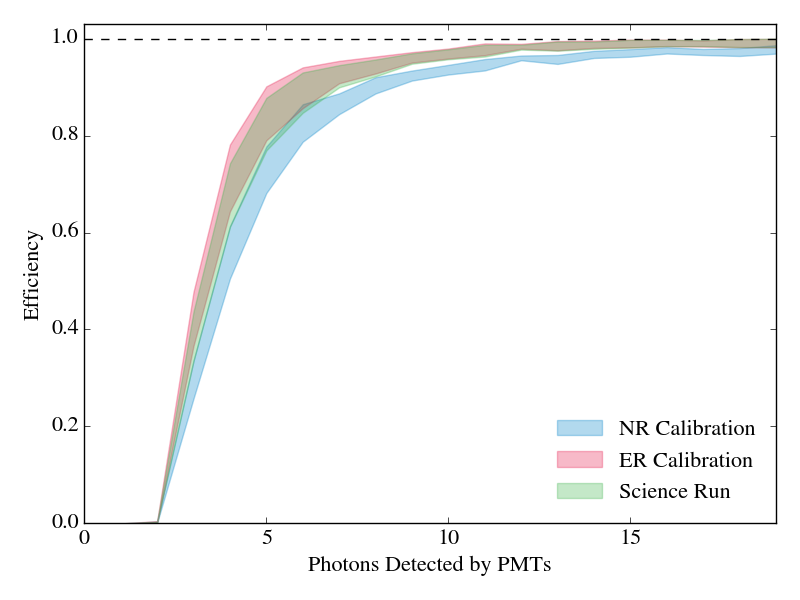
\includegraphics[width=0.85\textwidth]{xe1t_pax_acceptance}
	\caption{The estimated processor efficiency for identifying S1 signals in XENON1T.  These efficiencies were found via simulation and the shaded region represents the equally probable values for the efficiency at a given photon level.}
	\label{fig:xe1t_pax_acceptance}
\end{figure}


The bias and the smearing represent the changing of the signal area due to processor and PMT effects.  Like the processor efficiency, these effects are only expected to be relevant for very small signals and they are very hard to directly measure.  The results from simulation using XENON1T's waveform simulation are shown in \figref{fig:xe1t_pax_sb}.  Both bias and smearing are shown as $\frac{\textrm{Processed} - \textrm{Truth}}{\textrm{Truth}}$.  The shaded regions again can be thought of as a uniform distribution from which the bias and smearing can take any value for a given number of photons detected.  Note that the bias and smearing for the first science run and the electronic recoil calibration were similar enough that they are not treated separately.

\begin{figure}[t]
	\centering
	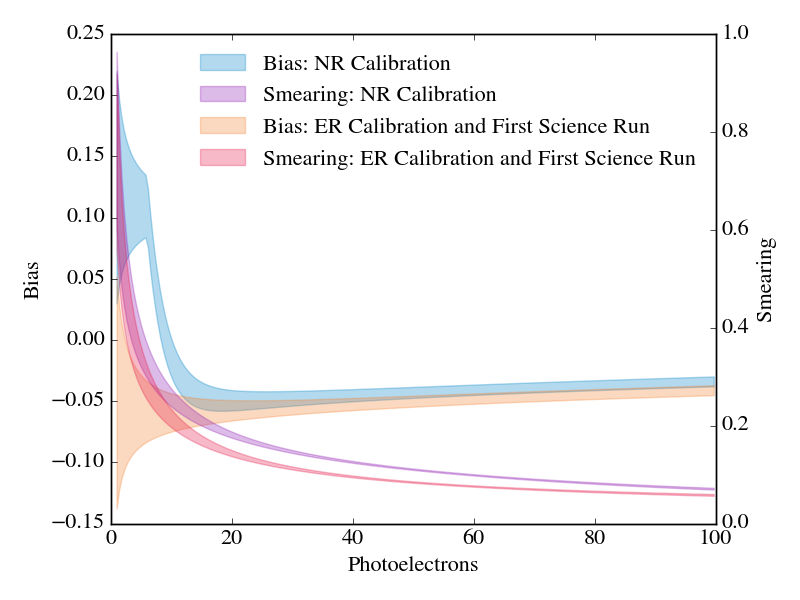
\includegraphics[width=0.85\textwidth]{xe1t_pax_s1_bias}
	\caption{The estimated bias and smearing of S1 signals due to the processing of the waveform for scintillation signals.}
	\label{fig:xe1t_pax_sb}
\end{figure}

With the processor efficiency accounted for given the number of photons that create at least one photoelectron, we may now account for the double photoelectron effect.  

\begin{equation}
        N_{\textrm{PE}} \sim N_{\textrm{i}} + B(N=N_{\textrm{i}}, p=p_{\textrm{DPE}})
\end{equation}


While the processor efficiency is used to ultimately set a weight on a given Monte Carlo event for the histogram that will be compared to data, the effect of the bias and smearing were approximated using \eqnref{eqn:xe1t_s1_bias} and \eqnref{eqn:xe1t_s1_smearing}, respectively.  

\begin{equation}
        \label{eqn:xe1t_s1_bias}
        \textrm{S1'} = \frac{N_{\textrm{PE}}}{1 + b}
\end{equation}


\begin{equation}
        \label{eqn:xe1t_s1_smearing}
        \textrm{S1} \sim N(\mu = \textrm{S1'}, \sigma^2 = (\textrm{S1'} \cdot s)^2)
\end{equation}


With the reconstructed and uncorrected S1 determined, we can find the probability that this good event would have been removed by a cut via the cut acceptance shown in \figref{fig:xe1t_cut_acceptances}.  We will multiply this probability with the probability that the signal is found by the processor to ultimately set the weight of the event (after S2 losses are considered since we require both an S1 and S2 in an acceptable waveform).


With processor, PMT, and cut effects accounted for, we now have the uncorrected S1 for a given interaction along with the probability that it would actually be discovered in a waveform.  Since the data that the Monte Carlo result will be compared to is corrected, we will also correct the simulated S1 signals.  This correction is shown in \eqnref{eqn:xe1t_s1_recorrect}, where 

\begin{equation}
        \label{eqn:xe1t_s1_recorrect}
        \textrm{cS1} = \frac{\textrm{S1}}{c_{\textrm{LCE}}(r, z)}
\end{equation}




\paragraph{Detection of Electrons}
\label{sec:xe1t_mc_electrons}


The first detector process that needs to be considered for the electrons extracted from the interaction site is their drifting to the liquid-gas interface.  During this drifting, their is a measurable probability that an extracted electron will attach to an electronegative impurity.  This probability, shown in \eqnref{eqn:xe1t_electron_lifetime} (repeated below), is dependent on the depth, the drift velocity through the xenon at the given field, and the electron lifetime.   

\begin{equation}
        \tag{\ref{eqn:xe1t_electron_lifetime}}
        p_{\textrm{EL}}(z) = \frac{1}{\tau_{e^-}} e^{-\frac{z}{v_d \tau_{e}}}
\end{equation} 


The electron lifetime is a function of the outgassing rate of the various detector components and the rate at which the xenon is being cleaned and is thus constantly changing as a function of time.  This change in time is clearly shown in \figref{fig:xe1t_electron_lifetime_sr0}.

We approximate the number of electrons that reach the liquid-gas interface by assuming that each of the extracted electrons is independent and thus the number of electrons reaching the interface is described by a binomial distribution as shown in \eqnref{eqn:xe1t_binomial_el}.


\begin{equation}
        \label{eqn:xe1t_binomial_el}
        N_{\textrm{L-G Interface}} \sim B \left( N=N_e, p=p_{\textrm{EL}}(z) \right)
\end{equation}


In \eqnref{eqn:xe1t_binomial_el}, $N_{\textrm{L-G Interface}}$ is the number of electrons that reach to the liquid-gas interface, $N_e$ is the number of electrons extracted from the interaction site, and $p_{\textrm{EL}}(z)$ is the probability of an individual electron reaching the liquid-gas interface as given by \eqnref{eqn:xe1t_electron_lifetime}.  Note that the variation in the number of electrons reaching the liquid-gas interface increases as the electron lifetime decreases.

As discussed in \secref{sec:xe1t_anticorrelation}, not all electrons that reach the liquid-gas interface will be extracted into the gaseous xenon in a meaningful timeframe.  Therefore, we approximate that the number of electrons extracted into the gas is described by another binomial process with the number of trials equal to $N_{\textrm{L-G Interface}}$ and probability of extraction equal to the extraction efficiency, as shown in \eqnref{eqn:xe1t_binomial_ee}.

\begin{equation}
        \label{eqn:xe1t_binomial_ee}
        N_{\textrm{extracted}} \sim B \left( N= N_{\textrm{L-G Interface}}, p=p_{\textrm{extracted}} \right)
\end{equation}


With the number of electrons extracted from the gas, we can next account for excitation caused by these electrons in the gaseous xenon as well as the smearing due to the PMTs.  We approximate the number of photoelectrons detected in this secondary amplification as Gaussian process as shown in \eqnref{eqn:xe1t_gas_gain} where $G$ is the mean number of photoelectrons detected for a single extracted electron, $\sigma_G$ is the width of the photoelectron distribution for a single extracted electron, $c_{G}(x, y)$ is the position correction of the gas gain as shown in \figref{fig:xe1t_s2_correction_map_xy}, and $N_{\textrm{PE}}$ is the number of photoelectrons digitized after smearing from the PMTs.

\begin{equation}
        \label{eqn:xe1t_gas_gain}
        N_{\textrm{PE}} \sim N(\mu=G \cdot c_{G}(x, y), \sigma^2=\sigma_G \cdot c_{G}(x, y))
\end{equation}


While no efficiency is applied to the total S2 signal from the processor or the trigger, we do remove uncorrected S2 signals under the defined threshold of 200 photoelectrons.  This cut is made to ensure nearly 100\% efficiency of the trigger.


%The bias and the smearing represent the changing of the signal area due to processor and PMT effects.  Like the processor efficiency, these effects are only expected to be relevant for very small signals and they are very hard to directly measure.  The results from simulation using XENON1T's waveform simulation are shown in \figref{fig:xe1t_pax_sb}.  Both bias and smearing are shown as $\frac{\textrm{Processed} - \textrm{Truth}}{\textrm{Truth}}$.  The shaded regions again can be thought of as a uniform distribution from which the bias and smearing can take any value for a given number of photons detected.  Note that the bias and smearing for the first science run and the electronic recoil calibration were similar enough that they are not treated separately.

Like the S1 signal, the S2 signal will also experience some bias and smearing during reconstruction of the event by the processor, albeit to a smaller degree.  Again both bias and smearing are shown as $\frac{\textrm{Processed} - \textrm{Truth}}{\textrm{Truth}}$ in \figref{fig:xe1t_s2_sb} and the shaded regions again can be thought of as a uniform distribution from which the bias and smearing can take any value for a given number of photons detected.  

\begin{figure}[t]
	\centering
	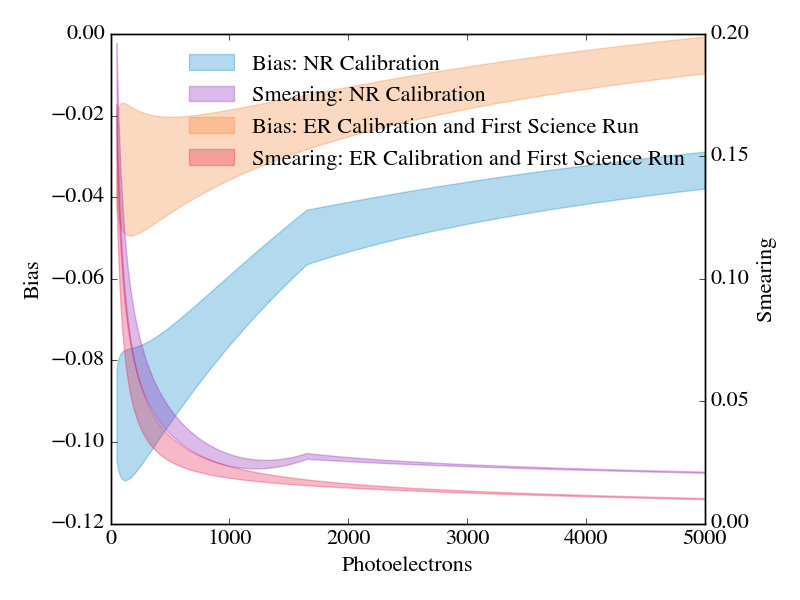
\includegraphics[width=0.85\textwidth]{xe1t_pax_s2_bias}
	\caption{The estimated bias and smearing of S2 signals due to the processing of the waveform for scintillation signals.}
	\label{fig:xe1t_s2_sb}
\end{figure}


We apply the effects of the processor bias and efficiency in the same way as the S1 signal in the Monte Carlo, as shown in \eqnref{eqn:xe1t_s2_bias} and \eqnref{eqn:xe1t_s2_smearing}.  

\begin{equation}
        \label{eqn:xe1t_s2_bias}
        \textrm{S2'} = \frac{N_{\textrm{PE}}}{1 + b}
\end{equation}


\begin{equation}
        \label{eqn:xe1t_s2_smearing}
        \textrm{S2} \sim N(\mu = \textrm{S2'}, \sigma^2 = (\textrm{S2'} \cdot s)^2)
\end{equation}

With the reconstructed and uncorrected S2 determined, we can find the probability that this good event would have been removed by a cut via the cut acceptance shown in Fig. 3.25. We will multiply this probability with the associated S1 signal's efficiencies to find the overall probability that the event would be seen in our dataset, as shown in \eqnref{eqn:xe1t_event_weight}.  This probability is used as the weight of the Monte Carlo event when filling the two-dimensional histogram for comparison to data.

\begin{equation}
        \label{eqn:xe1t_event_weight}
        p_{\textrm{event}} = p_{\textrm{Processor-S1}} \cdot p_{\textrm{Cuts-S1}} \cdot p_{\textrm{Cuts-S2}}
\end{equation}

Finally, for comparison to data, we must finally correct our S2 signal according to the electron lifetime and position correction of the gas gain, as shown in \figref{eqn:s2_correction}


\begin{equation}
        \label{eqn:s2_correction}
        \textrm{cS2} = \frac{\textrm{S2}}{p_{\textrm{EL}}(z) c_G(x, y)} 
\end{equation}


\subsubsection{Comparing Data and Monte Carlo}
\label{sec:xe1t_mc_electrons}

With the full Monte Carlo simulation in place, examining the expected distribution electronic or nuclear recoil distribution given input energy and position spectra is straightforward.  At the end of the day, though, what we would like to do is find the probability distribution for the observables model given the data that was measured in XENON1T.  This means that the ability to simulate the electronic or nuclear recoil spectra is not enough: we must be able to quantitatively compare the Monte Carlo results for a given set of parameters and the data.

Fortunately, this comparison is quite straightforward.  In these analyses, the simple binned likelihood function was used to compare data and the fast Monte Carlo.  We will cover the details, assumptions, and subtleties of this choice in the next chapter.  The likelihood function is shown in \eqnref{eqn:xe1t_binned_likelihood}, where $\mathcal{L}_i$ is the likelihood of a given bin, $\hat{b}_i$ is the expected number of events in a given bin, and $b_i$ is the measured number of events in a given bin.

\begin{equation}
        \label{eqn:xe1t_binned_likelihood}
        \begin{gathered}
                \mathcal{L}_i = \frac{\hat{b}_i^{b_i} e^{-\hat{b}_i}}{b_i!} \implies \mathcal{L} = \prod_i \mathcal{L}_i \\ 
                ln(\mathcal{L}) = \sum_i ln(\mathcal{L}_i) = \sum_i ( b_i ln(\hat{b}_i) - \hat{b}_i - ln(b_i!) )
        \end{gathered}
\end{equation}


As with any parameter estimation, the more parameters that you can independently constrain prior to the fit, the more you can say about parameters of interest.  In both the electronic and nuclear recoil calibrations almost all of the detector parameters were constrained and in the nuclear recoil calibration the light and charge production model was also constrained.  These constraints are also referred to as \textit{prior distributions} in Bayesian analyses (and colloquially referred to as \textit{penalty terms} in frequentist analyses).  The prior distributions in these analyses all take the form of normal distributions (asymmetric if asymmetric uncertainties are given) and ranged uniform distributions.  Unknown parameters still require a prior --- for example, many parameters, while unmeasured, we know cannot be negative.  These unknown parameters are given uniform priors that are bounded by zero if necessary.


In Bayesian analyses, our ultimate goal is to estimate the posterior distribution of the parameters one is trying to measure given the data that was collected.  The posterior probability is directly proportional to the likelihood multiplied by the prior distribution and given by Bayes' formula, shown in \eqnref{eqn:xe1t_bayes_formula} \cite{bayes1763essay}.

\begin{equation}
        \label{eqn:xe1t_bayes_formula}
        p(\vec{\theta}|\vec{x}) = \frac{p(\vec{x}|\vec{\theta}) p(\vec{\theta})}{p(\vec{x})} = \frac{\mathcal{L}(\vec{\theta}) p(\vec{\theta})}{p(\vec{x})}
\end{equation}


In the above equation, $p(\vec{x}|\vec{\theta})$ is probability of the data given the parameters, otherwise known as the likelihood, and $p(\vec{\theta})$ is the prior probabilities of the parameters.  The denominator in Bayes' formula is not as simple.  $p(\vec{x})$ is the probability of the data given the model, which is given by \eqnref{eqn:xe1t_px}.


\begin{equation}
        \label{eqn:xe1t_px}
        p(\vec{x}) = \int_{\Theta} p(\vec{x}|\vec{\theta}) d\vec{\theta}
\end{equation}


While it may not appear daunting, $p(\vec{x})$ is simply incalculable for almost all models and the models used in these analyses are no exception.  We will discuss in \secref{sec:xe1t_mcmc} a clever way around this problem using a Markov Chain Monte Carlo (MCMC).

% maybe tables with model parameters here or in results section



\subsubsection{Estimating the Posterior Probability Distribution Using a Markov Chain Monte Carlo}
\label{sec:xe1t_mcmc}

% brief discussion of MCMC and intuitive description of how it works

Markov Chain Monte Carlos (MCMCs) have arguably become one of the most popular statistical tools in the last decade.  In essence, they operate by randomly sampling from the posterior distribution.  Given enough samples from your MCMC, you can approximate the complete shape of the posterior.  With computer processors drastically increasing in speed, the ultimate cost of more function calls versus a traditional parameter estimation tool is dominated by the gain in getting a full understanding of the posterior probability distribution.

While a proof that an MCMC can randomly sample from the posterior distribution is far beyond the scope of this work, it is worthwhile to briefly discuss an intuitive description of how an MCMC works.  In the previous section, we mentioned Bayes' formula and how we might directly calculate the posterior probability distribution.  However, we ran into an issue with the denominator, which for all practical purposes is incalculable.  An MCMC uses a simple alternative to get around this issue:  

\begin{enumerate}
        \item Start at a given position in parameter space and calculate the likelihood function multiplied by the prior probability of that position, $f_0 = \mathcal{L}(\vec{\theta_0}) p(\vec{\theta_0})$.  
        \item Examine a new, randomly chosen position in parameter space and calculate $f_1 = \mathcal{L}(\vec{\theta_1}) p(\vec{\theta_1})$.
        \item Calculate the ratio $\mathcal{A} = \frac{f_1}{f_0}$.  If $\mathcal{A} \geq 1$, we accept the proposed step and ``move'' to this position in parameter space.  If $\mathcal{A} < 1$, we accept the proposed step with a probability $\mathcal{A}$ and otherwise stay in place in parameter space.  
        \item Record the current position in parameter space, $\theta_0$ or $\theta_1$, and repeat the above procedure.
\end{enumerate}

This procedure, if allowed to continue indefinitely, will produce random samples from the posterior distribution.  The reason for this can be seen in our calculation of $\mathcal{A}$.  If we can manipulate our definition of to put it in a more familiar form.

\begin{equation}
        \mathcal{A} = \frac{f_1}{f_0} = \frac{\mathcal{L}(\vec{\theta_1}) p(\vec{\theta_1})}{\mathcal{L}(\vec{\theta_0}) p(\vec{\theta_0})} \cdot \frac{p(\vec{x})}{p(\vec{x})} = \frac{\frac{\mathcal{L}(\vec{\theta}_1) p(\vec{\theta}_1)}{p(\vec{x})}}{\frac{\mathcal{L}(\vec{\theta}_0) p(\vec{\theta}_0)}{p(\vec{x})}} = \frac{p(\vec{x}|\vec{\theta}_1)}{p(\vec{x}|\vec{\theta}_0)}
\end{equation}

It turns out that our acceptance ratio is simply the ratio of the posterior probability distribution at our two points in parameter space.  We don't simply climb to higher positions in the posterior because we allow for non-zero probability jumps to lower positions in the posterior.

In these analyses, and all others discussed in this work that use a MCMC, the affine-invariant implementation of the MCMC algorithm was used.  This implementation is discussed in detail in \citeref{foreman2013emcee} but in summary it uses multiple MCMC chains to probe the parameter space more efficiently.  These chains use each other to decide their next step in a more intelligent way versus the very basic Metropolis-Hastings single chain algorithm \cite{chib1995understanding}.  Ultimately, all of the MCMC chains will randomly sample the posterior and can be combined such that the efficiency gains from ``intelligent'' step choices are not lost to high levels of redundancy.

In theory, an MCMC is not guaranteed to converge until infinite steps are taken.  In practice, however, MCMCs typically converge in reasonable amounts of steps.  Several tests can be performed to test the convergence of the chain into the posterior, a few of which are discussed in detail in \citeref{brooks1998general}.  In this work, we will use the Gelman-Rubin statistic to check the convergence of our MCMC \cite{gelman1992inference}.  The Gelman-Rubin statistic in essence examines the average variance of individual chains to the variance between chains.  For chains that begin separated from each other in parameter space, this mixing is a good proxy for convergence of the chains.

% mention the indefinite portion in first sentence of last paragraph

% brief discussion of MCMC used for these analyses emcee


\subsection{ER and NR Calibration Results}
\label{sec:xe1t_er_nr_results}

With the procedure, models, and Monte Carlo details outline, we can move to the results of the two calibrations.  Ideally, these calibrations would be performed simultaneously due to the overlap between the two from the detector model.  However, in the first science run they were performed separately as a proof of principle.


\subsubsection{Results of the Electronic Recoil Calibration}

The electronic recoil calibration was performed with the microphysics model described in \secref{sec:xe1t_mc_observables_production_er} and the detector physics model described in \secref{sec:xe1t_mc_detector}.  The list of model parameters included in the fit for the light and charge production model for electronic recoils is shown in \tabref{tab:xe1t_er_model_pars} while the parameters of the detector model are shown in \tabref{tab:xe1t_detector_pars}.  Note that the detector physics parameters will be shared with the nuclear recoil calibration.

In total, eight free parameters were included in the observables production model for electronic recoils: five from the fourth-order polynomial used to describe the light yield relative to a reference curve, one from the energy threshold for recombination (below which recombination no longer is considered), and two for the parameterization of the recombination fluctuation ($\Delta r = A \cdot (1 - e^{\sfrac{E}{\tau_r}})$).  The reference curve use for the light yield is given by \citeref{szydagis2013enhancement} with a mean field of 120 V/cm.  With both the light yield, mean energy per quanta, and exciton-to-ion ratio, the mean value for recombination can be reconstructed.  



\begin{table}[b]
\centering
\def\arraystretch{1.3}
\resizebox{\textwidth}{!}{
\begin{tabular}{|c|c|c|c|}

\hline
Parameter & Value & Prior Distribution & Note  \\
\hline
$w$ & $13.7 \pm 0.2$ eV & Normal & - \\ \hline
$F$ & 0.059 & Fixed & - \\ \hline
$\sfrac{N_{\textrm{ex}}}{N_{\textrm{ion}}}$ & 0.06--0.20 & Uniform & Taken from \citeref{szydagis2011nest}. \\ \hline
Accidental Coincidence Background & $1.22 \cdot 10^{-6} \pm 7.32 \cdot 10^{-8}$ Hz & Normal & - \\ \hline
Photon Yield (5) & - & \textbf{Free} & - \\ \hline
Recombination Fluctuation (2) & - & \textbf{Free} & - \\ \hline
Energy Threshold (1) & - & \textbf{Free} & - \\ \hline
\end{tabular}}
\caption{The parameters of the light and charge model for electronic recoils in liquid xenon. Note that the parameters described as free in the fit are unrestricted (barring physical limitations).}
\label{tab:xe1t_er_model_pars}
\end{table}


\begin{table}[b]
\centering
\def\arraystretch{1.3}
\resizebox{\textwidth}{!}{
\begin{tabular}{|c|c|c|c|}

\hline
Parameter & Value & Prior Distribution & Note  \\
\hline
$g_1$ & $0.1442 \pm 0.0068$ & Normal & - \\ \hline
$p_{\textrm{DPE}}$ & 0.18--0.24 & Uniform & Taken from \citeref{faham2015measurements}. \\ \hline
$p_{\textrm{extracted}}$ & $0.961 \pm 0.046$ & Normal & - \\ \hline
$G_{\textrm{bottom}}$ & $11.69 \pm 0.26$ & Normal & - \\ \hline
$\sigma_{G_{\textrm{bottom}}}$ & $2.80$ & Fixed & - \\ \hline
Processor Efficiency & - & Uniform & Uniform inside bounds of \figref{fig:xe1t_pax_acceptance}. \\ \hline
Processor S1 Bias & - & Uniform & Uniform inside bounds of \figref{fig:xe1t_pax_sb}. \\ \hline
Processor S1 Smearing & - & Uniform & Uniform inside bounds of \figref{fig:xe1t_pax_sb}. \\ \hline
Processor S2 Bias & - & Uniform & Uniform inside bounds of \figref{fig:xe1t_s2_sb}. \\ \hline
Processor S2 Smearing & - & Uniform & Uniform inside bounds of \figref{fig:xe1t_s2_sb}. \\ \hline
S1 Correction Map & - & Fixed & Shown in \figref{fig:xe1t_s1_correction_map}. \\ \hline
S2 Correction Map & - & Fixed & Shown in \figref{fig:xe1t_s2_correction_map_xy}. \\ \hline
Electron Lifetime & - & Fixed & Randomly drawn from measured electron lifetimes. \\ \hline
S2 Fraction - Bottom & 0.38 & Fixed & - \\ \hline
Total S2 Threshold & 200 & Fixed & - \\ \hline
S1 Cut Acceptance & - & Normal & Mean and width shown in \figref{fig:xe1t_cut_acceptances}. \\ \hline
S2 Cut Acceptance & - & Normal & Mean and width shown in \figref{fig:xe1t_cut_acceptances}. \\ \hline
\end{tabular}}
\caption{The detector model parameters and their associated priors.  Note that all of these parameters is tightly constrained by independent calibrations.}
\label{tab:xe1t_detector_pars}
\end{table}


One parameter that has not been mentioned prior to now is the accidental coincidence background rate.  In XENON1T, it has been found that there is a relatively high rate of lone-S1 signals and lone-S2 signals.  While the causes of each vary from interactions in the liquid xenon below the cathode to interactions in the gaseous xenon, if an S1 and S2 are coincident within a given time window they can together be mistaken for a real event.  This background is source dependent and will therefore be different for dark matter data and the electronic recoil calibrations (the accidental coincidence background was found to be negligible for the nuclear recoil calibration).  The probability distribution for the accidental coincidence background is shown in \figref{fig:xe1t_ac_bkg}.

\begin{figure}[t]
	\centering
	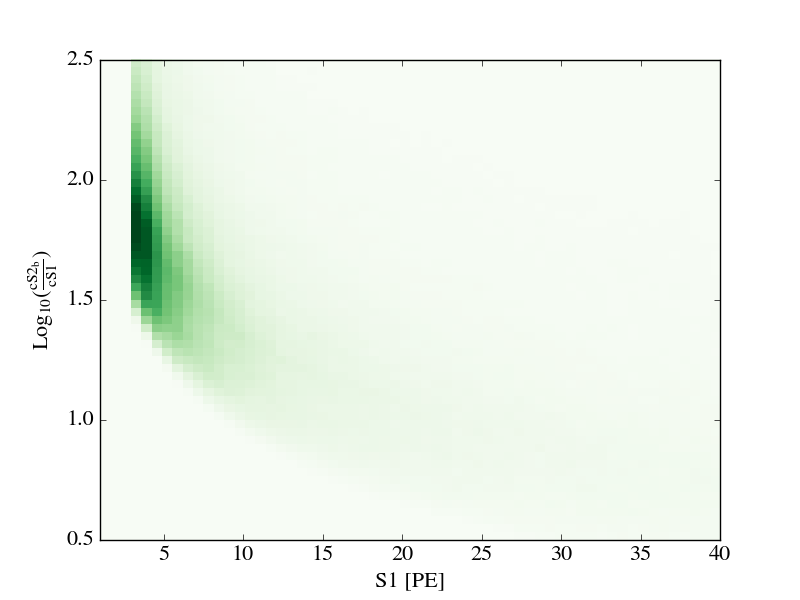
\includegraphics[width=0.8\textwidth]{xe1t_ac_bkg}
	\caption{The PDF of accidental coincidence background events in $\textrm{log} \left( \frac{\textrm{cS2}_{\textrm{b}}}{\textrm{cS1}} \right)$ space for the first dark matter run.}
	\label{fig:xe1t_ac_bkg}
\end{figure}



With the models and parameter estimation framework in place, the electronic recoil calibration can be performed.  The best-fit PDF, which can be predicted with the posterior distribution of the parameters, is shown in \figref{fig:xe1t_er_pdf_overlaid_data}.  Additionally, a comparison of the band shape, specifically the band median and width, is shown in \figref{fig:xe1t_er_band_width_median}.  One can see from both of these comparisons that the \ce{^{220}Rn} agrees extremely well with the model used.


\begin{figure}[p]
	\centering
	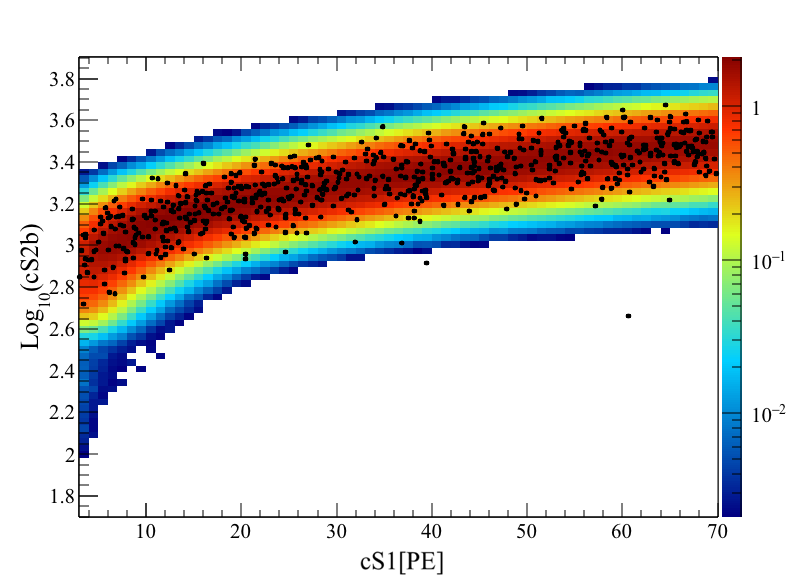
\includegraphics[width=0.9\textwidth]{xe1t_er_pdf_overlaid_data}
	\caption{The best-fit PDF for electronic recoils during the \ce{^{220}Rn} electronic recoil calibration.  Outside of the few two outliers, the agreement between the model and data is extremely good.}
	\label{fig:xe1t_er_pdf_overlaid_data}
	
	\centering
	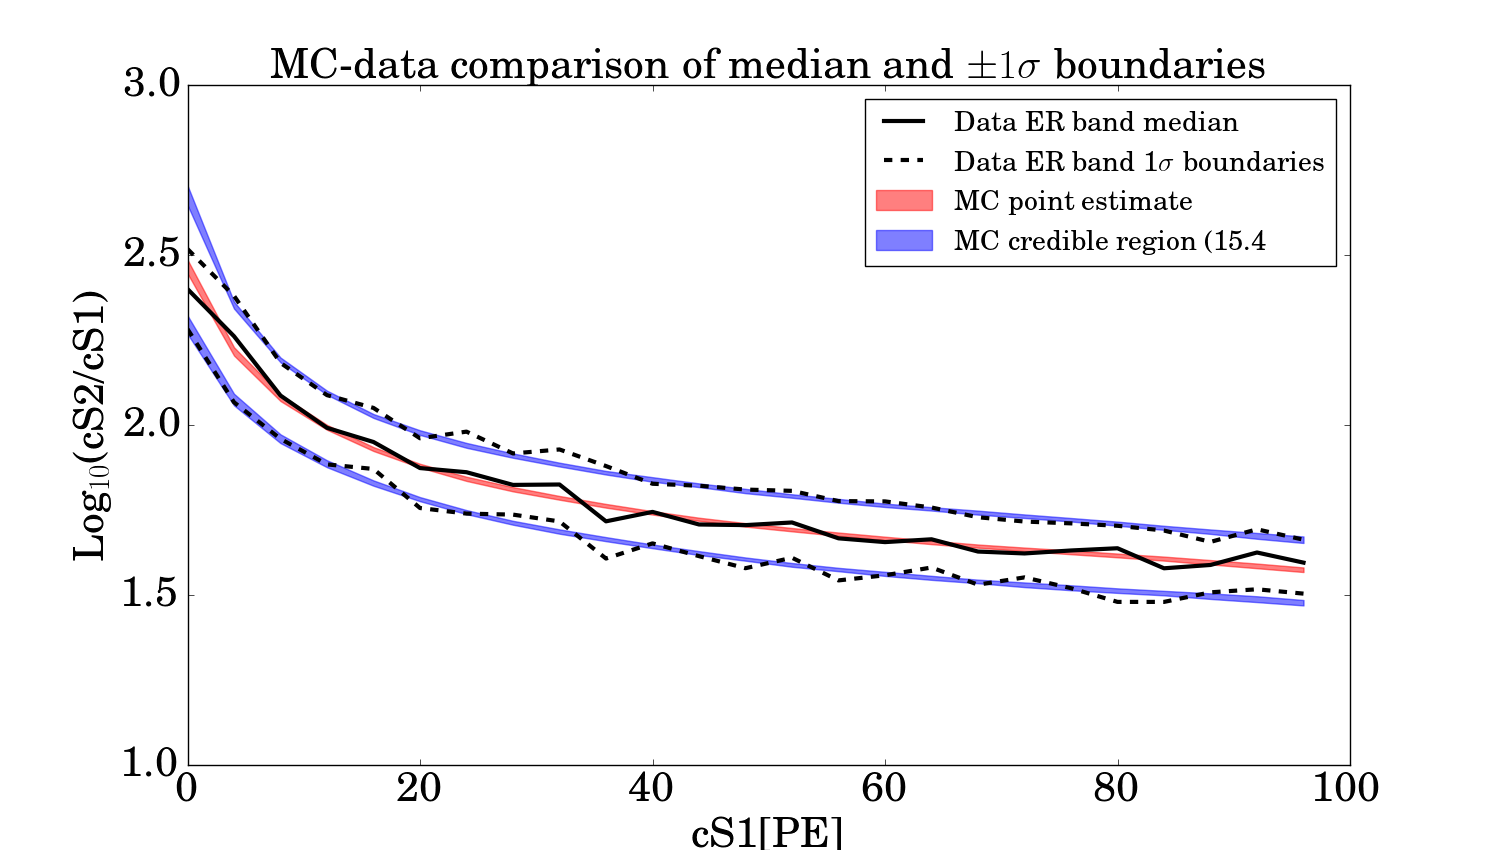
\includegraphics[width=0.9\textwidth]{xe1t_er_band_width_median}
	\caption{Comparison of the band median and width during the electronic recoil calibration.  One can see that the fit provides excellent agreement in the region of interest.}
	\label{fig:xe1t_er_band_width_median}
\end{figure}
	
	
One can also see the comparison of the model to data in S1 and S2 signal space only.  Again, there are no significant deviations or flaws in the model that are evident.
	
	
\begin{figure}[t]
	\centering
	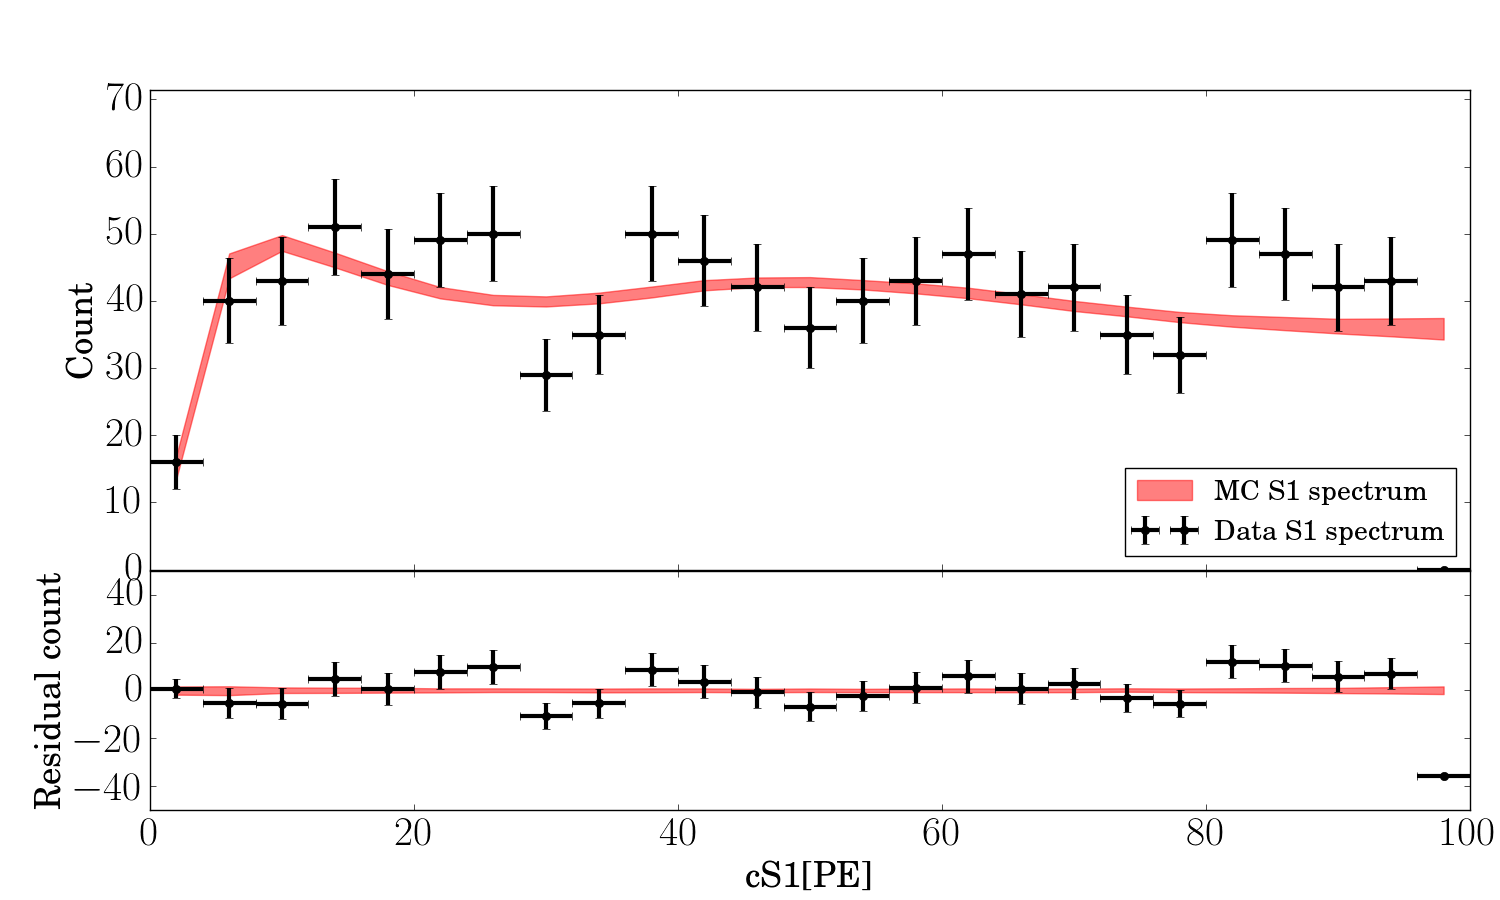
\includegraphics[width=0.99\textwidth]{xe1t_er_band_s1}
	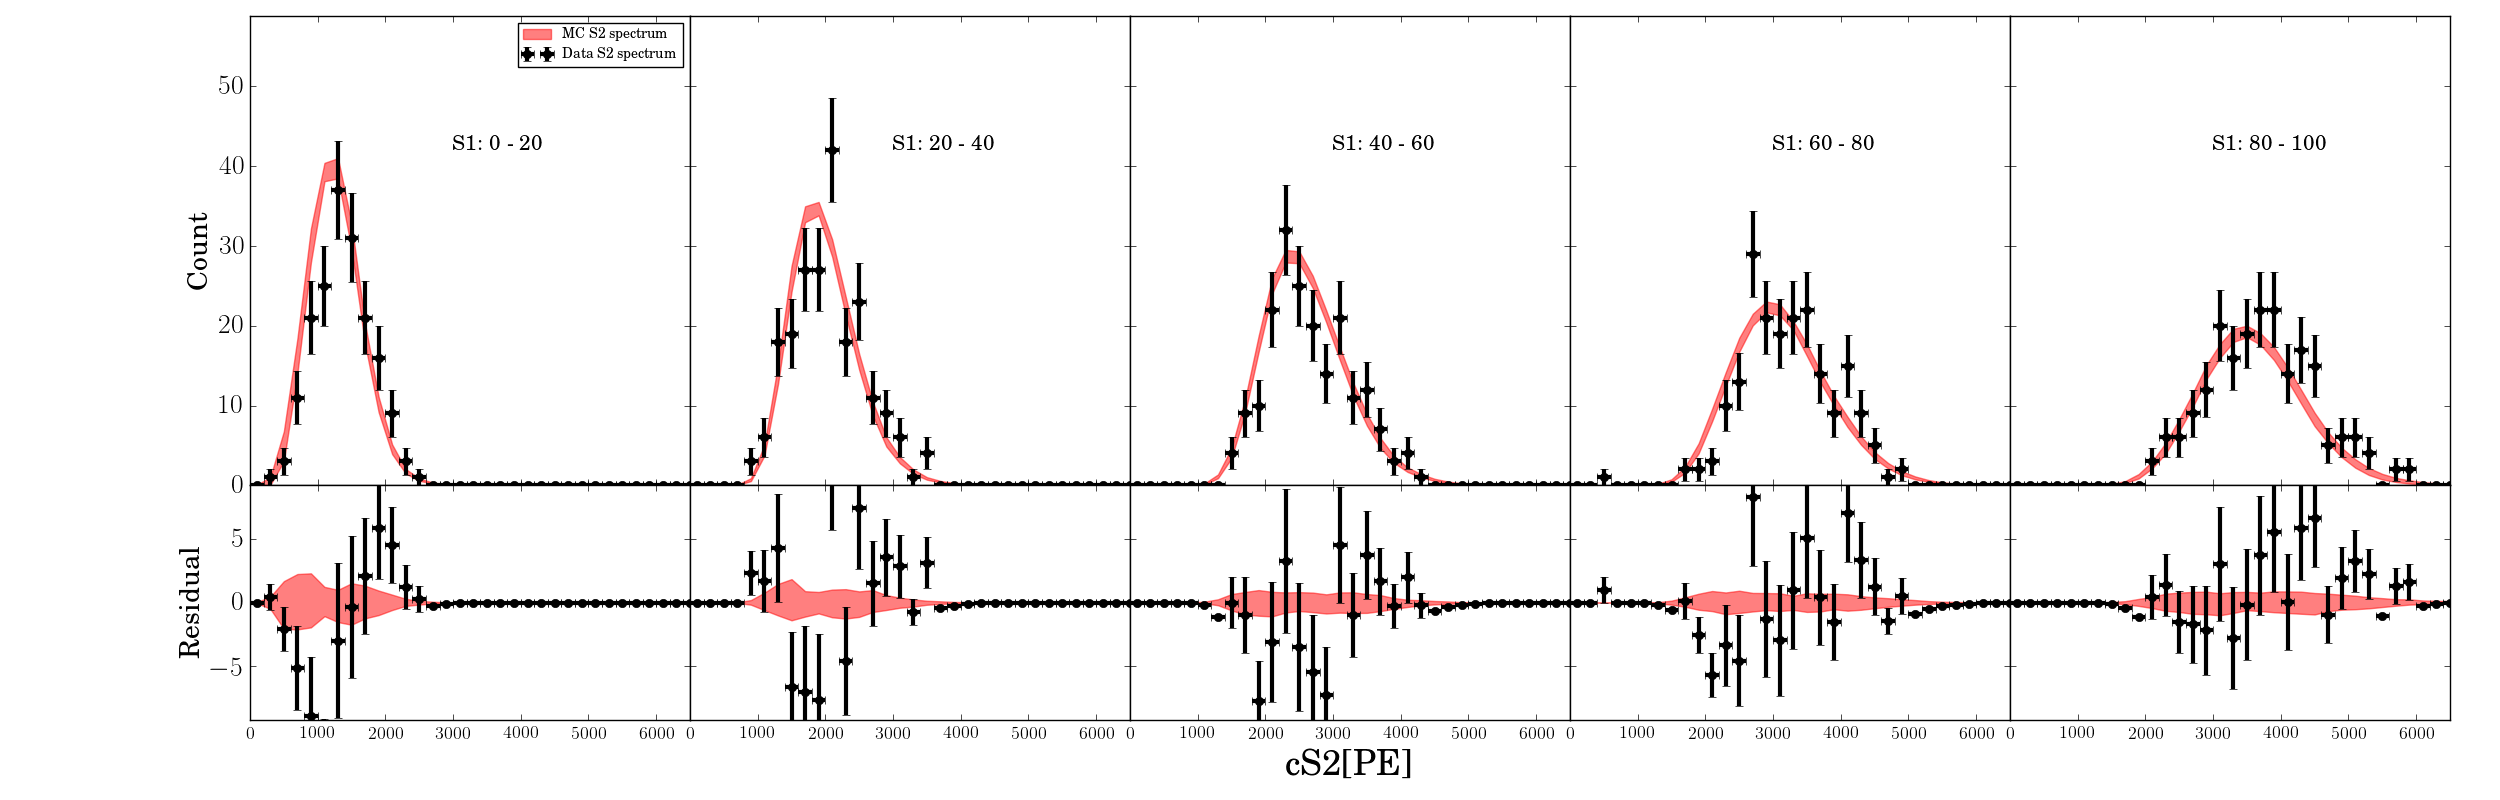
\includegraphics[width=0.99\textwidth]{xe1t_er_band_s2}
	\caption{Comparison of the band median and width during the electronic recoil calibration.  One can see that the fit provides excellent agreement in the region of interest.}
	\label{fig:xe1t_er_band_width_median}
\end{figure}





\subsubsection{Results of the Nuclear Recoil Calibration}

The nuclear recoil calibration was performed with the microphysics model described in \secref{sec:xe1t_mc_observables_production_nr} and the detector physics model described in \secref{sec:xe1t_mc_detector}.  Since the detector model parameters are the same as for the electronic recoil calibration, the list shown in \tabref{tab:xe1t_detector_pars} also applies for the nuclear recoil calibration.  The observables production parameters will be different for the nuclear recoil calibration and the parameters are listed in \tabref{}.


\begin{table}[b]
\centering
\def\arraystretch{1.3}
\resizebox{\textwidth}{!}{
\begin{tabular}{|c|c|c|c|}

\hline
Parameter & Value & Prior Distribution & Note  \\
\hline
$w$ & $13.7 \pm 0.2$ eV & Normal & - \\ \hline
$\alpha$ & $1.240^{+0.079}_{-0.073}$ & Normal & Taken from \citeref{lenardo2015global} \\ \hline
$\zeta$ & $0.0472^{+0.0088}_{-0.0073}$ & Normal & Taken from \citeref{lenardo2015global} \\ \hline
$\beta$ & $239^{+28}_{-8.8}$ & Normal & Taken from \citeref{lenardo2015global} \\ \hline
$\gamma$ & $0.01385^{+0.00058}_{-0.00073}$ & Normal & Taken from \citeref{lenardo2015global} \\ \hline
$\delta$ & $0.0620^{+0.0056}_{-0.0064}$ & Normal & Taken from \citeref{lenardo2015global} \\ \hline
$k$ & $0.1394^{+0.0032}_{-0.0026}$ & Normal & Taken from \citeref{lenardo2015global} \\ \hline
$\eta$ & $3.3^{+5.3}_{-0.7}$ & Normal & Taken from \citeref{lenardo2015global} \\ \hline
$\lambda$ & $1.14^{+0.45}_{-0.09}$ & Normal & Taken from \citeref{lenardo2015global} \\ \hline
Probability of ER Event & - & \textbf{Free} & - \\ \hline
\end{tabular}}
\caption{The parameters of the light and charge model for electronic recoils in liquid xenon. Note that the parameters described as free in the fit are unrestricted (barring physical limitations).}
\label{tab:xe1t_er_model_pars}
\end{table}

Note that the probability of the electronic recoil event is left free.  This parameter is a proxy for the electronic recoil background rate during the AmBe calibration.  The reason this must be included is simply because the \ce{^{222}Rn} background rate is not negligible during the nuclear recoil calibration and could potentially skew the fit to predict higher light and charge yields.  Therefore, we include this background by assuming that each event has a finite probability of being from the \ce{^{222}Rn}.  If the event is from our electronic recoil background, we use the best-fit model from the electronic recoil background and a uniform distribution in energy and position to simulate the event.

Note that the electronic recoil rate is left free.  Because the electronic recoil background during the nuclear recoil calibration is non-negligible, the nuclear recoil calibration must follow the electronic recoil calibration.  The best-fit electronic recoil model is used to model the background which is assumed to be flat (since it is from the decay of \ce{^{222}Rn}).  




\subsection{Propagating Results to the WIMP Search}
\label{sec:xe1t_propagating_results}





